% Options for packages loaded elsewhere
% Options for packages loaded elsewhere
\PassOptionsToPackage{unicode,linktoc=all,pdfwindowui,pdfpagemode=FullScreen,pdfpagelayout=TwoPageRight}{hyperref}
\PassOptionsToPackage{hyphens}{url}
\PassOptionsToPackage{dvipsnames,svgnames,x11names}{xcolor}
%
\documentclass[
  9pt,
  letterpaper,
  abstract,
  titlepage]{scrbook}
\usepackage{xcolor}
\usepackage[left=1in,marginparwidth=2.0666666666667in,textwidth=4.1333333333333in,marginparsep=0.3in]{geometry}
\usepackage{amsmath,amssymb}
\setcounter{secnumdepth}{3}
\usepackage{iftex}
\ifPDFTeX
  \usepackage[T1]{fontenc}
  \usepackage[utf8]{inputenc}
  \usepackage{textcomp} % provide euro and other symbols
\else % if luatex or xetex
  \usepackage{unicode-math} % this also loads fontspec
  \defaultfontfeatures{Scale=MatchLowercase}
  \defaultfontfeatures[\rmfamily]{Ligatures=TeX,Scale=1}
\fi
\usepackage{lmodern}
\ifPDFTeX\else
  % xetex/luatex font selection
\fi
% Use upquote if available, for straight quotes in verbatim environments
\IfFileExists{upquote.sty}{\usepackage{upquote}}{}
\IfFileExists{microtype.sty}{% use microtype if available
  \usepackage[]{microtype}
  \UseMicrotypeSet[protrusion]{basicmath} % disable protrusion for tt fonts
}{}
% Make \paragraph and \subparagraph free-standing
\makeatletter
\ifx\paragraph\undefined\else
  \let\oldparagraph\paragraph
  \renewcommand{\paragraph}{
    \@ifstar
      \xxxParagraphStar
      \xxxParagraphNoStar
  }
  \newcommand{\xxxParagraphStar}[1]{\oldparagraph*{#1}\mbox{}}
  \newcommand{\xxxParagraphNoStar}[1]{\oldparagraph{#1}\mbox{}}
\fi
\ifx\subparagraph\undefined\else
  \let\oldsubparagraph\subparagraph
  \renewcommand{\subparagraph}{
    \@ifstar
      \xxxSubParagraphStar
      \xxxSubParagraphNoStar
  }
  \newcommand{\xxxSubParagraphStar}[1]{\oldsubparagraph*{#1}\mbox{}}
  \newcommand{\xxxSubParagraphNoStar}[1]{\oldsubparagraph{#1}\mbox{}}
\fi
\makeatother

\usepackage{color}
\usepackage{fancyvrb}
\newcommand{\VerbBar}{|}
\newcommand{\VERB}{\Verb[commandchars=\\\{\}]}
\DefineVerbatimEnvironment{Highlighting}{Verbatim}{commandchars=\\\{\}}
% Add ',fontsize=\small' for more characters per line
\usepackage{framed}
\definecolor{shadecolor}{RGB}{242,244,248}
\newenvironment{Shaded}{\begin{snugshade}}{\end{snugshade}}
\newcommand{\AlertTok}[1]{\textcolor[rgb]{1.00,0.00,0.00}{\textbf{#1}}}
\newcommand{\AnnotationTok}[1]{\textcolor[rgb]{0.38,0.63,0.69}{\textbf{\textit{#1}}}}
\newcommand{\AttributeTok}[1]{\textcolor[rgb]{0.82,0.10,0.26}{#1}}
\newcommand{\BaseNTok}[1]{\textcolor[rgb]{0.25,0.63,0.44}{#1}}
\newcommand{\BuiltInTok}[1]{\textcolor[rgb]{0.88,0.40,0.10}{#1}}
\newcommand{\CharTok}[1]{\textcolor[rgb]{0.25,0.44,0.63}{#1}}
\newcommand{\CommentTok}[1]{\textcolor[rgb]{0.41,0.45,0.49}{\textit{#1}}}
\newcommand{\CommentVarTok}[1]{\textcolor[rgb]{0.38,0.63,0.69}{\textbf{\textit{#1}}}}
\newcommand{\ConstantTok}[1]{\textcolor[rgb]{0.53,0.00,0.00}{#1}}
\newcommand{\ControlFlowTok}[1]{\textcolor[rgb]{0.86,0.20,0.18}{\textbf{#1}}}
\newcommand{\DataTypeTok}[1]{\textcolor[rgb]{0.56,0.13,0.00}{#1}}
\newcommand{\DecValTok}[1]{\textcolor[rgb]{0.58,0.00,0.30}{#1}}
\newcommand{\DocumentationTok}[1]{\textcolor[rgb]{0.73,0.13,0.13}{\textit{#1}}}
\newcommand{\ErrorTok}[1]{\textcolor[rgb]{0.75,0.00,0.00}{\textbf{#1}}}
\newcommand{\ExtensionTok}[1]{\textcolor[rgb]{0.00,0.00,0.00}{#1}}
\newcommand{\FloatTok}[1]{\textcolor[rgb]{0.88,0.40,0.10}{#1}}
\newcommand{\FunctionTok}[1]{\textcolor[rgb]{0.42,0.37,0.78}{#1}}
\newcommand{\ImportTok}[1]{\textcolor[rgb]{0.00,0.45,0.70}{\textbf{#1}}}
\newcommand{\InformationTok}[1]{\textcolor[rgb]{0.38,0.63,0.69}{\textbf{\textit{#1}}}}
\newcommand{\KeywordTok}[1]{\textcolor[rgb]{0.73,0.49,0.84}{\textbf{#1}}}
\newcommand{\NormalTok}[1]{\textcolor[rgb]{0.00,0.00,0.00}{#1}}
\newcommand{\OperatorTok}[1]{\textcolor[rgb]{0.10,0.10,0.10}{#1}}
\newcommand{\OtherTok}[1]{\textcolor[rgb]{0.00,0.44,0.13}{#1}}
\newcommand{\PreprocessorTok}[1]{\textcolor[rgb]{0.74,0.48,0.00}{#1}}
\newcommand{\RegionMarkerTok}[1]{\textcolor[rgb]{0.00,0.00,0.00}{#1}}
\newcommand{\SpecialCharTok}[1]{\textcolor[rgb]{0.25,0.44,0.63}{#1}}
\newcommand{\SpecialStringTok}[1]{\textcolor[rgb]{0.73,0.40,0.53}{#1}}
\newcommand{\StringTok}[1]{\textcolor[rgb]{0.12,0.55,0.30}{#1}}
\newcommand{\VariableTok}[1]{\textcolor[rgb]{0.00,0.00,0.00}{#1}}
\newcommand{\VerbatimStringTok}[1]{\textcolor[rgb]{0.25,0.44,0.63}{#1}}
\newcommand{\WarningTok}[1]{\textcolor[rgb]{0.38,0.63,0.69}{\textbf{\textit{#1}}}}

\providecommand{\tightlist}{%
  \setlength{\itemsep}{0pt}\setlength{\parskip}{0pt}}\usepackage{longtable,booktabs,array}
\usepackage{calc} % for calculating minipage widths
% Correct order of tables after \paragraph or \subparagraph
\usepackage{etoolbox}
\makeatletter
\patchcmd\longtable{\par}{\if@noskipsec\mbox{}\fi\par}{}{}
\makeatother
% Allow footnotes in longtable head/foot
\IfFileExists{footnotehyper.sty}{\usepackage{footnotehyper}}{\usepackage{footnote}}
\makesavenoteenv{longtable}
\usepackage{graphicx}
\makeatletter
\newsavebox\pandoc@box
\newcommand*\pandocbounded[1]{% scales image to fit in text height/width
  \sbox\pandoc@box{#1}%
  \Gscale@div\@tempa{\textheight}{\dimexpr\ht\pandoc@box+\dp\pandoc@box\relax}%
  \Gscale@div\@tempb{\linewidth}{\wd\pandoc@box}%
  \ifdim\@tempb\p@<\@tempa\p@\let\@tempa\@tempb\fi% select the smaller of both
  \ifdim\@tempa\p@<\p@\scalebox{\@tempa}{\usebox\pandoc@box}%
  \else\usebox{\pandoc@box}%
  \fi%
}
% Set default figure placement to htbp
\def\fps@figure{htbp}
\makeatother
% definitions for citeproc citations
\NewDocumentCommand\citeproctext{}{}
\NewDocumentCommand\citeproc{mm}{%
  \begingroup\def\citeproctext{#2}\cite{#1}\endgroup}
\makeatletter
 % allow citations to break across lines
 \let\@cite@ofmt\@firstofone
 % avoid brackets around text for \cite:
 \def\@biblabel#1{}
 \def\@cite#1#2{{#1\if@tempswa , #2\fi}}
\makeatother
\newlength{\cslhangindent}
\setlength{\cslhangindent}{1.5em}
\newlength{\csllabelwidth}
\setlength{\csllabelwidth}{3em}
\newenvironment{CSLReferences}[2] % #1 hanging-indent, #2 entry-spacing
 {\begin{list}{}{%
  \setlength{\itemindent}{0pt}
  \setlength{\leftmargin}{0pt}
  \setlength{\parsep}{0pt}
  % turn on hanging indent if param 1 is 1
  \ifodd #1
   \setlength{\leftmargin}{\cslhangindent}
   \setlength{\itemindent}{-1\cslhangindent}
  \fi
  % set entry spacing
  \setlength{\itemsep}{#2\baselineskip}}}
 {\end{list}}
\usepackage{calc}
\newcommand{\CSLBlock}[1]{\hfill\break\parbox[t]{\linewidth}{\strut\ignorespaces#1\strut}}
\newcommand{\CSLLeftMargin}[1]{\parbox[t]{\csllabelwidth}{\strut#1\strut}}
\newcommand{\CSLRightInline}[1]{\parbox[t]{\linewidth - \csllabelwidth}{\strut#1\strut}}
\newcommand{\CSLIndent}[1]{\hspace{\cslhangindent}#1}

% =============================================================================
% LATEX HEADER CONFIGURATION FOR MLSYSBOOK PDF
% =============================================================================
% This file contains all LaTeX package imports, custom commands, and styling
% definitions for the PDF output of the Machine Learning Systems textbook.
%
% Key Features:
% - Harvard crimson branding throughout
% - Custom part/chapter/section styling
% - Professional table formatting with colored headers
% - Margin notes with custom styling
% - TikZ-based part dividers
% - Page numbering (Roman for frontmatter, Arabic for mainmatter)
%
% Note: This file is included via _quarto-pdf.yml and affects PDF output only.
% HTML/EPUB styling is handled separately via CSS files.
% =============================================================================

% =============================================================================
% PACKAGE IMPORTS
% =============================================================================

% Layout and positioning
% \usepackage[outercaption, ragged]{sidecap}  % Commented out to make figure captions inline instead of in margin
\usepackage{adjustbox}      % Adjusting box dimensions
\usepackage{afterpage}      % Execute commands after page break
\usepackage{morefloats}     % Increase number of floats
\usepackage{array}          % Enhanced table column formatting
\usepackage{atbegshi}       % Insert content at page beginning
%\usepackage{changepage}     % Change page dimensions mid-document
\usepackage{emptypage}      % Clear headers/footers on empty pages

% Language and text
\usepackage[english]{babel} % English language support
\usepackage{microtype}      % Improved typography and hyphenation

% Captions and floats
\usepackage{caption}
% Caption styling configuration
%\captionsetup[table]{belowskip=5pt}
\captionsetup{format=plain}
\DeclareCaptionLabelFormat{mylabel}{#1
#2:\hspace{1.0ex}}
\DeclareCaptionFont{ninept}{\fontsize{7pt}{8}\selectfont #1}

% Figure captions: Small font, bold label, ragged right
\captionsetup[figure]{labelfont={bf,ninept},labelsep=space,
belowskip=2pt,aboveskip=6pt,labelformat=mylabel,
justification=raggedright,singlelinecheck=false,font={ninept}}

% Table captions: Small font, bold label, ragged right
\captionsetup[table]{belowskip=6pt,labelfont={bf,ninept},labelsep=none,
labelformat=mylabel,justification=raggedright,singlelinecheck=false,font={ninept}}

% Typography fine-tuning
\emergencystretch=5pt       % Allow extra stretch to avoid overfull boxes

% Utility packages
\usepackage{etoolbox}       % For patching commands and environments

% Page layout and headers
\usepackage{fancyhdr}       % Custom headers and footers
\usepackage{geometry}       % Page dimensions and margins

% Graphics and figures
\usepackage{graphicx}       % Include graphics
\usepackage{float}          % Improved float placement
\usepackage[skins,breakable]{tcolorbox} % Coloured and framed text boxes
\tcbset{before upper=\setlength{\parskip}{3pt}}

% Tables
\usepackage{longtable}      % Multi-page tables

% Fonts and typography
\usepackage{fontspec}       % Font selection for LuaLaTeX
\usepackage{mathptmx}       % Times-like math fonts
\usepackage{newpxtext}      % Palatino-like font for body text

% Colors and visual elements
\usepackage[dvipsnames]{xcolor}  % Extended color support
\usepackage{tikz}           % Programmatic graphics
\usetikzlibrary{positioning}
\usetikzlibrary{calc}
\usepackage{tikzpagenodes}  % TikZ positioning relative to page

% Code listings
\usepackage{listings}       % Code highlighting

% Hyperlinks
\usepackage{hyperref}       % Clickable links in PDF

% Conditional logic
\usepackage{ifthen}         % If-then-else commands

% Math symbols
\usepackage{amsmath}        % AMS math extensions
\usepackage{amssymb}        % AMS math symbols
\usepackage{latexsym}       % Additional LaTeX symbols
\usepackage{pifont}         % Zapf Dingbats symbols
\providecommand{\blacklozenge}{\ding{117}}  % Black diamond symbol

% Lists
\usepackage{enumitem}       % Customizable lists

% Margin notes and sidenotes
\usepackage{marginfix}      % Fixes margin note overflow
\usepackage{marginnote}     % Margin notes
\usepackage{sidenotes}      % Academic-style sidenotes
\renewcommand\raggedrightmarginnote{\sloppy}
\renewcommand\raggedleftmarginnote{\sloppy}

% Typography improvements
\usepackage{ragged2e}       % Better ragged text
\usepackage[all]{nowidow}   % Prevent widows and orphans
\usepackage{needspace}      % Ensure minimum space on page

% Section formatting
\usepackage[explicit]{titlesec}  % Custom section titles
\usepackage{tocloft}        % Table of contents formatting

% QR codes and icons
\usepackage{fontawesome5}   % Font Awesome icons
\usepackage{qrcode}         % QR code generation
\qrset{link, height=15mm}

% =============================================================================
% FLOAT CONFIGURATION
% =============================================================================
% Allow more floats per page to handle figure-heavy chapters
\extrafloats{200}
\setcounter{topnumber}{12}       % Max floats at top of page
\setcounter{bottomnumber}{12}    % Max floats at bottom of page
\setcounter{totalnumber}{24}     % Max floats per page
\setcounter{dbltopnumber}{8}     % Max floats at top of two-column page
\renewcommand{\topfraction}{.95}  % Max fraction of page for top floats
\renewcommand{\bottomfraction}{.95}
\renewcommand{\textfraction}{.05}  % Min fraction of page for text
\renewcommand{\floatpagefraction}{.7}  % Min fraction of float page
\renewcommand{\dbltopfraction}{.95}

% Prevent "Float(s) lost" errors by flushing floats more aggressively
\usepackage{placeins}  % Provides \FloatBarrier

% =============================================================================
% COLOR DEFINITIONS
% =============================================================================
% NOTE: TikZ colors (BlueLine, GreenLine, RedLine, OrangeLine, etc.) are defined
% in the YAML config files under format > pdf > tikz > include-headers.
% Only colors specific to LaTeX packages (not TikZ) are defined here.

% Harvard crimson - primary brand color used throughout
\definecolor{crimson}{HTML}{A51C30}

% Quiz element colors
\definecolor{quiz-question-color1}{RGB}{225,243,248}  % Light blue background
\definecolor{quiz-question-color2}{RGB}{17,158,199}   % Blue border
\definecolor{quiz-answer-color1}{RGB}{250,234,241}    % Light pink background
\definecolor{quiz-answer-color2}{RGB}{152,14,90}      % Magenta border

% =============================================================================
% LIST FORMATTING
% =============================================================================
% Tighter list spacing for academic style
\def\tightlist{}
\setlist{itemsep=1pt, parsep=1pt, topsep=0pt,after={\vspace{0.3\baselineskip}}}
\let\tightlist\relax

\makeatletter
\@ifpackageloaded{framed}{}{\usepackage{framed}}
\@ifpackageloaded{fancyvrb}{}{\usepackage{fancyvrb}}
\makeatother

\makeatletter
%New float "codelisting" has been updated
\AtBeginDocument{%
\floatstyle{ruled}
\newfloat{codelisting}{!htb}{lop}
\floatname{codelisting}{Listing}
\floatplacement{codelisting}{!htb}
\captionsetup[codelisting]{labelfont={bf,ninept},labelformat=mylabel,
  singlelinecheck=false,width=\linewidth,labelsep=none,font={ninept}}%
\renewenvironment{snugshade}{%
   \def\OuterFrameSep{3pt}%
   \def\FrameCommand{\fboxsep=5pt\colorbox{shadecolor}}%
   \MakeFramed{\advance\hsize-\width\FrameRestore}%
   \leftskip 0.5em \rightskip 0.5em%
   \small% decrease font size
   }{\endMakeFramed}%
}
\makeatother

%The space before and after the verbatim environment "Highlighting" has been reduced
\fvset{listparameters=\setlength{\topsep}{0pt}\setlength{\partopsep}{0pt}}
\DefineVerbatimEnvironment{Highlighting}{Verbatim}{framesep=0mm,commandchars=\\\{\}}

\makeatletter
\renewcommand\fs@ruled{\def\@fs@cfont{\bfseries}\let\@fs@capt\floatc@ruled
\def\@fs@pre{\hrule height.8pt depth0pt \kern2pt}%
\def\@fs@post{\kern2pt\hrule\relax}%
\def\@fs@mid{\kern2pt\hrule\kern1pt}%space between float and caption
\let\@fs@iftopcapt\iftrue}
\makeatother


% =============================================================================
% HYPHENATION RULES
% =============================================================================
% Explicit hyphenation points for technical terms to avoid bad breaks
\hyphenation{
  light-weight
  light-weight-ed
  de-vel-op-ment
  un-der-stand-ing
  mod-els
  prin-ci-ples
  ex-per-tise
  com-pli-cat-ed
  blue-print
  per‧for‧mance
  com-mu-ni-ca-tion
  par-a-digms
  hy-per-ten-sion
  a-chieved
}

% =============================================================================
% CODE LISTING CONFIGURATION
% =============================================================================
% Settings for code blocks using listings package
\lstset{
breaklines=true,              % Automatic line wrapping
breakatwhitespace=true,       % Break at whitespace only
basicstyle=\ttfamily,         % Monospace font
frame=none,                   % No frame around code
keepspaces=true,              % Preserve spaces
showspaces=false,             % Don't show space characters
showtabs=false,               % Don't show tab characters
columns=flexible,             % Flexible column width
belowskip=0pt,               % Minimal spacing
aboveskip=0pt
}

% =============================================================================
% PAGE GEOMETRY
% =============================================================================
% MIT Press trim size: 7" x 10" (per publisher specifications)
% This is a standard academic textbook format providing good readability
% for technical content with figures and code blocks.
% Wide outer margin accommodates sidenotes/margin notes.
\geometry{
  paperwidth=7in,
  paperheight=10in,
  top=0.875in,
  bottom=0.875in,
  inner=0.875in,              % Inner margin (binding side)
  outer=1.75in,               % Outer margin (includes space for sidenotes)
  footskip=30pt,
  marginparwidth=1.25in,      % Width for margin notes
  twoside                     % Different left/right pages
}

% =============================================================================
% SIDENOTE STYLING
% =============================================================================
% Custom sidenote design with crimson vertical bar
\renewcommand{\thefootnote}{\textcolor{crimson}{\arabic{footnote}}}

% Save original sidenote command
\makeatletter
\@ifundefined{oldsidenote}{
  \let\oldsidenote\sidenote%
}{}
\makeatother

% Redefine sidenote with vertical crimson bar
\renewcommand{\sidenote}[1]{%
  \oldsidenote{%
    \noindent
    \color{crimson!100}                        % Crimson vertical line
    \raisebox{0em}{%
      \rule{0.5pt}{1.5em}                      % Thin vertical line
    }
    \hspace{0.3em}                             % Space after line
    \color{black}                              % Reset text color
    \footnotesize #1                           % Sidenote content
  }%
}

% =============================================================================
% FLOAT HANDLING
% =============================================================================
% Patch LaTeX's output routine to handle float overflow gracefully
% The "Float(s) lost" error occurs in \@doclearpage when \@currlist is not empty
% This patch silently clears pending floats that can't be placed
\makeatletter
\let\orig@doclearpage\@doclearpage
\def\@doclearpage{%
  \ifx\@currlist\@empty\else
    \global\let\@currlist\@empty
    \typeout{Warning: Floats cleared to prevent overflow}%
  \fi
  \orig@doclearpage
}
\makeatother

% Additional safety for structural commands
\let\originalbackmatter\backmatter
\renewcommand{\backmatter}{%
  \clearpage%
  \originalbackmatter%
}

\let\originalfrontmatter\frontmatter
\renewcommand{\frontmatter}{%
  \clearpage%
  \originalfrontmatter%
}

\let\originalmainmatter\mainmatter
\renewcommand{\mainmatter}{%
  \clearpage%
  \originalmainmatter%
}

% =============================================================================
% PAGE HEADERS AND FOOTERS
% =============================================================================
% Ensure chapters use fancy page style (not plain)
\patchcmd{\chapter}{\thispagestyle{plain}}{\thispagestyle{fancy}}{}{}

% Main page style with crimson headers
\pagestyle{fancy}
\fancyhf{}                                              % Clear all
\fancyhead[LE]{\small\color{crimson}\nouppercase{\rightmark}}  % Left even: section
\fancyhead[RO]{\color{crimson}\thepage}                 % Right odd: page number
\fancyhead[LO]{\small\color{crimson}\nouppercase{\leftmark}}   % Left odd: chapter
\fancyhead[RE]{\color{crimson}\thepage}                 % Right even: page number
\renewcommand{\headrulewidth}{0.4pt}                    % Thin header line
\renewcommand{\footrulewidth}{0pt}                      % No footer line

% Plain page style (for chapter openings)
\fancypagestyle{plain}{
  \fancyhf{}
  \fancyfoot[C]{\color{crimson}\thepage}                % Centered page number
  \renewcommand{\headrulewidth}{0pt}
  \renewcommand{\footrulewidth}{0pt}
}

% =============================================================================
% KOMA-SCRIPT FONT ADJUSTMENTS
% =============================================================================
% Apply crimson color to all heading levels
\addtokomafont{disposition}{\rmfamily\color{crimson}}
\addtokomafont{chapter}{\color{crimson}}
\addtokomafont{section}{\color{crimson}}
\addtokomafont{subsection}{\color{crimson}}

% =============================================================================
% ABSTRACT ENVIRONMENT
% =============================================================================
\newenvironment{abstract}{
  \chapter*{\abstractname}
  \addcontentsline{toc}{chapter}{\abstractname}
  \small
}{
  \clearpage
}

% =============================================================================
% HYPERLINK CONFIGURATION
% =============================================================================
% Crimson-colored links throughout, two-page PDF layout
\hypersetup{
  linkcolor=crimson,
  citecolor=crimson,
  urlcolor=crimson,
  pdfpagelayout=TwoPageRight,   % Two-page spread view
  pdfstartview=Fit               % Initial zoom fits page
}

% =============================================================================
% PART SUMMARY SYSTEM
% =============================================================================
% Allows adding descriptive text below part titles
\newcommand{\partsummary}{}     % Empty by default
\newif\ifhaspartsummary%
\haspartsummaryfalse%

\newcommand{\setpartsummary}[1]{%
  \renewcommand{\partsummary}{#1}%
  \haspartsummarytrue%
}

% Additional colors for part page backgrounds
\definecolor{BrownLL}{RGB}{233,222,220}
\definecolor{BlueDD}{RGB}{62,100,125}
\colorlet{BlueDD}{magenta}

% ===============================================================================
% PART STYLING SYSTEM
% ===============================================================================
%
% This system provides three distinct visual styles for book organization:
%
% 1. NUMBERED PARTS (\part{title}) - For main book sections
%    - Roman numerals (I, II, III, etc.) in top right corner
%    - Crimson title with horizontal lines above/below
%    - "Part I" label in sidebar
%    - Used for: foundations, principles, optimization, deployment, etc.
%
% 2. UNNUMBERED PARTS (\part*{title}) - For special sections like "Labs"
%    - Division-style geometric background (left side)
%    - No Roman numerals
%    - Used for: labs section
%
% 3. DIVISIONS (\division{title}) - For major book divisions
%    - Clean geometric background with centered title
%    - Used for: frontmatter, main_content, backmatter
%
% The Lua filter (inject-parts.lua) automatically routes parts by {key:xxx} commands
% to the appropriate LaTeX command based on the key name.
% ===============================================================================

% NUMBERED PARTS: Roman numeral styling for main book sections
\titleformat{\part}[display]
{\thispagestyle{empty}}{}{20pt}{
\begin{tikzpicture}[remember picture,overlay]
%%%
%%
\node[crimson,align=flush right,
inner sep=0,outer sep=0mm,draw=none,%
anchor=east,minimum height=31mm, text width=1.2\textwidth,
yshift=-30mm,font={%
\fontsize{98pt}{104}\selectfont\bfseries}]  (BG) at (current page text area.north east){\thepart};
%
\node[black,inner sep=0mm,draw=none,
anchor=mid,text width=1.2\textwidth,
 minimum height=35mm, align=right,
node distance=7mm,below=of BG,
font={\fontsize{30pt}{34}\selectfont}]
(BGG)  {\hyphenchar\font=-1 \color{black}\MakeUppercase {#1}};
\draw [crimson,line width=3pt] ([yshift=0mm]BGG.north west) -- ([yshift=0mm]BGG.north east);
\draw [crimson,line width=2pt] ([yshift=0mm]BGG.south west) -- ([yshift=0mm]BGG.south east);
%
\node[fill=crimson,text=white,rotate=90,%
anchor=south west,minimum height=15mm,
minimum width=40mm,font={%
\fontsize{20pt}{20}\selectfont\bfseries}](BP)  at
(current page text area.south east)
{{\sffamily Part}~\thepart};
%
\path[red](BP.north west)-|coordinate(PS)(BGG.south west);
%
% Part summary box commented out for cleaner design
% \ifhaspartsummary
% \node[inner sep=4pt,text width=0.7\textwidth,draw=none,fill=BrownLL!40,
% align=justify,font={\fontsize{9pt}{12}\selectfont},anchor=south west]
% at (PS) {\partsummary};
% \fi
\end{tikzpicture}
}[]

\renewcommand{\thepart}{\Roman{part}}

% UNNUMBERED PARTS: Division-style background for special sections
\titleformat{name=\part,numberless}[display]
{\thispagestyle{empty}}{}{20pt}{
\begin{tikzpicture}[remember picture,overlay]
%%%
\coordinate(S1)at([yshift=-200mm]current page.north west);
\draw[draw=none,fill=BlueDD!7](S1)--++(45:16)coordinate(S2)-
|(S2|-current page.north west)--(current page.north west)coordinate(S3)--(S1);
%
\coordinate(E1)at([yshift=-98mm]current page.north west);
\draw[draw=none,fill=BlueDD!15](E1)--(current page.north west)coordinate(E2)
--++(0:98mm)coordinate(E3)--(E1);
%
\coordinate(D1)at([yshift=15mm]current page.south west);
\draw[draw=none,fill=BlueDD!40,opacity=0.5](D1)--++(45:5.5)coordinate(D2)
-|(D2|-current page.north west)--(current page.north west)coordinate(D3)--(D1);
%%%%
\path[red](S2)-|(S2-|current page.east)coordinate(SS2);
%PART
\node[crimson,align=flush right,inner sep=0,outer sep=0mm,draw=none,anchor=south,
font={\fontsize{48pt}{48}\selectfont\bfseries}]  (BG) at ($(S2)!0.5!(SS2)$){\hphantom{Part}};
%%%
\path[green]([yshift=15mm]D2)-|coordinate(TPD)(BG.south east);
\node[inner sep=0mm,draw=none,anchor=south east,%text width=0.9\textwidth,
align=right,font={\fontsize{40pt}{40}\selectfont}]
(BGG) at (TPD)  {\color{crimson}\MakeUppercase {#1}};%\MakeUppercase {}
\end{tikzpicture}
}

% Define \numberedpart command for numbered parts
\newcommand{\numberedpart}[1]{%
\FloatBarrier%  % Flush all pending floats before part break
\clearpage
\thispagestyle{empty}
\stepcounter{part}%
\begin{tikzpicture}[remember picture,overlay]
%%%
%%
\node[crimson,align=flush right,
inner sep=0,outer sep=0mm,draw=none,%
anchor=east,minimum height=31mm, text width=1.2\textwidth,
yshift=-30mm,font={%
\fontsize{98pt}{104}\selectfont\bfseries}]  (BG) at (current page text area.north east){\thepart};
%
\node[black,inner sep=0mm,draw=none,
anchor=mid,text width=1.2\textwidth,
 minimum height=35mm, align=right,
node distance=7mm,below=of BG,
font={\fontsize{30pt}{34}\selectfont}]
(BGG)  {\hyphenchar\font=-1 \color{black}\MakeUppercase {#1}};
\draw [crimson,line width=3pt] ([yshift=0mm]BGG.north west) -- ([yshift=0mm]BGG.north east);
\draw [crimson,line width=2pt] ([yshift=0mm]BGG.south west) -- ([yshift=0mm]BGG.south east);
%
\node[fill=crimson,text=white,rotate=90,%
anchor=south west,minimum height=15mm,
minimum width=40mm,font={%
\fontsize{20pt}{20}\selectfont\bfseries}](BP)  at
(current page text area.south east)
{{\sffamily Part}~\thepart};
%
\path[red](BP.north west)-|coordinate(PS)(BGG.south west);
%
% Part summary box commented out for cleaner design
% \ifhaspartsummary
% \node[inner sep=4pt,text width=0.7\textwidth,draw=none,fill=BrownLL!40,
% align=justify,font={\fontsize{9pt}{12}\selectfont},anchor=south west]
% at (PS) {\partsummary};
% \fi
\end{tikzpicture}
\clearpage
}



% DIVISIONS: Clean geometric styling with subtle tech elements
% Used for frontmatter, main_content, and backmatter divisions
\newcommand{\division}[1]{%
\FloatBarrier%  % Flush all pending floats before division break
\clearpage
\thispagestyle{empty}
\begin{tikzpicture}[remember picture,overlay]

% Clean geometric background (original design)
\coordinate(S1)at([yshift=-200mm]current page.north west);
\draw[draw=none,fill=BlueDD!7](S1)--++(45:16)coordinate(S2)-
|(S2|-current page.north west)--(current page.north west)coordinate(S3)--(S1);

\coordinate(E1)at([yshift=-98mm]current page.north west);
\draw[draw=none,fill=BlueDD!15](E1)--(current page.north west)coordinate(E2)
--++(0:98mm)coordinate(E3)--(E1);

\coordinate(D1)at([yshift=15mm]current page.south west);
\draw[draw=none,fill=BlueDD!40,opacity=0.5](D1)--++(45:5.5)coordinate(D2)
-|(D2|-current page.north west)--(current page.north west)coordinate(D3)--(D1);

% Subtle tech elements - positioned in white areas for better visibility
% Upper right white area - more visible
\draw[crimson!40, line width=0.8pt] ([xshift=140mm,yshift=-60mm]current page.north west) -- ++(40mm,0);
\draw[crimson!40, line width=0.8pt] ([xshift=150mm,yshift=-70mm]current page.north west) -- ++(30mm,0);
\draw[crimson!35, line width=0.7pt] ([xshift=160mm,yshift=-60mm]current page.north west) -- ++(0,-15mm);
\draw[crimson!35, line width=0.7pt] ([xshift=170mm,yshift=-70mm]current page.north west) -- ++(0,10mm);

% Circuit nodes - upper right
\fill[crimson!50] ([xshift=160mm,yshift=-60mm]current page.north west) circle (1.5mm);
\fill[white] ([xshift=160mm,yshift=-60mm]current page.north west) circle (0.8mm);
\fill[crimson!50] ([xshift=170mm,yshift=-70mm]current page.north west) circle (1.3mm);
\fill[white] ([xshift=170mm,yshift=-70mm]current page.north west) circle (0.6mm);

% Lower right white area - enhanced visibility
\draw[crimson!45, line width=0.9pt] ([xshift=140mm,yshift=-190mm]current page.north west) -- ++(45mm,0);
\draw[crimson!45, line width=0.9pt] ([xshift=150mm,yshift=-200mm]current page.north west) -- ++(35mm,0);
\draw[crimson!40, line width=0.8pt] ([xshift=160mm,yshift=-190mm]current page.north west) -- ++(0,-20mm);
\draw[crimson!40, line width=0.8pt] ([xshift=170mm,yshift=-200mm]current page.north west) -- ++(0,15mm);

% Additional connecting lines in lower right
\draw[crimson!35, line width=0.7pt] ([xshift=130mm,yshift=-180mm]current page.north west) -- ++(25mm,0);
\draw[crimson!35, line width=0.7pt] ([xshift=145mm,yshift=-180mm]current page.north west) -- ++(0,-25mm);

% Circuit nodes - lower right (more prominent)
\fill[crimson!55] ([xshift=160mm,yshift=-190mm]current page.north west) circle (1.6mm);
\fill[white] ([xshift=160mm,yshift=-190mm]current page.north west) circle (0.9mm);
\fill[crimson!55] ([xshift=170mm,yshift=-200mm]current page.north west) circle (1.4mm);
\fill[white] ([xshift=170mm,yshift=-200mm]current page.north west) circle (0.7mm);
\fill[crimson!50] ([xshift=145mm,yshift=-180mm]current page.north west) circle (1.2mm);
\fill[white] ([xshift=145mm,yshift=-180mm]current page.north west) circle (0.6mm);

% Title positioned in center - clean and readable
\node[inner sep=0mm,draw=none,anchor=center,text width=0.8\textwidth,
align=center,font={\fontsize{40pt}{40}\selectfont}]
(BGG) at (current page.center)  {\color{crimson}\MakeUppercase {#1}};

\end{tikzpicture}
\clearpage
}

% LAB DIVISIONS: Circuit-style neural network design for lab sections
% Used specifically for lab platform sections (arduino, xiao, grove, etc.)
\newcommand{\labdivision}[1]{%
\FloatBarrier%  % Flush all pending floats before lab division break
\clearpage
\thispagestyle{empty}
\begin{tikzpicture}[remember picture,overlay]
% Circuit background with subtle gradient
\coordinate(S1)at([yshift=-200mm]current page.north west);
\draw[draw=none,fill=BlueDD!5](S1)--++(45:16)coordinate(S2)-
|(S2|-current page.north west)--(current page.north west)coordinate(S3)--(S1);

% TOP AREA: Circuit lines in upper white space
\draw[crimson!50, line width=1.5pt] ([xshift=30mm,yshift=-40mm]current page.north west) -- ++(60mm,0);
\draw[crimson!40, line width=1pt] ([xshift=120mm,yshift=-50mm]current page.north west) -- ++(50mm,0);
\draw[crimson!50, line width=1.5pt] ([xshift=40mm,yshift=-70mm]current page.north west) -- ++(40mm,0);

% Connecting lines in top area
\draw[crimson!30, line width=1pt] ([xshift=60mm,yshift=-40mm]current page.north west) -- ++(0,-20mm);
\draw[crimson!30, line width=1pt] ([xshift=145mm,yshift=-50mm]current page.north west) -- ++(0,10mm);

% Neural nodes in top area
\fill[crimson!70] ([xshift=60mm,yshift=-40mm]current page.north west) circle (2.5mm);
\fill[white] ([xshift=60mm,yshift=-40mm]current page.north west) circle (1.5mm);
\fill[crimson!60] ([xshift=145mm,yshift=-50mm]current page.north west) circle (2mm);
\fill[white] ([xshift=145mm,yshift=-50mm]current page.north west) circle (1mm);
\fill[crimson!80] ([xshift=80mm,yshift=-70mm]current page.north west) circle (2mm);
\fill[white] ([xshift=80mm,yshift=-70mm]current page.north west) circle (1mm);

% BOTTOM AREA: Circuit lines in lower white space
\draw[crimson!50, line width=1.5pt] ([xshift=20mm,yshift=-200mm]current page.north west) -- ++(70mm,0);
\draw[crimson!40, line width=1pt] ([xshift=110mm,yshift=-210mm]current page.north west) -- ++(60mm,0);
\draw[crimson!50, line width=1.5pt] ([xshift=35mm,yshift=-230mm]current page.north west) -- ++(45mm,0);

% Connecting lines in bottom area
\draw[crimson!30, line width=1pt] ([xshift=55mm,yshift=-200mm]current page.north west) -- ++(0,-20mm);
\draw[crimson!30, line width=1pt] ([xshift=140mm,yshift=-210mm]current page.north west) -- ++(0,15mm);

% Neural nodes in bottom area
\fill[crimson!70] ([xshift=55mm,yshift=-200mm]current page.north west) circle (2.5mm);
\fill[white] ([xshift=55mm,yshift=-200mm]current page.north west) circle (1.5mm);
\fill[crimson!60] ([xshift=140mm,yshift=-210mm]current page.north west) circle (2mm);
\fill[white] ([xshift=140mm,yshift=-210mm]current page.north west) circle (1mm);
\fill[crimson!80] ([xshift=80mm,yshift=-230mm]current page.north west) circle (2mm);
\fill[white] ([xshift=80mm,yshift=-230mm]current page.north west) circle (1mm);

% SIDE AREAS: Subtle circuit elements on left and right edges
\draw[crimson!30, line width=1pt] ([xshift=15mm,yshift=-120mm]current page.north west) -- ++(20mm,0);
\draw[crimson!30, line width=1pt] ([xshift=175mm,yshift=-130mm]current page.north west) -- ++(15mm,0);
\fill[crimson!50] ([xshift=25mm,yshift=-120mm]current page.north west) circle (1.5mm);
\fill[white] ([xshift=25mm,yshift=-120mm]current page.north west) circle (0.8mm);
\fill[crimson!50] ([xshift=185mm,yshift=-130mm]current page.north west) circle (1.5mm);
\fill[white] ([xshift=185mm,yshift=-130mm]current page.north west) circle (0.8mm);

% Title positioned in center - CLEAN AREA
\node[inner sep=0mm,draw=none,anchor=center,text width=0.8\textwidth,
align=center,font={\fontsize{44pt}{44}\selectfont\bfseries}]
(BGG) at (current page.center)  {\color{crimson}\MakeUppercase {#1}};

\end{tikzpicture}
\clearpage
}

% Define \lab command for lab styling (different visual treatment)
\newcommand{\lab}[1]{%
\begin{tikzpicture}[remember picture,overlay]
%%%
% Different background pattern for labs
\coordinate(S1)at([yshift=-200mm]current page.north west);
\draw[draw=none,fill=BlueDD!15](S1)--++(45:16)coordinate(S2)-
|(S2|-current page.north west)--(current page.north west)coordinate(S3)--(S1);
%
\coordinate(E1)at([yshift=-98mm]current page.north west);
\draw[draw=none,fill=BlueDD!25](E1)--(current page.north west)coordinate(E2)
--++(0:98mm)coordinate(E3)--(E1);
%
\coordinate(D1)at([yshift=15mm]current page.south west);
\draw[draw=none,fill=BlueDD!60,opacity=0.7](D1)--++(45:5.5)coordinate(D2)
-|(D2|-current page.north west)--(current page.north west)coordinate(D3)--(D1);
%%%%
\path[red](S2)-|(S2-|current page.east)coordinate(SS2);
%LAB - Different styling
\node[crimson,align=flush right,inner sep=0,outer sep=0mm,draw=none,anchor=south,
font={\fontsize{48pt}{48}\selectfont\bfseries}]  (BG) at ($(S2)!0.5!(SS2)$){\hphantom{Workshop}};
%%%
\path[green]([yshift=15mm]D2)-|coordinate(TPD)(BG.south east);
\node[inner sep=0mm,draw=none,anchor=south east,%text width=0.9\textwidth,
align=right,font={\fontsize{40pt}{40}\selectfont}]
(BGG) at (TPD)  {\color{crimson}\MakeUppercase {#1}};%\MakeUppercase {}
\end{tikzpicture}
\thispagestyle{empty}
\clearpage
}

% =============================================================================
% SECTION FORMATTING
% =============================================================================
% All section levels use crimson color and are ragged right

% Section (Large, bold, crimson)
\titleformat{\section}
  {\normalfont\Large\bfseries\color{crimson}\raggedright}
  {\thesection}
  {0.5em}
  {#1}
\titlespacing*{\section}{0pc}{14pt plus 4pt minus 4pt}{6pt plus 2pt minus 2pt}[0pc]

% Subsection (large, bold, crimson)
\titleformat{\subsection}
  {\normalfont\large\bfseries\color{crimson}\raggedright}
  {\thesubsection}
  {0.5em}
  {#1}
\titlespacing*{\subsection}{0pc}{12pt plus 4pt minus 4pt}{5pt plus 1pt minus 2pt}[0pc]

% Subsubsection (normal size, bold, crimson)
\titleformat{\subsubsection}
  {\normalfont\normalsize\bfseries\color{crimson}\raggedright}
  {\thesubsubsection}
  {0.5em}
  {#1}
\titlespacing*{\subsubsection}{0pc}{12pt plus 4pt minus 4pt}{5pt plus 1pt minus 2pt}[0pc]

% Paragraph (run-in, bold, crimson)
\titleformat{\paragraph}[runin]
  {\normalfont\normalsize\bfseries\color{crimson}}
  {\theparagraph}
  {0.5em}
  {#1}
\titlespacing*{\paragraph}{0pc}{6pt plus 2pt minus 2pt}{0.5em}[0pc]

% Subparagraph (run-in, italic, crimson)
\titleformat{\subparagraph}[runin]
  {\normalfont\normalsize\itshape\color{crimson}}
  {\thesubparagraph}
  {0.5em}
  {#1}
\titlespacing*{\subparagraph}{0pc}{6pt plus 2pt minus 2pt}{0.5em}[0pc]

% =============================================================================
% CHAPTER FORMATTING
% =============================================================================
% Numbered chapters: "Chapter X" prefix, huge crimson title
\titleformat{\chapter}[display]
  {\normalfont\huge\bfseries\color{crimson}}
  {\chaptername\ \thechapter}
  {20pt}
  {\Huge #1}
  []

% Unnumbered chapters: no prefix, huge crimson title
\titleformat{name=\chapter,numberless}
  {\normalfont\huge\bfseries\color{crimson}}
  {}
  {0pt}
  {\Huge #1}
  []

\renewcommand{\chaptername}{Chapter}
% =============================================================================
% TABLE OF CONTENTS FORMATTING
% =============================================================================
\setcounter{tocdepth}{2}                      % Show chapters, sections, subsections

% TOC spacing adjustments for number widths and indentation
\setlength{\cftchapnumwidth}{2em}             % Chapter number width
\setlength{\cftsecnumwidth}{2.75em}           % Section number width
\setlength{\cftsubsecnumwidth}{3.25em}        % Subsection number width
\setlength{\cftsubsubsecnumwidth}{4em}        % Subsubsection number width
\setlength{\cftsubsecindent}{4.25em}          % Subsection indent
\setlength{\cftsubsubsecindent}{7.5em}        % Subsubsection indent

% Chapter entries in TOC: bold crimson with "Chapter" prefix
\renewcommand{\cftchapfont}{\bfseries\color{crimson}}
\renewcommand{\cftchappresnum}{\color{crimson}Chapter~}

% Custom formatting for division entries (styled like parts)
\newcommand{\divisionchapter}[1]{%
  \addvspace{12pt}%
  \noindent\hfil\bfseries\color{crimson}#1\hfil\par%
  \addvspace{6pt}%
}

% Adjust TOC spacing for "Chapter" prefix
\newlength{\xtraspace}
\settowidth{\xtraspace}{\cftchappresnum\cftchapaftersnum}
\addtolength{\cftchapnumwidth}{\xtraspace}

% Unnumbered chapters with TOC entry
\newcommand{\likechapter}[1]{%
    \chapter*{#1}
    \addcontentsline{toc}{chapter}{\textcolor{crimson}{#1}}
}

% =============================================================================
% PAGE NUMBERING SYSTEM
% =============================================================================
% Implements traditional book numbering:
% - Roman numerals (i, ii, iii...) for frontmatter
% - Arabic numerals (1, 2, 3...) for mainmatter
% Automatically switches at first numbered chapter
\makeatletter
\newif\if@firstnumbered%
\@firstnumberedtrue%
\newif\if@firstunnumbered%
\@firstunnumberedtrue%

\newcounter{lastRomanPage}
\setcounter{lastRomanPage}{1}

% Start document with Roman numerals (frontmatter)
\AtBeginDocument{
  \pagenumbering{roman}
  \renewcommand{\thepage}{\roman{page}}
}

% Intercept chapter command
\let\old@chapter\chapter%
\renewcommand{\chapter}{%
  \@ifstar{\unnumbered@chapter}{\numbered@chapter}%
}

% Numbered chapters: switch to Arabic on first occurrence
\newcommand{\numbered@chapter}[1]{%
  \if@firstnumbered%
    \cleardoublepage%
    \setcounter{lastRomanPage}{\value{page}}%
    \pagenumbering{arabic}%
    \@firstnumberedfalse%
  \else
    \setcounter{page}{\value{page}}%
  \fi
  \setcounter{sidenote}{1}                    % Reset footnote counter per chapter
  \old@chapter{#1}%
}

% Unnumbered chapters: stay in Roman numerals
\newcommand{\unnumbered@chapter}[1]{%
  \if@firstunnumbered%
    \clearpage
    \setcounter{lastRomanPage}{\value{page}}%
    \pagenumbering{roman}%
    \@firstunnumberedfalse%
  \fi
  \setcounter{sidenote}{1}
  \old@chapter*{#1}%
}
\makeatother

% =============================================================================
% TABLE SIZING AND SPACING
% =============================================================================
% Make tables slightly smaller to fit more content
\AtBeginEnvironment{longtable}{\scriptsize}

% Increase vertical spacing in table cells (default is 1.0)
\renewcommand{\arraystretch}{1.5}

% Prefer placing figures and tables at the top of pages
\makeatletter
\renewcommand{\fps@figure}{t}  % Default placement: top of page
\renewcommand{\fps@table}{t}   % Default placement: top of page
\makeatother

% =============================================================================
% LONGTABLE PAGE BREAKING FIXES (Windows compatibility)
% =============================================================================
% Prevent "Infinite glue shrinkage" errors on Windows LaTeX builds
% by giving longtable more flexibility in page breaking

% Allow more flexible page breaking (vs strict \flushbottom)
\raggedbottom

% Process more rows before attempting page break (default is 20)
\setcounter{LTchunksize}{50}

% Add extra stretch for longtable environments specifically
\AtBeginEnvironment{longtable}{%
  \setlength{\emergencystretch}{3em}%
  \setlength{\parskip}{0pt plus 1pt}%
}

% =============================================================================
% TABLE STYLING - Clean tables with crimson borders
% =============================================================================
% Professional table appearance with:
% - Clean white background (no colored rows)
% - Crimson-colored borders
% - Good spacing for readability
%
% Note: Headers are automatically bolded by Quarto when using **text** in source
\usepackage{booktabs}      % Professional table rules (\toprule, \midrule, \bottomrule)
\usepackage{colortbl}      % For colored borders (\arrayrulecolor)

% Global table styling - crimson borders
\setlength{\arrayrulewidth}{0.5pt}          % Thinner borders than default
%\arrayrulecolor{crimson}                    % Crimson borders matching brand

\setcounter{chapter}{0}

% =============================================================================
% DROP CAPS (Lettrine)
% =============================================================================
% Decorative large first letter at chapter openings, following the tradition
% of Hennessy & Patterson and other MIT Press textbooks.
% Usage in QMD: \lettrine{T}{he first sentence...}
\usepackage{lettrine}
\renewcommand{\LettrineFontHook}{\color{crimson}\bfseries}
\setcounter{DefaultLines}{3}          % Drop cap spans 3 lines
\renewcommand{\DefaultLoversize}{0.1} % Slight oversize for visual weight
\renewcommand{\DefaultLraise}{0}      % No vertical shift
\setlength{\DefaultNindent}{0.5em}    % Indent of continuation text
\setlength{\DefaultSlope}{0pt}        % No slope on continuation

% =============================================================================
% RUNNING HEADERS — Truncation Safety
% =============================================================================
% Long chapter/section titles can overflow the header. These marks truncate
% gracefully so headers stay within the text block.
\renewcommand{\chaptermark}[1]{%
  \markboth{\thechapter.\ #1}{}}
\renewcommand{\sectionmark}[1]{%
  \markright{\thesection\ #1}}

% =============================================================================
% EPIGRAPH ENVIRONMENT
% =============================================================================
% For chapter-opening quotations. Renders as right-aligned italic block
% with attribution in small caps below.
% Usage: \epigraph{Quote text}{Author Name, \textit{Source}}
\newcommand{\bookepigraph}[2]{%
  \vspace{1em}%
  \begin{flushright}%
    \begin{minipage}{0.75\textwidth}%
      \raggedleft\itshape\small #1\\[0.5em]%
      \normalfont\small --- #2%
    \end{minipage}%
  \end{flushright}%
  \vspace{1.5em}%
}

% =============================================================================
% THUMB INDEX TABS
% =============================================================================
% Colored tabs on the outer page edge for quick chapter navigation.
% Each Part gets a different vertical position; chapters within a Part
% share the same tab position. Visible when flipping through the book.
\newcounter{thumbindex}
\setcounter{thumbindex}{0}
\newlength{\thumbtabheight}
\setlength{\thumbtabheight}{16mm}     % Height of each tab
\newlength{\thumbtabwidth}
\setlength{\thumbtabwidth}{8mm}       % Width protruding from edge
\newlength{\thumbtabgap}
\setlength{\thumbtabgap}{1mm}         % Gap between tabs

% Advance to next thumb tab position (call at each \part)
\newcommand{\nextthumb}{%
  \stepcounter{thumbindex}%
}

% Draw the thumb tab on every page (placed in header via fancyhdr)
\newcommand{\drawthumb}{%
  \ifnum\value{thumbindex}>0%
    \begin{tikzpicture}[remember picture,overlay]
      \pgfmathsetmacro{\thumboffset}{%
        20 + (\value{thumbindex}-1) * (16 + 1)}  % mm from top
      \ifodd\value{page}%
        % Odd pages: tab on right edge
        \fill[crimson!80]
          ([yshift=-\thumboffset mm]current page.north east)
          rectangle +(-\thumbtabwidth, -\thumbtabheight);
        \node[white,font=\tiny\bfseries,rotate=90]
          at ([yshift=-\thumboffset mm - 0.5\thumbtabheight,
               xshift=-0.5\thumbtabwidth]current page.north east)
          {\Roman{thumbindex}};
      \else
        % Even pages: tab on left edge
        \fill[crimson!80]
          ([yshift=-\thumboffset mm]current page.north west)
          rectangle +(\thumbtabwidth, -\thumbtabheight);
        \node[white,font=\tiny\bfseries,rotate=-90]
          at ([yshift=-\thumboffset mm - 0.5\thumbtabheight,
               xshift=0.5\thumbtabwidth]current page.north west)
          {\Roman{thumbindex}};
      \fi
    \end{tikzpicture}%
  \fi
}

% Hook into fancyhdr to draw thumb on every content page
\AddToHook{shipout/foreground}{%
  \drawthumb%
}

% =============================================================================
% CROP / BLEED MARKS
% =============================================================================
% For final print submission, uncomment the line below to add crop marks.
% MIT Press production will advise on exact requirements.
% \usepackage[cam,center,width=7.5in,height=10.5in]{crop}

% =============================================================================
% PDF/A ARCHIVAL COMPLIANCE
% =============================================================================
% MIT Press increasingly requires PDF/A for long-term preservation.
% This embeds all fonts and removes transparency.
% Note: pdfx must be loaded early; if it conflicts with hyperref,
% MIT Press production can handle the conversion post-build.
% Uncomment when ready for final submission:
% \usepackage[a-3u]{pdfx}

% =============================================================================
% ENHANCED WIDOW / ORPHAN CONTROL
% =============================================================================
% Prevent single lines at top/bottom of pages and breaks before equations
\clubpenalty=10000          % No orphans (single first line at bottom)
\widowpenalty=10000         % No widows (single last line at top)
\displaywidowpenalty=10000  % No widow before display math
\predisplaypenalty=10000    % No page break just before display math
\postdisplaypenalty=0       % Allow break after display math (natural)
\usepackage{needspace}
\let\Needspace\needspace
\makeatletter
\@ifpackageloaded{float}{}{\usepackage{float}}
\floatstyle{plain}
\@ifundefined{c@chapter}{\newfloat{vid}{h}{lovid}}{\newfloat{vid}{h}{lovid}[chapter]}
\floatname{vid}{Video}
\newcommand*\listofvids{\listof{vid}{List of Videos}}
\makeatother
\makeatletter
\@ifpackageloaded{tcolorbox}{}{\usepackage[skins,breakable]{tcolorbox}}
\@ifpackageloaded{fontawesome5}{}{\usepackage{fontawesome5}}
\definecolor{quarto-callout-color}{HTML}{909090}
\definecolor{quarto-callout-note-color}{HTML}{0758E5}
\definecolor{quarto-callout-important-color}{HTML}{CC1914}
\definecolor{quarto-callout-warning-color}{HTML}{EB9113}
\definecolor{quarto-callout-tip-color}{HTML}{00A047}
\definecolor{quarto-callout-caution-color}{HTML}{FC5300}
\definecolor{quarto-callout-color-frame}{HTML}{acacac}
\definecolor{quarto-callout-note-color-frame}{HTML}{4582ec}
\definecolor{quarto-callout-important-color-frame}{HTML}{d9534f}
\definecolor{quarto-callout-warning-color-frame}{HTML}{f0ad4e}
\definecolor{quarto-callout-tip-color-frame}{HTML}{02b875}
\definecolor{quarto-callout-caution-color-frame}{HTML}{fd7e14}
\makeatother
\makeatletter
\@ifpackageloaded{bookmark}{}{\usepackage{bookmark}}
\makeatother
\makeatletter
\@ifpackageloaded{caption}{}{\usepackage{caption}}
\AtBeginDocument{%
\ifdefined\contentsname
  \renewcommand*\contentsname{Table of contents}
\else
  \newcommand\contentsname{Table of contents}
\fi
\ifdefined\listfigurename
  \renewcommand*\listfigurename{List of Figures}
\else
  \newcommand\listfigurename{List of Figures}
\fi
\ifdefined\listtablename
  \renewcommand*\listtablename{List of Tables}
\else
  \newcommand\listtablename{List of Tables}
\fi
\ifdefined\figurename
  \renewcommand*\figurename{Figure}
\else
  \newcommand\figurename{Figure}
\fi
\ifdefined\tablename
  \renewcommand*\tablename{Table}
\else
  \newcommand\tablename{Table}
\fi
}
\@ifpackageloaded{float}{}{\usepackage{float}}
\floatstyle{ruled}
\@ifundefined{c@chapter}{\newfloat{codelisting}{h}{lop}}{\newfloat{codelisting}{h}{lop}[chapter]}
\floatname{codelisting}{Listing}
\newcommand*\listoflistings{\listof{codelisting}{List of Listings}}
\makeatother
\makeatletter
\makeatother
\makeatletter
\@ifpackageloaded{caption}{}{\usepackage{caption}}
\@ifpackageloaded{subcaption}{}{\usepackage{subcaption}}
\makeatother
\makeatletter
\@ifpackageloaded{sidenotes}{}{\usepackage{sidenotes}}
\@ifpackageloaded{marginnote}{}{\usepackage{marginnote}}
\makeatother
\newcommand{\fbxIconPath}{assets/images/icons/callouts}
\newcommand{\fbxIconFormat}{pdf}
\makeatletter
\@ifpackageloaded{tcolorbox}{}{\usepackage[many]{tcolorbox}}
\makeatother
%%%% ---foldboxy preamble ----- %%%%%

% Load xstring for string manipulation
\RequirePackage{xstring}

% Icon path and format configuration - can be overridden in filter-metadata
\providecommand{\fbxIconPath}{assets/images/icons/callouts}
\providecommand{\fbxIconFormat}{pdf}

% Helper command to include icon with hyphen-to-underscore conversion
% This ensures consistency: callout-quiz-question -> callout_quiz_question
% Using height= instead of width= ensures consistent header heights across all icons
% regardless of aspect ratio
\newcommand{\fbxIncludeIcon}[2]{%
  \StrSubstitute{#1}{-}{_}[\fbxIconName]%
  \includegraphics[height=#2]{\fbxIconPath/icon_\fbxIconName.\fbxIconFormat}%
}

% Legacy fallback colors (keep for compatibility)
\definecolor{fbx-default-color1}{HTML}{c7c7d0}
\definecolor{fbx-default-color2}{HTML}{a3a3aa}
\definecolor{fbox-color1}{HTML}{c7c7d0}
\definecolor{fbox-color2}{HTML}{a3a3aa}

% arguments: #1 typelabelnummer: #2 titel: #3
\newenvironment{fbx}[3]{%
\begin{tcolorbox}[
  enhanced,
  breakable,
  %fontupper=\fontsize{8pt}{10pt}\selectfont,  % 95% of body text (10pt -> 9.5pt)
  before skip=8pt,  % space above box (increased)
  after skip=8pt,   % space below box (increased)
  attach boxed title to top*={xshift=0pt},
  boxed title style={
  %fuzzy shadow={1pt}{-1pt}{0mm}{0.1mm}{gray},
  arc=1.5pt,
  rounded corners=north,
  sharp corners=south,
  top=6pt,          % Adjusted for ~40px equivalent height
  bottom=5pt,       % Adjusted for ~40px equivalent height
  overlay={
      \node [left,outer sep=0em, black,draw=none,anchor=west,
        rectangle,fill=none,inner sep=0pt]
        at ([xshift=4mm]frame.west) {\fbxIncludeIcon{#1}{4.2mm}};
    },
  },
  colframe=#1-color2,             % Border color (auto-generated from YAML)
  colbacktitle=#1-color1,         % Background color (auto-generated from YAML)
  colback=white,
  coltitle=black,
  titlerule=0mm,
  toprule=0.5pt,
  bottomrule=0.5pt,
  leftrule=2.2pt,
  rightrule=0.5pt,
  outer arc=1.5pt,
  arc=1.5pt,
  left=0.5em,       % increased left padding
  bottomtitle=1.5mm, % increased title bottom margin
  toptitle=1.5mm,    % increased title top margin
  title=\hspace{2.5em}\protect#2\hspace{0.5em}\protect#3, % Protect parameters
  extras middle and last={top=4pt} % increased continuation spacing
]}
{\end{tcolorbox}}


% boxed environment with right border
\newenvironment{fbxSimple}[3]{\begin{tcolorbox}[
  enhanced,
  breakable,
  %fontupper=\fontsize{8pt}{10pt}\selectfont,  % 95% of body text (10pt -> 9.5pt)
  before skip=8pt,  % space above box (increased)
  after skip=8pt,   % space below box (increased)
  attach boxed title to top*={xshift=0pt},
  boxed title style={
  %fuzzy shadow={1pt}{-1pt}{0mm}{0.1mm}{gray},
  arc=1.5pt,
  rounded corners=north,
  sharp corners=south,
  top=6pt,          % Adjusted for ~40px equivalent height
  bottom=5pt,       % Adjusted for ~40px equivalent height
  overlay={
      \node [left,outer sep=0em, black,draw=none,anchor=west,
        rectangle,fill=none,inner sep=0pt]
        at ([xshift=3mm]frame.west) {\fbxIncludeIcon{#1}{4.2mm}};
    },
  },
  colframe=#1-color2,             % Border color (auto-generated from YAML)
  colbacktitle=#1-color1,         % Background color (auto-generated from YAML)
  colback=white,
  coltitle=black,
  titlerule=0mm,
  toprule=0.5pt,
  bottomrule=0.5pt,
  leftrule=2.2pt,
  rightrule=0.5pt,
  outer arc=1.5pt,
  arc=1.5pt,
  left=0.5em,       % increased left padding
  bottomtitle=1.5mm, % increased title bottom margin
  toptitle=1.5mm,    % increased title top margin
  title=\hspace{2.5em}\protect#2\hspace{0.5em}\protect#3, % Protect parameters
  boxsep=1pt,
  extras first={bottom=0pt},
  extras last={top=0pt,bottom=-4pt},
  overlay first={
    \draw[line width=1pt,white] ([xshift=2.2pt]frame.south west)-- ([xshift=-0.5pt]frame.south east);
  },
  overlay last={
    \draw[line width=1pt,white] ([xshift=2.2pt]frame.north west)-- ([xshift=-0.5pt]frame.north east);
   }
]}
{\end{tcolorbox}}

%%%% --- end foldboxy preamble ----- %%%%%
%%==== colors from yaml ===%
\definecolor{callout-quiz-answer-color1}{HTML}{E8F2EA}
\definecolor{callout-quiz-answer-color2}{HTML}{4A7C59}
\definecolor{callout-code-color1}{HTML}{F2F4F8}
\definecolor{callout-code-color2}{HTML}{D1D7E0}
\definecolor{callout-definition-color1}{HTML}{F0F4F8}
\definecolor{callout-definition-color2}{HTML}{1B4F72}
\definecolor{callout-resource-slides-color1}{HTML}{E0F2F1}
\definecolor{callout-resource-slides-color2}{HTML}{20B2AA}
\definecolor{callout-checkpoint-color1}{HTML}{FFF8E7}
\definecolor{callout-checkpoint-color2}{HTML}{D97706}
\definecolor{callout-quiz-question-color1}{HTML}{F0F0F8}
\definecolor{callout-quiz-question-color2}{HTML}{5B4B8A}
\definecolor{callout-takeaways-color1}{HTML}{FDF2F7}
\definecolor{callout-takeaways-color2}{HTML}{BE185D}
\definecolor{callout-lighthouse-color1}{HTML}{FDF8E6}
\definecolor{callout-lighthouse-color2}{HTML}{B8860B}
\definecolor{callout-example-color1}{HTML}{F0F8F6}
\definecolor{callout-example-color2}{HTML}{148F77}
\definecolor{callout-perspective-color1}{HTML}{F7F8FA}
\definecolor{callout-perspective-color2}{HTML}{4A5568}
\definecolor{callout-theorem-color1}{HTML}{F5F0FA}
\definecolor{callout-theorem-color2}{HTML}{6B46C1}
\definecolor{callout-colab-color1}{HTML}{FFF5E6}
\definecolor{callout-colab-color2}{HTML}{FF6B35}
\definecolor{callout-resource-exercises-color1}{HTML}{E0F2F1}
\definecolor{callout-resource-exercises-color2}{HTML}{20B2AA}
\definecolor{callout-principle-color1}{HTML}{F3F2FA}
\definecolor{callout-principle-color2}{HTML}{3D3B8E}
\definecolor{callout-resource-videos-color1}{HTML}{E0F2F1}
\definecolor{callout-resource-videos-color2}{HTML}{20B2AA}
\definecolor{callout-chapter-connection-color1}{HTML}{EFF6FF}
\definecolor{callout-chapter-connection-color2}{HTML}{1E3A5F}
\definecolor{callout-notebook-color1}{HTML}{F2F7FF}
\definecolor{callout-notebook-color2}{HTML}{2C5282}
%=============%

\usepackage{hyphenat}
\usepackage{ifthen}
\usepackage{calc}
\usepackage{calculator}



\usepackage{graphicx}
\usepackage{geometry}
\usepackage{afterpage}
\usepackage{tikz}
\usetikzlibrary{calc}
\usetikzlibrary{fadings}
\usepackage[pagecolor=none]{pagecolor}


% Set the titlepage font families







% Set the coverpage font families

\usepackage{bookmark}
\IfFileExists{xurl.sty}{\usepackage{xurl}}{} % add URL line breaks if available
\urlstyle{same}
\hypersetup{
  pdftitle={Introduction to Machine Learning Systems},
  pdfauthor={Vijay Janapa Reddi},
  colorlinks=true,
  linkcolor={Maroon},
  filecolor={Maroon},
  citecolor={Blue},
  urlcolor={Blue},
  pdfcreator={LaTeX via pandoc}}


\title{Introduction to Machine Learning Systems}
\author{Vijay Janapa Reddi}
\date{February 2, 2026}
\begin{document}
%%%%% begin titlepage extension code

  \begin{frontmatter}

\begin{titlepage}
% This is a combination of Pandoc templating and LaTeX
% Pandoc templating https://pandoc.org/MANUAL.html#templates
% See the README for help

\thispagestyle{empty}

\newgeometry{top=-100in}

% Page color

\newcommand{\coverauthorstyle}[1]{{\fontsize{20}{24.0}\selectfont
{#1}}}

\begin{tikzpicture}[remember picture, overlay, inner sep=0pt, outer sep=0pt]

\tikzfading[name=fadeout, inner color=transparent!0,outer color=transparent!100]
\tikzfading[name=fadein, inner color=transparent!100,outer color=transparent!0]
\node[anchor=south west, rotate=0, opacity=1] at ($(current page.south west)+(0.225\paperwidth, 9)$) {
\includegraphics[width=\paperwidth, keepaspectratio]{assets/images/covers/cover-image-transparent-vol1.png}};

% Title
\newcommand{\titlelocationleft}{0.075\paperwidth}
\newcommand{\titlelocationbottom}{0.4\paperwidth}
\newcommand{\titlealign}{left}

\begin{scope}{%
\fontsize{52}{62.4}\selectfont
\node[anchor=north
west, align=left, rotate=0] (Title1) at ($(current page.south west)+(\titlelocationleft,\titlelocationbottom)$)  [text width = 0.9\paperwidth]  {{\nohyphens{Machine
Learning Systems}}};
}
\end{scope}

% Author
\newcommand{\authorlocationleft}{.925\paperwidth}
\newcommand{\authorlocationbottom}{0.175\paperwidth}
\newcommand{\authoralign}{right}

\begin{scope}
{%
\fontsize{20}{24.0}\selectfont
\node[anchor=north
east, align=right, rotate=0] (Author1) at ($(current page.south west)+(\authorlocationleft,\authorlocationbottom)$)  [text width = 6in]  {\coverauthorstyle{Vijay
Janapa Reddi\\}};
}
\end{scope}

% Footer
\newcommand{\footerlocationleft}{0.075\paperwidth}
\newcommand{\footerlocationbottom}{0.475\paperwidth}
\newcommand{\footerlocationalign}{left}

\begin{scope}
{%
\fontsize{25}{30.0}\selectfont
 \node[anchor=north west, align=left, rotate=0] (Footer1) at %
($(current page.south west)+(\footerlocationleft,\footerlocationbottom)$)  [text width = 0.9\paperwidth]  {{\nohyphens{Introduction
to}}};
}
\end{scope}

\end{tikzpicture}
\clearpage
\restoregeometry
%%% TITLE PAGE START

% Set up alignment commands
%Page
\newcommand{\titlepagepagealign}{
\ifthenelse{\equal{left}{right}}{\raggedleft}{}
\ifthenelse{\equal{left}{center}}{\centering}{}
\ifthenelse{\equal{left}{left}}{\raggedright}{}
}


\newcommand{\titleandsubtitle}{
% Title and subtitle
{{\huge{\bfseries{\nohyphens{Introduction to Machine Learning
Systems}}}}\par
}%
}
\newcommand{\titlepagetitleblock}{
\titleandsubtitle
}

\newcommand{\authorstyle}[1]{{\large{#1}}}

\newcommand{\affiliationstyle}[1]{{\large{#1}}}

\newcommand{\titlepageauthorblock}{
{\authorstyle{\nohyphens{Vijay Janapa
Reddi}{\textsuperscript{1}}\textsuperscript{,}{\textsuperscript{,*}}}}}

\newcommand{\titlepageaffiliationblock}{
\hangindent=1em
\hangafter=1
{\affiliationstyle{
{1}.~Harvard University


\vspace{1\baselineskip}
* \textit{Correspondence:}~Vijay Janapa Reddi~vj@eecs.harvard.edu
}}
}
\newcommand{\headerstyled}{%
{}
}
\newcommand{\footerstyled}{%
{\large{}}
}
\newcommand{\datestyled}{%
{February 2, 2026}
}


\newcommand{\titlepageheaderblock}{\headerstyled}

\newcommand{\titlepagefooterblock}{
\footerstyled
}

\newcommand{\titlepagedateblock}{
\datestyled
}

%set up blocks so user can specify order
\newcommand{\titleblock}{{

{\titlepagetitleblock}
}

\vspace{4\baselineskip}
}

\newcommand{\authorblock}{{\titlepageauthorblock}

\vspace{2\baselineskip}
}

\newcommand{\affiliationblock}{{\titlepageaffiliationblock}

\vspace{0pt}
}

\newcommand{\logoblock}{}

\newcommand{\footerblock}{}

\newcommand{\dateblock}{{\titlepagedateblock}

\vspace{0pt}
}

\newcommand{\headerblock}{}

\thispagestyle{empty} % no page numbers on titlepages


\newcommand{\vrulecode}{\textcolor{black}{\rule{\vrulewidth}{\textheight}}}
\newlength{\vrulewidth}
\setlength{\vrulewidth}{2pt}
\newlength{\B}
\setlength{\B}{\ifdim\vrulewidth > 0pt 0.05\textwidth\else 0pt\fi}
\newlength{\minipagewidth}
\ifthenelse{\equal{left}{left} \OR \equal{left}{right} }
{% True case
\setlength{\minipagewidth}{\textwidth - \vrulewidth - \B - 0.1\textwidth}
}{
\setlength{\minipagewidth}{\textwidth - 2\vrulewidth - 2\B - 0.1\textwidth}
}
\ifthenelse{\equal{left}{left} \OR \equal{left}{leftright}}
{% True case
\raggedleft % needed for the minipage to work
\vrulecode
\hspace{\B}
}{%
\raggedright % else it is right only and width is not 0
}
% [position of box][box height][inner position]{width}
% [s] means stretch out vertically; assuming there is a vfill
\begin{minipage}[b][\textheight][s]{\minipagewidth}
\titlepagepagealign
\titleblock

Prof.~Vijay Janapa Reddi

School of Engineering and Applied Sciences

Harvard University

\vspace{80mm}

With heartfelt gratitude to the community for their invaluable
contributions and steadfast support.

\vfill

February 2, 2026

\vfill
\par

\end{minipage}\ifthenelse{\equal{left}{right} \OR \equal{left}{leftright} }{
\hspace{\B}
\vrulecode}{}
\clearpage
%%% TITLE PAGE END
\end{titlepage}
\setcounter{page}{1}
\end{frontmatter}

%%%%% end titlepage extension code

% =============================================================================
% HALF-TITLE PAGE (Volume I)
% =============================================================================
% Standard academic book sequence: half-title -> blank -> title page -> copyright
% The half-title shows only the book title -- no author, no publisher, no date.
\thispagestyle{empty}
\begin{center}
\vspace*{0.3\textheight}
{\fontsize{24pt}{28pt}\selectfont\bfseries\color{crimson} Introduction to\\[0.4em] Machine Learning Systems}\\[2em]
{\large\itshape Volume~I}
\vfill
\end{center}
\clearpage
\thispagestyle{empty}\null\clearpage  % Blank verso (back of half-title)

\renewcommand*\contentsname{Table of contents}
{
\hypersetup{linkcolor=}
\setcounter{tocdepth}{2}
\tableofcontents
}
\listoffigures
\listoftables

\mainmatter
\bookmarksetup{startatroot}

\chapter*{Welcome to Volume I}\label{welcome-to-volume-i}
\addcontentsline{toc}{chapter}{Welcome to Volume I}

\markboth{Welcome to Volume I}{Welcome to Volume I}

\bookmarksetup{startatroot}

\chapter{Model Compression}\label{sec-model-compression}

\marginnote{\begin{footnotesize}

\emph{DALL·E 3 Prompt: Illustration of a neural network model
represented as a busy construction site, with a diverse group of
construction workers, both male and female, of various ethnicities,
labeled as `pruning', `quantization', and `sparsity'. They are working
together to make the neural network more efficient and smaller, while
maintaining high accuracy. The `pruning' worker, a Hispanic female, is
cutting unnecessary connections from the middle of the network. The
`quantization' worker, a Caucasian male, is adjusting or tweaking the
weights all over the place. The `sparsity' worker, an African female, is
removing unnecessary nodes to shrink the model. Construction trucks and
cranes are in the background, assisting the workers in their tasks. The
neural network is visually transforming from a complex and large
structure to a more streamlined and smaller one.}

\end{footnotesize}}

\noindent
\pandocbounded{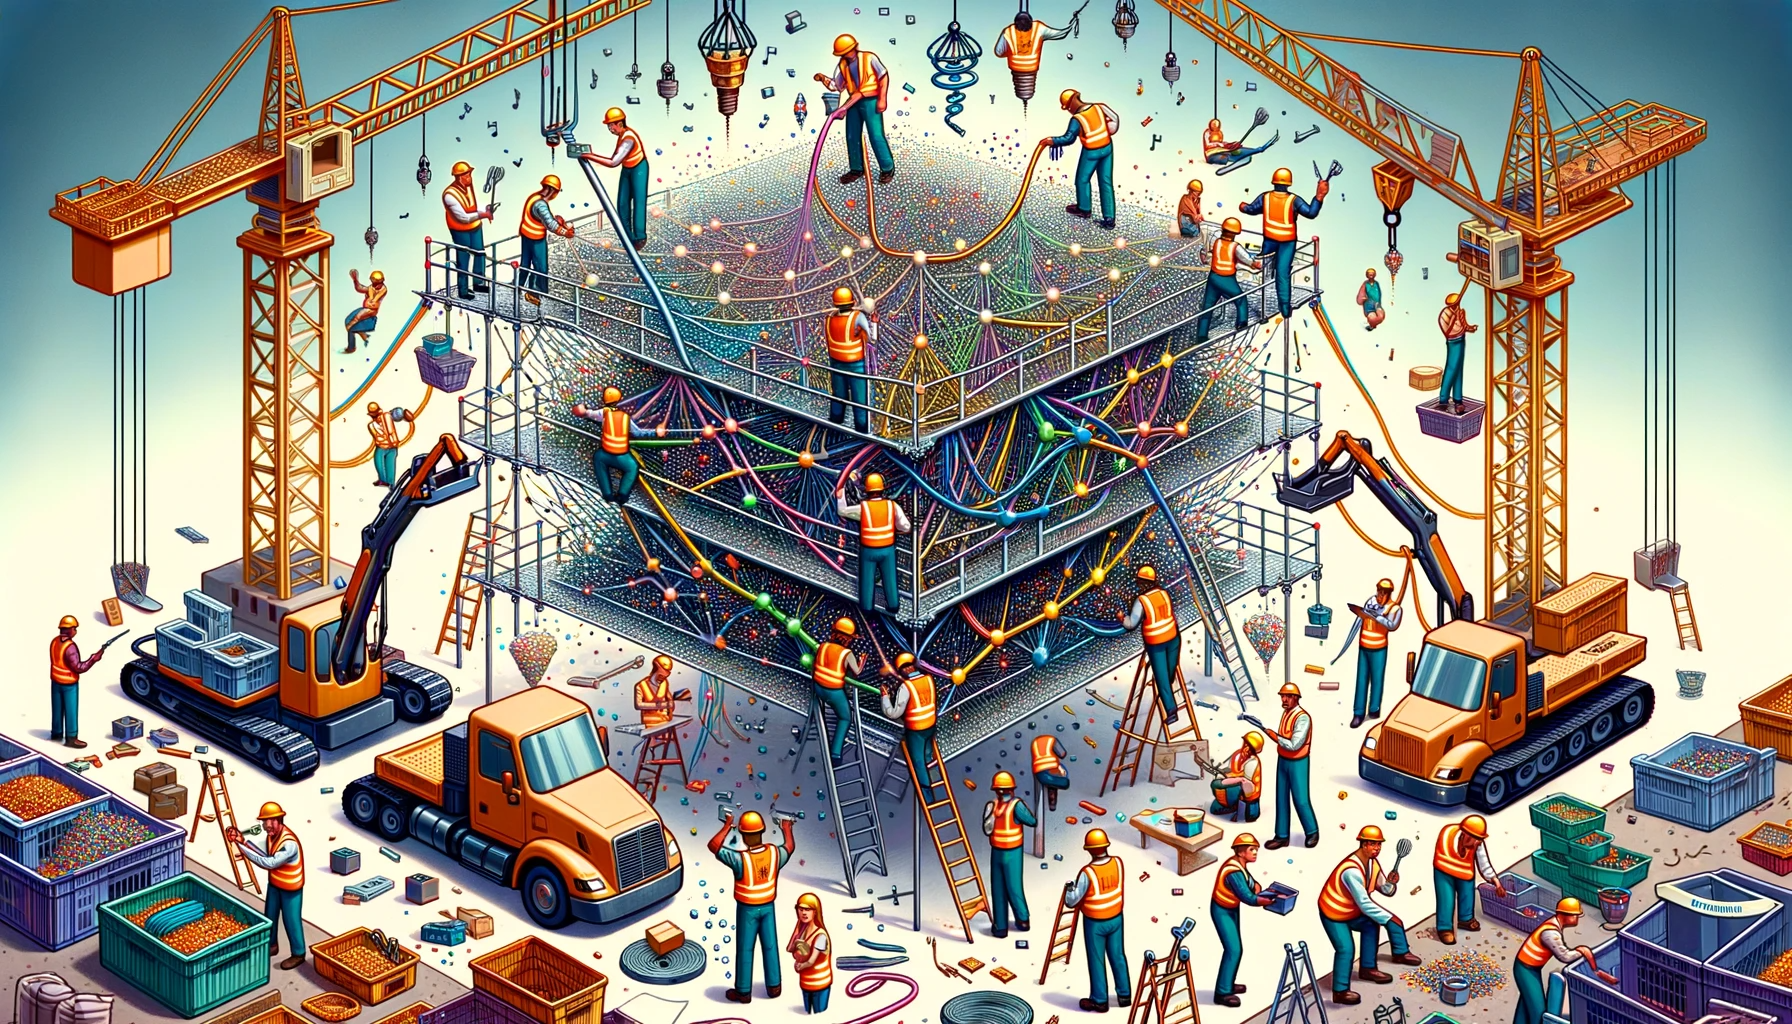
\includegraphics[keepaspectratio]{contents/vol1/optimizations/images/png/cover_model_optimizations.png}}

\section*{Purpose}\label{purpose}
\addcontentsline{toc}{section}{Purpose}

\markright{Purpose}

\emph{Why do the models that win benchmarks rarely become the models
that run in production?}

Training produced a capable model. But capability alone does not
guarantee deployability---Cloud, Edge, Mobile, and TinyML each impose
constraints that research benchmarks ignore. Research optimizes for
accuracy on held-out test sets; production optimizes for accuracy per
dollar, accuracy per watt, accuracy per millisecond. These objectives
diverge dramatically. The model that achieves state-of-the-art
performance typically does so by being larger, slower, and more
resource-intensive than any production constraint permits. A research
breakthrough that improves accuracy by 2\% while tripling compute
requirements is a step backward for deployment, where the original model
already exceeded accuracy requirements and the bottleneck was latency or
cost. This gap between research achievement and deployment viability is
not a failure of either community but a reflection of different
optimization targets. Model compression exists to bridge this gap---to
transform research artifacts into production assets by
\emph{systematically trading capabilities the deployment does not need
for constraints the deployment cannot violate}. The discipline is not
about making models smaller but about \emph{making the right models
possible}.

\begin{tcolorbox}[enhanced jigsaw, title=\textcolor{quarto-callout-tip-color}{\faLightbulb}\hspace{0.5em}{Learning Objectives}, leftrule=.75mm, colback=white, breakable, colframe=quarto-callout-tip-color-frame, opacityback=0, opacitybacktitle=0.6, rightrule=.15mm, toprule=.15mm, arc=.35mm, coltitle=black, bottomtitle=1mm, toptitle=1mm, titlerule=0mm, bottomrule=.15mm, colbacktitle=quarto-callout-tip-color!10!white, left=2mm]

\begin{itemize}
\tightlist
\item
  Explain the tripartite optimization framework: model representation
  (pruning), numerical precision (quantization), and architectural
  efficiency (distillation)
\item
  Compare quantization strategies in terms of memory reduction, energy
  consumption, and inference accuracy
\item
  Apply pruning techniques to reduce model parameters while quantifying
  the accuracy-sparsity trade-off
\item
  Implement knowledge distillation to transfer capabilities from large
  teacher models to efficient student architectures
\item
  Analyze hardware-aware design principles to align model operations
  with target platform capabilities
\item
  Design integrated optimization pipelines combining quantization,
  pruning, and distillation under resource constraints
\end{itemize}

\end{tcolorbox}

\section{Model Optimization
Fundamentals}\label{sec-model-compression-model-optimization-fundamentals-c0d7}

A 7-billion parameter language model requires 14 GB just to store its
weights in FP16. Your deployment target is a smartphone with 6 GB of RAM
shared across the operating system, applications, and your model.
\emph{The math does not work.} No amount of clever engineering changes
this arithmetic: 14 GB cannot fit in 6 GB. Yet users expect the model to
run: responsively, offline, without draining their battery in an hour.
The gap between what training produces and what deployment permits is
not a minor inconvenience but a five-orders-of-magnitude chasm that
defines the field of model compression.

Recall the \textbf{Silicon Contract}: every model architecture makes an
implicit agreement with the hardware about which resource it will
saturate: compute throughput, memory bandwidth, or memory capacity.
During training, this contract is negotiated upward. Researchers select
larger architectures, higher numerical precision, and deeper layers
because the training environment, typically a GPU cluster with hundreds
of gigabytes of memory, can afford those demands. In
\textbf{?@sec-ai-training}, we used Mixed Precision (FP16) to speed up
these training cycles while maintaining the ability to learn. Here, we
go further---to INT8 and beyond---for inference, where we trade the
ability to update weights for massive gains in execution efficiency.
Deployment reverses these priorities. The production environment is
smaller, power-constrained, and latency-sensitive, yet the model was
designed for an environment with none of those limitations. Model
compression is the systematic process of renegotiating that contract for
its new execution context: reducing memory footprint, computational
cost, and energy consumption while preserving the model's ability to
perform its task.

The scale of this renegotiation makes model optimization an engineering
discipline, not a collection of ad hoc tricks. A 175 billion parameter
model consumes over 350 GB in FP16 representation alone, yet a
smartphone provides 6 GB of RAM and a microcontroller offers 512 KB.
Bridging six orders of magnitude between what training produces and what
deployment permits requires systematic methods with predictable
trade-offs, not trial and error. Every optimization technique removes
something from the model, whether redundant parameters, numerical
precision, or architectural complexity, and the engineer must understand
exactly what is lost, what is preserved, and how these losses compose
when techniques are combined.

This chapter organizes these techniques along three complementary
dimensions. \emph{Structural optimization} removes redundancy from the
model itself: pruning eliminates parameters that contribute little to
output quality, knowledge distillation transfers a large model's learned
behavior into a smaller architecture, and neural architecture search
discovers designs that are inherently efficient. \emph{Precision
optimization} reduces the numerical bit-width of weights and
activations, for example converting 32-bit floating point values to
8-bit integers, which shrinks memory footprint and accelerates
arithmetic on hardware that supports lower-precision operations.
\emph{Hardware-level optimization} ensures that the resulting model
executes efficiently on the target processor by fusing operations to
reduce memory traffic and exploiting sparsity patterns that the hardware
can accelerate. These dimensions are not alternatives but layers in an
optimization stack. A practitioner deploying ResNet-50 to a mobile
device might prune 50\% of its filters, quantize the remaining weights
to INT8, and fuse batch normalization into convolution, with each
technique compounding the gains of the others.

Throughout this chapter, we ground each technique in concrete systems:
ResNet-50 and MobileNetV2 for vision workloads, transformer-based
language models for sequence tasks, and the DS-CNN keyword spotter for
TinyML deployment. These recurring models let us compare techniques
under consistent conditions, making the trade-offs between accuracy,
latency, memory, and energy tangible rather than abstract.

\phantomsection\label{callout-definitionux2a-1.1}
\begin{fbxSimple}{callout-definition}{Definition:}{Model Compression}
\phantomsection\label{callout-definition*-1.1}
\textbf{\emph{Model Compression}} is the systematic renegotiation of the
\textbf{Silicon Contract}. It transforms a research artifact, optimized
for \textbf{Information Density}, into a deployment artifact, optimized
for \textbf{Execution Efficiency}, by trading \textbf{Redundancy} and
\textbf{Precision} for \textbf{Latency}, \textbf{Memory}, and
\textbf{Energy} savings.

\end{fbxSimple}

\section{Optimization
Framework}\label{sec-model-compression-optimization-framework-9e21}

Model optimization is not a single technique but a \emph{framework} with
three complementary dimensions, each addressing different bottlenecks.
Figure~\ref{fig-3-sections} illustrates how these dimensions span from
pure software concerns to hardware-level execution.

\begin{figure}[htb]

\centering{

\pandocbounded{\includegraphics[keepaspectratio]{index_files/mediabag/7cb2f6aa6fa98c2fef6a2c7cb9472bdf88ee0619.pdf}}

}

\caption{\label{fig-3-sections}\textbf{Optimization Stack}: Model
optimization progresses through three layers: efficient model
representation, efficient numerics representation, and efficient
hardware implementation.}

\end{figure}%

\textbf{1. Efficient Model Representation:} Focuses on eliminating
redundancy in the model structure. Techniques like \textbf{pruning},
\textbf{knowledge distillation}, and \textbf{Neural Architecture Search
(NAS)} reduce the number of parameters or operations required,
addressing memory footprint and computational complexity at the
algorithmic level.

\textbf{2. Efficient Numerics Representation:} Optimizes how numerical
values are stored and processed. \textbf{Quantization} and
\textbf{mixed-precision} training reduce the bit-width of weights and
activations (e.g., from 32-bit floating point to 8-bit integers),
enabling faster execution and lower memory usage on specialized
hardware.

To understand \emph{why} numerics matter so deeply, consider the
\emph{physics of quantization} at the silicon level.

\phantomsection\label{callout-notebookux2a-1.2}
\begin{fbxSimple}{callout-notebook}{AI Engineer’s Notebook:}{The Physics of Quantization}
\phantomsection\label{callout-notebook*-1.2}
\emph{Why do we obsess over quantization?} Because the
\textbf{Energy-Movement Invariant} (\(E_{move} \gg E_{compute}\)) means
that in the physics of silicon, \textbf{bits represent energy} (see
\textbf{?@sec-system-foundations-numerical-representations-7b2f} for a
detailed comparison of FP32 vs.~INT8 energy costs).

According to the \textbf{Iron Law}
(\(T = \frac{D_{vol}}{BW} + \frac{O}{R_{peak} \cdot \eta} + L_{lat}\)),
reducing the bit-width of a weight has a quadratic effect on efficiency:

\begin{enumerate}
\def\labelenumi{\arabic{enumi}.}
\tightlist
\item
  \textbf{Memory Energy (\(D_{vol}\))}: Fetching a 32-bit float from
  DRAM costs \(\approx\) \textbf{640 pJ}. Fetching an 8-bit integer
  costs \(\approx\) \textbf{160 pJ}.
\item
  \textbf{Compute Energy (\(O\))}: A 32-bit FLOP costs \(\approx\)
  \textbf{3.7 pJ}. An 8-bit integer OP costs \(\approx\) \textbf{0.2
  pJ}.
\end{enumerate}

\begin{longtable}[]{@{}lrr@{}}
\toprule\noalign{}
\textbf{Operation} & \textbf{Bit-Width} & \textbf{Relative Energy} \\
\midrule\noalign{}
\endhead
\bottomrule\noalign{}
\endlastfoot
\textbf{Integer Add} & 8-bit & 1x \\
\textbf{Float Add} & 32-bit & 30x \\
\textbf{Memory Access} & 64-bit & \textbf{40,000x} \\
\end{longtable}

\textbf{For Inference}: Moving from FP32 to INT8 doesn't just save 4×
memory; it can reduce the \textbf{energy per inference} by nearly
\textbf{20×} if the hardware supports it.

This is the difference between a battery lasting 1 hour or 20 hours.

These same physics apply at datacenter scale: distributed training
systems use reduced precision to cut gradient communication overhead, a
topic covered in \textbf{?@sec-ai-training}.

\end{fbxSimple}

Figure~\ref{fig-quantization-free-lunch} visualizes this robustness,
showing the ``Free Lunch'' where reducing precision has minimal impact
on accuracy---until you hit the ``Cliff.''

\begin{figure}

\centering{

\pandocbounded{\includegraphics[keepaspectratio]{contents/vol1/optimizations/model_compression_files/figure-pdf/fig-quantization-free-lunch-output-1.pdf}}

}

\caption{\label{fig-quantization-free-lunch}\textbf{The Quantization
Free Lunch.} Model accuracy vs.~Bit-width. Most models exhibit a `Free
Lunch' plateau where reducing precision from FP32 to INT8 yields
\textless1\% accuracy loss. This robustness collapses at the
`Quantization Cliff' (typically 3-4 bits), where the noise overwhelms
the signal. Transformers (red) are generally more sensitive to
quantization outliers than CNNs (blue).}

\end{figure}%

These physics-level savings translate directly into deployment
capabilities. A model that cannot fit on a device at full precision may
run comfortably, and faster, when quantized. The following calculation
demonstrates the \emph{quantization speedup} for a concrete LLM
deployment scenario.

We call this phenomenon \emph{the quantization speedup}.

\phantomsection\label{callout-notebookux2a-1.3}
\begin{fbxSimple}{callout-notebook}{AI Engineer’s Notebook:}{The Quantization Speedup}
\phantomsection\label{callout-notebook*-1.3}
\textbf{Problem}: You want to deploy a 7B parameter LLM on a device with
16GB RAM. The weights are FP16 (2 bytes).

\textbf{The Math}:

\begin{enumerate}
\def\labelenumi{\arabic{enumi}.}
\tightlist
\item
  \textbf{Model Size}:
  \(7 \times 10^9 \text{ params} \times 2 \text{ bytes} = 14 \text{ GB}\).
\item
  \textbf{KV Cache}: Context window (4096 tokens) requires
  \(\approx 1 \text{ GB}\).
\item
  \textbf{Total Memory}: \(14 + 1 =\) 15 GB. This barely fits, leaving
  no room for OS or buffers.
\item
  \textbf{Bandwidth Cost}: Loading 14GB at 50 GB/s takes \textbf{280 ms}
  per token. That is 3.6 tokens/sec, too slow for chat.
\end{enumerate}

\textbf{The Fix (INT4)}:

\begin{enumerate}
\def\labelenumi{\arabic{enumi}.}
\tightlist
\item
  \textbf{Quantization}: Convert weights to 4-bit integers (0.5 bytes).
\item
  \textbf{New Size}: \(7 \times 10^9 \times 0\.5 =\) 3.5 GB.
\item
  \textbf{New Speed}: Loading 3.5GB takes \textbf{70 ms}. Speed jumps to
  \textbf{14 tokens/sec}.
\end{enumerate}

\textbf{The Conclusion}: Quantization is not just about ``fitting'' the
model; it is a \textbf{4x Linear Speedup} because LLM generation is
bandwidth-bound.

\end{fbxSimple}

\textbf{3. Efficient Hardware Implementation:} Ensures operations run
efficiently on target processors. Techniques like \textbf{operator
fusion}, \textbf{sparsity exploitation}, and \textbf{hardware-aware
scheduling} align computational patterns with hardware capabilities
(memory hierarchy, vector units) to maximize utilization and throughput.

These dimensions are interdependent. Pruning reduces complexity but may
require architectural changes for hardware efficiency. Quantization
reduces precision but impacts execution logic. The most effective
strategies combine techniques across all three layers. For practitioners
seeking immediate guidance on which techniques to apply,
Section~\ref{sec-model-compression-decision-framework-1896} provides a
decision framework that maps deployment constraints to specific
technique recommendations. The intervening sections provide the
technical foundation needed to apply that framework effectively.

Before examining deployment scenarios, we must understand these three
fundamental dimensions of model optimization: structural modifications
that change the network topology, precision adjustments that alter
numerical representation, and architectural innovations that redesign
computation patterns. The following sections detail each dimension; here
we preview how they combine in practice.

\section{Deployment
Context}\label{sec-model-compression-deployment-context-0d88}

Optimization requirements vary dramatically across deployment contexts.
What matters for cloud inference differs fundamentally from mobile or
embedded systems. Table~\ref{tbl-deployment-scenarios} summarizes the
key constraints across deployment environments.

\begin{longtable}[]{@{}
  >{\raggedright\arraybackslash}p{(\linewidth - 8\tabcolsep) * \real{0.2459}}
  >{\raggedright\arraybackslash}p{(\linewidth - 8\tabcolsep) * \real{0.1639}}
  >{\raggedleft\arraybackslash}p{(\linewidth - 8\tabcolsep) * \real{0.1803}}
  >{\raggedright\arraybackslash}p{(\linewidth - 8\tabcolsep) * \real{0.1475}}
  >{\raggedright\arraybackslash}p{(\linewidth - 8\tabcolsep) * \real{0.2623}}@{}}
\caption{\textbf{Deployment Constraints}: Each deployment context
imposes different optimization
priorities.}\label{tbl-deployment-scenarios}\tabularnewline
\toprule\noalign{}
\begin{minipage}[b]{\linewidth}\raggedright
\textbf{Context}
\end{minipage} & \begin{minipage}[b]{\linewidth}\raggedright
\textbf{Memory}
\end{minipage} & \begin{minipage}[b]{\linewidth}\raggedleft
\textbf{Latency}
\end{minipage} & \begin{minipage}[b]{\linewidth}\raggedright
\textbf{Power}
\end{minipage} & \begin{minipage}[b]{\linewidth}\raggedright
\textbf{Primary Goal}
\end{minipage} \\
\midrule\noalign{}
\endfirsthead
\toprule\noalign{}
\begin{minipage}[b]{\linewidth}\raggedright
\textbf{Context}
\end{minipage} & \begin{minipage}[b]{\linewidth}\raggedright
\textbf{Memory}
\end{minipage} & \begin{minipage}[b]{\linewidth}\raggedleft
\textbf{Latency}
\end{minipage} & \begin{minipage}[b]{\linewidth}\raggedright
\textbf{Power}
\end{minipage} & \begin{minipage}[b]{\linewidth}\raggedright
\textbf{Primary Goal}
\end{minipage} \\
\midrule\noalign{}
\endhead
\bottomrule\noalign{}
\endlastfoot
\textbf{Cloud} & 10s GB & 10-100ms & Flexible & Throughput, cost \\
\textbf{Mobile/Edge} & 100s MB--GB & 10-50ms & Watts & Size, latency \\
\textbf{TinyML} & KB--MB & 1-10ms & mW & Size, energy \\
\end{longtable}

\subsection{Deployment
Scenarios}\label{sec-model-compression-deployment-scenarios-70c9}

\textbf{Cloud inference} optimizes for throughput
(requests/second/dollar). Quantization enables serving more concurrent
requests; operator fusion reduces per-request latency
(\citeproc{ref-choudhary2020comprehensive}{Choudhary et al. 2020};
\citeproc{ref-dean2018new}{Dean, Patterson, and Young 2018}).
\textbf{Mobile and edge} deployments must fit device memory while
meeting real-time targets. A camera app processing 30 fps has 33ms per
frame, so any optimization reducing inference below this threshold
directly improves user experience.

\textbf{TinyML}\sidenote{\textbf{Microcontroller Constraints}:
Microcontrollers operate under severe constraints relative to servers
and modern accelerators, often with \emph{kilobytes to low megabytes} of
RAM and limited persistent storage. A practical mental model is that you
may have (10\^{}3) to (10\^{}6) bytes of memory available for the entire
pipeline, which is why ``model optimization'' is often a prerequisite
rather than an optional improvement in embedded deployments. } makes
optimization existential, not optional. A microcontroller with 256KB RAM
cannot run a 100MB model regardless of accuracy. The model must compress
below hardware limits or deployment is impossible
(\citeproc{ref-banbury2020benchmarking}{Banbury et al. 2020}). Even on
mobile devices with comparatively generous resources, a single
optimization technique can deliver a \emph{4x performance win} that
means the difference between a feature that ships and one that never
leaves the prototype stage.

\phantomsection\label{callout-exampleux2a-1.4}
\begin{fbxSimple}{callout-example}{Example:}{The 4x MobileNet Win}
\phantomsection\label{callout-example*-1.4}
\textbf{The Context}: A mobile app wants to add real-time ``Background
Blur'' to video calls. The feature requires a segmentation model running
at 30 FPS.

\textbf{The Bottleneck}: The unoptimized MobileNetV3 (FP32) runs at 8
FPS on mid-tier Android phones. It is too slow to ship.

\textbf{The Optimization}:

\begin{enumerate}
\def\labelenumi{\arabic{enumi}.}
\tightlist
\item
  \textbf{Quantization}: Converting weights to INT8 reduces size by 4x
  and uses the phone's DSP/NPU.
\item
  \textbf{Result}: Speed jumps to 35 FPS. Energy per frame drops by 3x.
\end{enumerate}

\textbf{The Business Value}: Compression didn't just ``optimize'' the
feature; it \textbf{enabled} it. Without INT8 quantization, the product
simply could not exist for the target market.

\end{fbxSimple}

Table~\ref{tbl-model-vs-device} quantifies this gap using the Lighthouse
models from \textbf{?@sec-ml-system-architecture}. The mismatch between
model requirements and device capabilities explains \emph{why}
compression is not optional for resource-constrained deployment: without
it, the models simply cannot run.

\begin{longtable}[]{@{}
  >{\raggedright\arraybackslash}p{(\linewidth - 10\tabcolsep) * \real{0.1158}}
  >{\raggedright\arraybackslash}p{(\linewidth - 10\tabcolsep) * \real{0.1526}}
  >{\raggedright\arraybackslash}p{(\linewidth - 10\tabcolsep) * \real{0.1526}}
  >{\raggedright\arraybackslash}p{(\linewidth - 10\tabcolsep) * \real{0.1895}}
  >{\raggedright\arraybackslash}p{(\linewidth - 10\tabcolsep) * \real{0.2000}}
  >{\raggedright\arraybackslash}p{(\linewidth - 10\tabcolsep) * \real{0.1895}}@{}}
\caption{\textbf{The Deployment Gap}: Model memory requirements compared
against typical device capacities. Even MobileNetV2 quantized to INT8
exceeds TinyML constraints by 7×, while the purpose-built DS-CNN keyword
spotter fits comfortably. Numbers in parentheses show how many times the
model exceeds device memory.}\label{tbl-model-vs-device}\tabularnewline
\toprule\noalign{}
\begin{minipage}[b]{\linewidth}\raggedright
\textbf{Model}
\end{minipage} & \begin{minipage}[b]{\linewidth}\raggedright
\textbf{Memory} \textbf{(Runtime)}
\end{minipage} & \begin{minipage}[b]{\linewidth}\raggedright
\textbf{Storage} \textbf{(Weights)}
\end{minipage} & \begin{minipage}[b]{\linewidth}\raggedright
\textbf{Cloud} \textbf{(\textasciitilde100 GB)}
\end{minipage} & \begin{minipage}[b]{\linewidth}\raggedright
\textbf{Mobile} \textbf{(\textasciitilde8 GB)}
\end{minipage} & \begin{minipage}[b]{\linewidth}\raggedright
\textbf{TinyML} \textbf{(\textasciitilde512 KB)}
\end{minipage} \\
\midrule\noalign{}
\endfirsthead
\toprule\noalign{}
\begin{minipage}[b]{\linewidth}\raggedright
\textbf{Model}
\end{minipage} & \begin{minipage}[b]{\linewidth}\raggedright
\textbf{Memory} \textbf{(Runtime)}
\end{minipage} & \begin{minipage}[b]{\linewidth}\raggedright
\textbf{Storage} \textbf{(Weights)}
\end{minipage} & \begin{minipage}[b]{\linewidth}\raggedright
\textbf{Cloud} \textbf{(\textasciitilde100 GB)}
\end{minipage} & \begin{minipage}[b]{\linewidth}\raggedright
\textbf{Mobile} \textbf{(\textasciitilde8 GB)}
\end{minipage} & \begin{minipage}[b]{\linewidth}\raggedright
\textbf{TinyML} \textbf{(\textasciitilde512 KB)}
\end{minipage} \\
\midrule\noalign{}
\endhead
\bottomrule\noalign{}
\endlastfoot
\textbf{DLRM} & 100 GB & 100 GB & ✓ & ✗ (12×) & ✓ \\
\textbf{GPT-2 XL} & 6 GB & 6 GB & ✓ & ✓ & ✓ \\
\textbf{ResNet-50} & 100 MB & 100 MB & ✓ & ✓ & ✓ \\
\textbf{MobileNetV2} & 14 MB & 14 MB & ✓ & ✓ & ✓ \\
\textbf{MobileNetV2 (INT8)} & 3.5 MB & 3.5 MB & ✓ & ✓ & ✓ \\
\textbf{DS-CNN (KWS)} & 500 KB & 500 KB & ✓ & ✓ & ✓ \\
\end{longtable}

Optimization also contributes to sustainable and accessible AI
deployment. Reducing a model's energy footprint is important as AI
workloads scale, helping mitigate the environmental impact of
large-scale ML training and inference
(\citeproc{ref-patterson2021carbon}{Patterson et al. 2021}). At the same
time, optimized models can expand the reach of machine learning,
supporting applications in low-resource environments, from rural
healthcare to autonomous systems operating in the field.

\subsection{Balancing
Trade-offs}\label{sec-model-compression-balancing-tradeoffs-6ae3}

The tension between accuracy and efficiency drives optimization
decisions across all dimensions. Increasing model capacity generally
enhances predictive performance while increasing computational cost,
resulting in slower, more resource-intensive inference. These
improvements introduce challenges related to memory
footprint\sidenote{Memory bandwidth (introduced in
\textbf{?@sec-introduction}) constrains how fast data moves between
memory and processors. For compression, bandwidth differences across
deployment targets matter: datacenter accelerators reach TB/s while
mobile devices achieve only tens of GB/s. Compression techniques that
reduce memory traffic often yield larger speedups than those that only
reduce computation. }, inference latency, power consumption, and
training efficiency. As machine learning systems are deployed across a
wide range of hardware platforms, balancing accuracy and efficiency
becomes a key challenge in model optimization.

This tension manifests differently across deployment contexts. Training
requires computational resources that scale with model size, while
inference demands strict latency and power constraints in real-time
applications. Navigating these trade-offs requires understanding where
each optimization technique falls on the \emph{compression-accuracy
Pareto frontier}.

\phantomsection\label{callout-perspectiveux2a-1.5}
\begin{fbxSimple}{callout-perspective}{Systems Perspective:}{The Compression-Accuracy Tradeoff Curve}
\phantomsection\label{callout-perspective*-1.5}
Optimization is a search for the \textbf{Pareto Frontier}.

\begin{itemize}
\tightlist
\item
  \textbf{Region 1: The Free Lunch}. Techniques like ``Operator Fusion''
  or ``Dead Code Elimination'' reduce latency without touching accuracy.
  Do these first.
\item
  \textbf{Region 2: The Efficient Trade}. Techniques like ``INT8
  Quantization'' might drop accuracy by 0.5\% but improve speed by
  400\%. This is usually a winning trade.
\item
  \textbf{Region 3: The Steep Drop}. Aggressive pruning (e.g., removing
  90\% of weights) might drop accuracy by 10\% to gain another 20\%
  speedup. This is the \textbf{danger zone} where the model becomes
  useless.
\end{itemize}

\textbf{Systems Rule}: Stop compressing when you hit the ``knee'' of the
curve, where the marginal loss in accuracy exceeds the marginal gain in
efficiency.

\end{fbxSimple}

Navigating this frontier requires understanding which techniques fall
into each region. Before examining specific optimization methods, verify
your intuition about these trade-offs.

\phantomsection\label{callout-checkpointux2a-1.6}
\begin{fbxSimple}{callout-checkpoint}{Checkpoint:}{The Efficiency Frontier}
\phantomsection\label{callout-checkpoint*-1.6}

Optimization is about trading one resource for another.

\textbf{Trade-offs}

\begin{itemize}
\tightlist
\item[$\square$]
  \textbf{Accuracy vs.~Cost}: Do you understand why removing 50\% of
  weights (Pruning) might drop accuracy by 1\%, but reducing precision
  (Quantization) to INT8 might drop it by 0.5\% while saving 4x memory?
\item[$\square$]
  \textbf{The ``Free Lunch''}: Can you identify optimizations like
  \textbf{Operator Fusion} that improve speed without hurting accuracy?
\end{itemize}

\textbf{Technique Selection}

\begin{itemize}
\tightlist
\item[$\square$]
  \textbf{Pruning}: When should you prune (reduce parameters)
  vs.~distill (train a smaller student)? (Hint: Pruning is for existing
  models; Distillation is for architectural changes).
\end{itemize}

\end{fbxSimple}

The following sections examine each optimization dimension in depth:
structural methods that modify what computations occur, precision
techniques that reduce numerical fidelity, and architectural approaches
that improve execution efficiency. After covering these techniques, we
provide a practical guide for selecting and combining them based on
deployment constraints.

\section{Structural Model Optimization
Methods}\label{sec-model-compression-structural-model-optimization-methods-8ed4}

We begin with the first dimension of our optimization framework:
\textbf{Efficient Model Representation}. This dimension addresses
\emph{what} to compute by modifying neural network structure and
parameters. Modern models often prioritize accuracy over efficiency,
containing excessive parameters that increase costs and slow inference.
This optimization addresses inefficiencies through two objectives:
eliminating redundancy (exploiting overparameterization where models
achieve similar performance with fewer parameters) and structuring
computations for efficient hardware execution through techniques like
gradient checkpointing\sidenote{\textbf{Gradient Checkpointing}: Memory
optimization technique that trades computation for memory by recomputing
intermediate activations during backpropagation instead of storing them.
Reduces memory usage by 20-50\% in transformer models, enabling larger
batch sizes or model sizes within same GPU memory. } and parallel
processing patterns\sidenote{\textbf{Parallel Processing in ML}:
Datacenter GPUs and other accelerators provide massive parallelism and
specialized matrix primitives compared to general-purpose CPUs. For
highly parallelizable ML workloads, accelerators can deliver
orders-of-magnitude higher throughput, although realized speedups depend
on kernel mix, memory behavior, and software stack. }.

The optimization challenge lies in balancing competing
constraints\sidenote{\textbf{Pareto Frontier}: Named after Italian
economist Vilfredo Pareto (1848-1923), who observed that 80\% of Italian
land was owned by 20\% of the population. In optimization, the Pareto
frontier represents solutions where improving one objective (speed)
requires sacrificing another (accuracy). EfficientNet traces this
frontier: B0 (77.1\%, 390M FLOPs) to B7 (84.4\%, 37B FLOPs).
Multi-objective NAS explicitly optimizes for Pareto-optimal
architectures. }, a direct manifestation of the Conservation of
Complexity thesis from \textbf{?@sec-part-foundations}: you cannot
destroy complexity, only move it. Pruning moves complexity from
parameters to the hardware's ability to exploit sparse patterns.
Quantization moves complexity from numerical precision to calibration
effort and potential accuracy loss. Knowledge distillation moves
complexity from inference compute to training compute. Aggressive
compression risks accuracy degradation that renders models unreliable
for production use, while insufficient optimization leaves models too
large or slow for target deployment environments. Selecting appropriate
techniques requires understanding where complexity should reside for
your specific deployment target.

Three key techniques address this challenge: pruning eliminates
low-impact parameters, knowledge distillation transfers capabilities to
smaller models, and NAS automates architecture design for specific
constraints. Each technique offers distinct optimization pathways while
maintaining model performance.

These three techniques represent distinct but complementary approaches
within our optimization framework. Pruning and knowledge distillation
reduce redundancy in existing models, while NAS addresses building
optimized architectures from the ground up. In many cases, they can be
combined to achieve even greater optimization.

\subsection{Pruning}\label{sec-model-compression-pruning-2b06}

Pruning\sidenote{\textbf{Pruning}: Borrowed from horticulture, where
gardeners prune branches to improve plant health and growth. The ML
metaphor fits precisely: just as removing unproductive branches
redirects resources to productive growth, removing low-magnitude weights
redirects computational resources to parameters that matter. The
technique dates to optimal brain damage
(\citeproc{ref-lecun1990optimal}{LeCun, Denker, and Solla 1989}), which
formalized the gardener's intuition with second-derivative analysis. }
directly addresses memory efficiency constraints by eliminating
redundant parameters. Modern neural networks are heavily
overparameterized, often containing far more weights than are strictly
necessary to solve a task. This redundancy allows us to remove a
significant fraction of weights without substantial performance
degradation. As we will explore in \textbf{?@sec-ai-acceleration},
specialized hardware can further exploit these sparse structures.

\phantomsection\label{callout-definitionux2a-1.7}
\begin{fbxSimple}{callout-definition}{Definition:}{Pruning}
\phantomsection\label{callout-definition*-1.7}
\textbf{\emph{Pruning}} is the sparsification of the \textbf{Parameter
Space}. It removes weights that contribute minimal information to the
\textbf{Loss Landscape}, converting dense matrices into sparse
structures to reduce \textbf{Memory Footprint} and, with specialized
hardware, \textbf{FLOPs}, at the cost of \textbf{Regularity}.

\end{fbxSimple}

The goal of pruning is to find a sparse version of the model parameters
\(\hat{W}\) that minimizes the increase in prediction error (loss) while
satisfying a fixed parameter budget \(k\). This is formalized as an
optimization problem:

\[
\min_{\hat{W}} \mathcal{L}(\hat{W}) \quad \text{subject to} \quad \|\hat{W}\|_0 \leq k
\]

where \(\|\hat{W}\|_0\) is the \textbf{L0-norm} (the count of non-zero
parameters). Since minimizing the L0-norm is
NP-hard\sidenote{\textbf{NP-hard}: From computational complexity theory,
``NP'' stands for ``nondeterministic polynomial time.'' A problem is
NP-hard if solving it in polynomial time would imply P=NP, widely
believed false. Finding the optimal sparse subnetwork requires examining
exponentially many subsets, making exact solutions infeasible for
networks with millions of parameters. }, we use
heuristics\sidenote{\textbf{Heuristic}: From Greek ``heuriskein'' (to
discover or find), the same root as ``eureka.'' Heuristics are practical
methods that find good solutions without guarantees of optimality.
Magnitude-based pruning assumes larger weights are more important, a
reasonable heuristic that works well empirically even though
counterexamples exist. } like \textbf{magnitude-based pruning}.
Listing~\ref{lst-pruning_example} demonstrates this approach, removing
weights with small absolute values to transform a dense weight matrix
into the sparse representation shown in Figure~\ref{fig-sparse-matrix}.

\begin{codelisting}

\caption{\label{lst-pruning_example}\textbf{Magnitude-Based Pruning}:
Removes weights below a threshold to create sparse matrices, reducing
the number of nonzero parameters from 9 to 4 (\(k=4\)).}

\centering{

\begin{Shaded}
\begin{Highlighting}[]
\ImportTok{import}\NormalTok{ torch}

\CommentTok{\# Original dense weight matrix}
\NormalTok{weights }\OperatorTok{=}\NormalTok{ torch.tensor(}
\NormalTok{    [[}\FloatTok{0.8}\NormalTok{, }\FloatTok{0.1}\NormalTok{, }\OperatorTok{{-}}\FloatTok{0.7}\NormalTok{], [}\FloatTok{0.05}\NormalTok{, }\OperatorTok{{-}}\FloatTok{0.9}\NormalTok{, }\FloatTok{0.03}\NormalTok{], [}\OperatorTok{{-}}\FloatTok{0.6}\NormalTok{, }\FloatTok{0.02}\NormalTok{, }\FloatTok{0.4}\NormalTok{]]}
\NormalTok{)}

\CommentTok{\# Simple magnitude{-}based pruning: keep only the 4 largest weights}
\NormalTok{threshold }\OperatorTok{=} \FloatTok{0.5}
\NormalTok{mask }\OperatorTok{=}\NormalTok{ torch.}\BuiltInTok{abs}\NormalTok{(weights) }\OperatorTok{\textgreater{}=}\NormalTok{ threshold}
\NormalTok{pruned\_weights }\OperatorTok{=}\NormalTok{ weights }\OperatorTok{*}\NormalTok{ mask}

\BuiltInTok{print}\NormalTok{(}\StringTok{"Original:"}\NormalTok{, weights)}
\BuiltInTok{print}\NormalTok{(}\StringTok{"Pruned (4 non{-}zeros):"}\NormalTok{, pruned\_weights)}
\end{Highlighting}
\end{Shaded}

}

\end{codelisting}%

\begin{figure}[htb]

\centering{

\pandocbounded{\includegraphics[keepaspectratio]{index_files/mediabag/06a0aa5679a9d9c1015a4a00b628207b390cb1b2.pdf}}

}

\caption{\label{fig-sparse-matrix}\textbf{Sparse Matrix Transformation}:
Pruning removes small-magnitude weights (shown as white/zero in the
right matrix) while preserving large-magnitude weights (shown in color),
creating a sparse representation that reduces memory usage while
maintaining model accuracy.}

\end{figure}%

To make pruning computationally feasible, practical methods often
replace the hard L0 constraint with soft regularization like L1-norm
(\(\lambda \| W \|_1\)), which encourages small values that can later be
thresholded to zero. Practitioners typically use \textbf{iterative
pruning}, where parameters are removed in successive steps interleaved
with fine-tuning to recover lost accuracy
(\citeproc{ref-gale2020sparse}{Gale, Elsen, and Hooker 2019a};
\citeproc{ref-blalock2020state}{Labarge, n.d.}).

\subsubsection{Target
Structures}\label{sec-model-compression-target-structures-c474}

Pruning methods vary based on which structures within a neural network
are removed. The primary targets include neurons, channels, and layers,
each with distinct implications for the model's architecture and
performance.

\begin{itemize}
\item
  \textbf{Neuron pruning} removes entire neurons along with their
  associated weights and biases, reducing the width of a layer. This
  technique is often applied to fully connected layers.
\item
  \textbf{Channel pruning} (or filter pruning), commonly used in
  convolutional neural networks, eliminates entire channels or filters.
  This reduces the depth of feature maps, which impacts the network's
  ability to extract certain features. Channel pruning proves valuable
  in image-processing tasks where computational efficiency is a
  priority.
\item
  \textbf{Layer pruning} removes entire layers from the network,
  significantly reducing depth. While this approach can yield
  significant efficiency gains, it requires careful balance to ensure
  the model retains sufficient capacity to capture complex patterns.
\end{itemize}

Figure~\ref{fig-channel-layer-pruning} illustrates the differences
between channel pruning and layer pruning. When a channel is pruned, the
model's architecture must be adjusted to accommodate the structural
change. Specifically, the number of input channels in subsequent layers
must be modified, requiring alterations to the depths of the filters
applied to the layer with the removed channel. In contrast, layer
pruning removes all channels within a layer, necessitating more
significant architectural modifications. In this case, connections
between remaining layers must be reconfigured to bypass the removed
layer. Regardless of the pruning approach, fine-tuning is important to
adapt the remaining network and restore performance.

\begin{figure}[htb]

\centering{

\pandocbounded{\includegraphics[keepaspectratio]{index_files/mediabag/191f3fefb92b78746aed86aea6f86dc182d5fcb5.pdf}}

}

\caption{\label{fig-channel-layer-pruning}\textbf{Channel vs.~Layer
Pruning.} Channel pruning adjusts filter sizes within layers, while
layer pruning removes entire layers and necessitates reconnection of
remaining network components. These approaches reduce model size and
computational cost, but require fine-tuning to mitigate performance loss
due to reduced model capacity.}

\end{figure}%

\subsubsection{Unstructured
Pruning}\label{sec-model-compression-unstructured-pruning-280e}

Unstructured pruning removes individual weights while preserving the
overall network architecture. During training, some connections become
redundant, contributing little to the final computation. Pruning these
weak connections reduces memory requirements while preserving most of
the model's accuracy.

The mathematical foundation for unstructured pruning clarifies how
sparsity is systematically introduced. Unstructured pruning introduces
sparsity into the weight matrices of a neural network. Let
\(W \in \mathbb{R}^{m \times n}\) represent a weight matrix in a given
layer of a network. Pruning removes a subset of weights by applying a
binary mask \(M \in \{0,1\}^{m \times n}\), yielding a pruned weight
matrix: \[
\hat{W} = M \odot W
\] where \(\odot\) represents the element-wise Hadamard product. The
mask \(M\) is constructed based on a pruning criterion, typically weight
magnitude. A common approach is magnitude-based pruning, which removes a
fraction \(s\) of the lowest-magnitude weights. This is achieved by
defining a threshold \(\tau\) such that: \[
M_{i,j} =
\begin{cases}
1, & \text{if } |W_{i,j}| > \tau \\
0, & \text{otherwise}
\end{cases}
\] where \(\tau\) is chosen to ensure that only the largest \((1 - s)\)
fraction of weights remain. This method assumes that larger-magnitude
weights contribute more to the network's function, making them
preferable for retention.

The primary advantage of unstructured pruning is memory efficiency. By
reducing the number of nonzero parameters, pruned models require less
storage, which benefits deployment to embedded or mobile devices with
limited memory.

However, unstructured pruning does not necessarily improve computational
efficiency on modern machine learning hardware. Standard GPUs and TPUs
are optimized for dense matrix multiplications, and a sparse weight
matrix often cannot fully utilize hardware acceleration unless
specialized sparse computation kernels are available. Unstructured
pruning therefore primarily benefits model storage rather than inference
acceleration, and it does not alter the structural organization of the
network.

\subsubsection{Structured
Pruning}\label{sec-model-compression-structured-pruning-b651}

Where unstructured pruning removes individual weights, structured
pruning (\citeproc{ref-li2017pruning}{H. Li et al.
2017})\sidenote{\textbf{Structured Pruning}: Removing entire
filters/channels rather than individual weights, enabling immediate
hardware speedups without sparse computation support. ResNet-34 filter
pruning achieves 50\% FLOP reduction with 1.0\% accuracy loss;
MobileNetV2 channel pruning yields 3.2× faster ARM inference at 96.5\%
accuracy. Importance metrics include magnitude, gradient, and Taylor
expansion. } eliminates entire computational units: neurons, filters,
channels, or layers. This approach produces smaller dense models that
map directly to modern machine learning accelerators. Because the
resulting architecture remains fully dense, structured pruning leads to
more efficient inference on general-purpose hardware than unstructured
pruning, which requires specialized execution kernels to exploit its
sparse weight matrices.

Structured pruning is motivated by the observation that not all neurons,
filters, or layers contribute equally to a model's predictions. Some
units primarily carry redundant or low-impact information, and removing
them does not significantly degrade model performance. Identifying which
structures can be pruned while preserving accuracy remains the core
challenge.

Hardware-aware pruning strategies, such as N:M structured sparsity,
enforce specific patterns (e.g., ensuring 2 out of every 4 weights are
zero) to align with specialized accelerator capabilities. The hardware
implementation details of these patterns, including how they leverage
sparse tensor cores, are covered in \textbf{?@sec-ai-acceleration}.

Figure~\ref{fig-structured-unstructured} illustrates the key differences
between unstructured and structured pruning. On the left, unstructured
pruning removes individual weights (depicted as dashed connections),
creating a sparse weight matrix. This can disrupt the original network
structure, as shown in the fully connected network where certain
connections have been randomly pruned. While this reduces the number of
active parameters, the resulting sparsity requires specialized execution
kernels to fully utilize computational benefits.

\begin{figure}[htb]

\centering{

\pandocbounded{\includegraphics[keepaspectratio]{index_files/mediabag/a17bac5eb7216e6693f669dbfb247542aa7ee1b9.pdf}}

}

\caption{\label{fig-structured-unstructured}\textbf{Unstructured
vs.~Structured Pruning.} Unstructured pruning (left) achieves sparsity
by removing individual weights, requiring specialized hardware, while
structured pruning (middle, right) removes entire neurons or filters,
preserving network structure for standard hardware acceleration. Source:
(\citeproc{ref-qi2021efficient}{Qi et al. 2021}).}

\end{figure}%

In contrast, structured pruning (depicted in the middle and right
sections of Figure~\ref{fig-structured-unstructured}) removes entire
neurons or filters while preserving the network's overall structure. In
the middle section, a pruned fully connected network retains its fully
connected nature but with fewer neurons. On the right, structured
pruning is applied to a CNN by removing convolutional kernels or entire
channels (dashed squares). This method maintains the CNN's core
convolutional operations while reducing the computational load, making
it more compatible with hardware accelerators.

A common approach to structured pruning is magnitude-based pruning,
where entire neurons or filters are removed based on the magnitude of
their associated weights. The intuition is that parameters with smaller
magnitudes contribute less to the model's output, making them candidates
for elimination. The importance of a neuron or filter is measured using
a norm function, such as the \(\ell_1\)-norm or \(\ell_2\)-norm, applied
to the weights associated with that unit. If the norm falls below a
predefined threshold, the corresponding neuron or filter is pruned. This
method is straightforward to implement and requires no additional
computational overhead beyond computing norms across layers.

Another strategy is activation-based pruning, which evaluates the
average activation values of neurons or filters over a dataset. Neurons
that consistently produce low activations contribute less information to
the network's decision process and can be safely removed. This method
captures the dynamic behavior of the network rather than relying solely
on static weight values. Activation-based pruning requires profiling the
model over a representative dataset to estimate the average activation
magnitudes before making pruning decisions.

Gradient-based pruning uses information from the model's training
process to identify less significant neurons or filters. The key idea is
that units with smaller gradient magnitudes contribute less to reducing
the loss function, making them less important for learning. By ranking
neurons based on their gradient values, structured pruning can remove
those with the least impact on model optimization. Unlike
magnitude-based or activation-based pruning, which rely on static
properties of the trained model, gradient-based pruning requires access
to gradient computations and is typically applied during training rather
than as a post-processing step.

Each of these methods presents trade-offs in terms of computational
complexity and effectiveness. Magnitude-based pruning is computationally
inexpensive and easy to implement but does not account for how neurons
behave across different data distributions. Activation-based pruning
provides a more data-driven pruning approach but requires additional
computations to estimate neuron importance. Gradient-based pruning
leverages training dynamics but may introduce additional complexity if
applied to large-scale models. The choice of method depends on the
specific constraints of the target deployment environment and the
performance requirements of the pruned model.

\subsubsection{Dynamic
Pruning}\label{sec-model-compression-dynamic-pruning-adee}

Traditional pruning methods, whether unstructured or structured,
typically involve static pruning: parameters are permanently removed
after training or at fixed intervals during training. This approach
assumes that parameter importance is fixed, which is not always the
case. Dynamic pruning instead adapts pruning decisions based on the
input data or training dynamics, allowing the model to adjust its
structure in real time.

Dynamic pruning can be implemented using runtime sparsity techniques,
where the model actively determines which parameters to utilize based on
input characteristics. Activation-conditioned pruning exemplifies this
approach by selectively deactivating neurons or channels that exhibit
low activation values for specific inputs
(\citeproc{ref-dynamicpruning2023}{J. Hu et al. 2023}). This method
introduces input-dependent sparsity patterns, effectively reducing the
computational workload during inference without permanently modifying
the model architecture.

For instance, consider a convolutional neural network processing images
with varying complexity. During inference of a simple image containing
mostly uniform regions, many convolutional filters may produce
negligible activations. Dynamic pruning identifies these low-impact
filters and temporarily excludes them from computation, improving
efficiency while maintaining accuracy for the current input. This
adaptive behavior is particularly advantageous in latency-sensitive
applications, where computational resources must be allocated
judiciously based on input complexity. \textbf{?@sec-benchmarking-ai}
presents measurement strategies for evaluating such efficiency gains.

Another class of dynamic pruning operates during training, where
sparsity is gradually introduced and adjusted throughout the
optimization process. Methods such as gradual magnitude pruning start
with a dense network and progressively increase the fraction of pruned
parameters as training progresses. Instead of permanently removing
parameters, these approaches allow the network to recover from
pruning-induced capacity loss by regrowing connections that prove to be
important in later stages of training.

Dynamic pruning presents several advantages over static pruning. It
allows models to adapt to different workloads, improving efficiency
while maintaining accuracy. Where static pruning risks over-pruning and
degrading performance, dynamic pruning provides a mechanism for
selectively reactivating parameters when necessary. The cost of this
flexibility is additional computational overhead, as pruning decisions
must be made in real time during training or inference. This complexity
makes dynamic pruning harder to integrate into standard machine learning
pipelines, requiring sophisticated production deployment strategies and
monitoring frameworks covered in
\textbf{?@sec-machine-learning-operations-mlops}.

Despite these challenges, dynamic pruning proves useful in edge
computing and efficient AI contexts discussed in
\textbf{?@sec-introduction}, where resource constraints and real-time
efficiency requirements vary across inputs.

\subsubsection{Pruning
Trade-offs}\label{sec-model-compression-pruning-tradeoffs-c139}

Pruning techniques offer different trade-offs in terms of memory
efficiency, computational efficiency, accuracy retention, hardware
compatibility, and implementation complexity. The choice of pruning
strategy depends on the specific constraints of the machine learning
system and the deployment environment, integrating with operational
considerations from \textbf{?@sec-machine-learning-operations-mlops}.

Unstructured pruning effectively reduces model size and memory footprint
by removing individual weights while keeping the overall model
architecture intact. However, since machine learning accelerators are
optimized for dense matrix operations, unstructured pruning does not
always translate to significant computational speed-ups unless
specialized sparse execution kernels are used.

Structured pruning, in contrast, eliminates entire neurons, channels, or
layers, leading to a more hardware-friendly model. This technique
provides direct computational savings, as it reduces the number of
floating-point operations (FLOPs)\sidenote{\textbf{FLOPs (Floating-Point
Operations)}: Computational complexity metric counting multiply-add
operations. ResNet-50 requires approximately 4.1 billion FLOPs per
inference (\citeproc{ref-he2016deep}{K. He et al. 2016}), GPT-3 training
required an estimated 3.14E23 FLOPs
(\citeproc{ref-patterson2021carbon}{Patterson et al. 2021}). Modern GPUs
achieve 100-300 TFLOPS (trillion FLOPs/second), making FLOP reduction
important for efficiency. } required during inference.

The downside is that modifying the network structure can lead to a
greater accuracy drop, requiring careful fine-tuning to recover lost
performance.

Dynamic pruning introduces adaptability into the pruning process by
adjusting which parameters are pruned at runtime based on input data or
training dynamics. This allows for a better balance between accuracy and
efficiency, as the model retains the flexibility to reintroduce
previously pruned parameters if needed. However, dynamic pruning
increases implementation complexity, as it requires additional
computations to determine which parameters to prune on-the-fly.

Table~\ref{tbl-pruning} formalizes these comparisons.

\begin{longtable}[]{@{}
  >{\raggedright\arraybackslash}p{(\linewidth - 6\tabcolsep) * \real{0.1057}}
  >{\raggedright\arraybackslash}p{(\linewidth - 6\tabcolsep) * \real{0.3780}}
  >{\raggedright\arraybackslash}p{(\linewidth - 6\tabcolsep) * \real{0.2967}}
  >{\raggedright\arraybackslash}p{(\linewidth - 6\tabcolsep) * \real{0.2195}}@{}}
\caption{\textbf{Pruning Strategies}: Unstructured, structured, and
dynamic pruning each modify model weights differently, impacting both
model size and computational efficiency. Unstructured pruning offers the
greatest compression but requires specialized hardware, while dynamic
pruning adapts to input data for a balance between accuracy and resource
usage.}\label{tbl-pruning}\tabularnewline
\toprule\noalign{}
\begin{minipage}[b]{\linewidth}\raggedright
\textbf{Aspect}
\end{minipage} & \begin{minipage}[b]{\linewidth}\raggedright
\textbf{Unstructured Pruning}
\end{minipage} & \begin{minipage}[b]{\linewidth}\raggedright
\textbf{Structured Pruning}
\end{minipage} & \begin{minipage}[b]{\linewidth}\raggedright
\textbf{Dynamic Pruning}
\end{minipage} \\
\midrule\noalign{}
\endfirsthead
\toprule\noalign{}
\begin{minipage}[b]{\linewidth}\raggedright
\textbf{Aspect}
\end{minipage} & \begin{minipage}[b]{\linewidth}\raggedright
\textbf{Unstructured Pruning}
\end{minipage} & \begin{minipage}[b]{\linewidth}\raggedright
\textbf{Structured Pruning}
\end{minipage} & \begin{minipage}[b]{\linewidth}\raggedright
\textbf{Dynamic Pruning}
\end{minipage} \\
\midrule\noalign{}
\endhead
\bottomrule\noalign{}
\endlastfoot
\textbf{What is removed?} & Individual weights in the model & Entire
neurons, channels, filters, or layers & Adjusts pruning based on runtime
conditions \\
\textbf{Model structure} & Sparse weight matrices; original architecture
remains unchanged & Model architecture is modified; pruned layers are
fully removed & Structure adapts dynamically \\
\textbf{Impact on memory} & Reduces model storage by eliminating nonzero
weights & Reduces model storage by removing entire components & Varies
based on real-time pruning \\
\textbf{Impact on computation} & Limited; dense matrix operations still
required unless specialized sparse computation is used & Directly
reduces FLOPs and speeds up inference & Balances accuracy and efficiency
dynamically \\
\textbf{Hardware compatibility} & Sparse weight matrices require
specialized execution support for efficiency & Works efficiently with
standard deep learning hardware & Requires adaptive inference engines \\
\textbf{Fine-tuning required?} & Often necessary to recover accuracy
after pruning & More likely to require fine-tuning due to larger
structural modifications & Adjusts dynamically, reducing the need for
fine-tuning \\
\textbf{Use cases} & Memory-efficient model compression for cloud
deployment & Real-time inference optimization, mobile/edge AI, and
efficient training & Adaptive AI applications, real-time systems \\
\end{longtable}

\subsubsection{Pruning
Strategies}\label{sec-model-compression-pruning-strategies-d1ce}

Beyond the broad categories of unstructured, structured, and dynamic
pruning, different pruning workflows can impact model efficiency and
accuracy retention. Two widely used pruning strategies are iterative
pruning and one-shot pruning, each with distinct benefits and
trade-offs.

\paragraph{Iterative
Pruning}\label{sec-model-compression-iterative-pruning-6c58}

Iterative pruning removes structure gradually through multiple cycles of
pruning followed by fine-tuning. During each cycle, the algorithm
removes a small subset of structures based on predefined importance
metrics. The model then undergoes fine-tuning to adapt to these
structural modifications before proceeding to the next pruning
iteration. This gradual approach helps prevent sudden drops in accuracy
while allowing the network to progressively adjust to reduced
complexity.

Figure~\ref{fig-iterative-pruning} illustrates this process using a
convolutional neural network where six channels are pruned. Rather than
removing all channels simultaneously, iterative pruning eliminates two
channels per iteration over three cycles. Following each pruning step,
the model undergoes fine-tuning to recover performance. The first
iteration, which removes two channels, results in an accuracy decrease
from 0.995 to 0.971, but subsequent fine-tuning restores accuracy to
0.992. After completing two additional pruning-tuning cycles, the final
model achieves 0.991 accuracy, which represents only a 0.4\% reduction
from the original, while operating with 27\% fewer channels. By
distributing structural modifications across multiple iterations, the
network maintains its performance capabilities while achieving improved
computational efficiency.

\begin{figure}[htb]

\centering{

\pandocbounded{\includegraphics[keepaspectratio]{index_files/mediabag/4df0c69cd7c1e002d0307b90644b41007395ad3c.pdf}}

}

\caption{\label{fig-iterative-pruning}\textbf{Iterative Pruning
Performance}: Three rows depict successive prune-then-fine-tune cycles,
each removing two of the original 22 channels. Accuracy drops from 0.995
to 0.971 after the first prune, recovers to 0.992 after fine-tuning, and
settles at 0.991 after all three cycles, a 0.4\% loss with 27\% fewer
channels.}

\end{figure}%

\paragraph{One-shot
Pruning}\label{sec-model-compression-oneshot-pruning-bad9}

One-shot pruning removes multiple architectural components in a single
step, followed by an extensive fine-tuning phase to recover model
accuracy. This aggressive approach compresses the model quickly but
risks greater accuracy degradation, as the network must adapt to
significant structural changes simultaneously.

Consider applying one-shot pruning to the same network from the
iterative pruning example. Instead of removing two channels at a time
over multiple iterations, one-shot pruning eliminates all six channels
simultaneously, as illustrated in Figure~\ref{fig-oneshot-pruning}.
Removing 27\% of the network's channels simultaneously causes the
accuracy to drop significantly, from 0.995 to 0.914. Even after
fine-tuning, the network only recovers to an accuracy of 0.943, which is
a 5\% degradation from the original unpruned network. While both
iterative and one-shot pruning ultimately produce identical network
structures, the gradual approach of iterative pruning better preserves
model performance.

\begin{figure}[htb]

\centering{

\pandocbounded{\includegraphics[keepaspectratio]{index_files/mediabag/03bc2df29f8203d136d58fee6ac18b3c964aabcd.pdf}}

}

\caption{\label{fig-oneshot-pruning}\textbf{One-Shot Pruning Impact}:
All six channels (27\%) are removed simultaneously, causing accuracy to
drop from 0.995 to 0.914. Fine-tuning recovers only to 0.943, a 5\%
degradation compared to the 0.4\% loss from iterative pruning,
illustrating why gradual removal preserves accuracy more effectively.}

\end{figure}%

The choice of pruning strategy depends on several interrelated factors.
The desired level of parameter reduction, or sparsity target, directly
impacts strategy selection: higher reduction targets often necessitate
iterative approaches to maintain accuracy, while moderate sparsity goals
may be achievable through simpler one-shot methods.

Available computational resources also influence strategy choice.
Iterative pruning demands significant resources for multiple fine-tuning
cycles, whereas one-shot approaches require fewer resources but may
sacrifice accuracy. Applications with strict accuracy requirements
typically benefit from gradual, iterative pruning, while use cases with
more flexible performance constraints may accommodate more aggressive
one-shot approaches.

Development timeline matters as well. One-shot methods enable faster
deployment when time is limited, though iterative approaches generally
achieve superior results given sufficient optimization periods. Target
platform capabilities further influence strategy selection, as certain
hardware architectures better support specific sparsity patterns, making
particular pruning approaches more advantageous for deployment.

\subsubsection{Lottery Ticket
Hypothesis}\label{sec-model-compression-lottery-ticket-hypothesis-a5bd}

Pruning is widely used to reduce the size and computational cost of
neural networks, but the process of determining which parameters to
remove is not always straightforward. While traditional pruning methods
eliminate weights based on magnitude, structure, or dynamic conditions,
recent research suggests that pruning is not just about reducing
redundancy. It may also reveal inherently efficient subnetworks that
exist within the original model.

This perspective leads to the Lottery Ticket
Hypothesis\sidenote{\textbf{Lottery Ticket Hypothesis}: Named for the
intuition that training a large network is like buying many lottery
tickets: most lose, but a few ``winning tickets'' (sparse subnetworks
with lucky initializations) can win (train to full accuracy) on their
own. Frankle and Carbin (\citeproc{ref-frankle2019lottery}{Frankle and
Carbin 2019}) showed ResNet-18 subnetworks at 10-20\% original size
achieve 93.2\% vs.~94.1\% accuracy. BERT-base winning tickets retain
97\% performance with 90\% fewer parameters. } (LTH), which challenges
conventional pruning workflows by proposing that within large neural
networks, there exist small, well-initialized subnetworks (``winning
tickets'') that can achieve comparable accuracy to the full model when
trained in isolation. Rather than viewing pruning as a post-training
compression step, LTH suggests it can serve as a discovery mechanism to
identify these efficient subnetworks early in training.

LTH is validated through an iterative pruning process, illustrated in
Figure~\ref{fig-winning-ticket}. A large network is first trained to
convergence. The lowest-magnitude weights are then pruned, and the
remaining weights are reset to their original initialization rather than
being re-randomized. This process is repeated iteratively, gradually
reducing the network's size while preserving performance. After multiple
iterations, the remaining subnetwork (the ``winning ticket'') proves
capable of training to the same or higher accuracy as the original full
model.

\begin{figure}[htb]

\centering{

\pandocbounded{\includegraphics[keepaspectratio]{index_files/mediabag/ada6c6fd73c2f507214bb8e7073a96409cb01895.pdf}}

}

\caption{\label{fig-winning-ticket}\textbf{Lottery Ticket Iteration
Cycle.} A dense network is trained to convergence, the
smallest-magnitude weights are pruned, and the surviving weights are
reset to their original initialization. Repeating this cycle
progressively identifies a sparse subnetwork (the winning ticket) that
matches or exceeds the full model's accuracy.}

\end{figure}%

The implications of the Lottery Ticket Hypothesis extend beyond
conventional pruning. Instead of training large models and pruning them
later, LTH suggests that compact, high-performing subnetworks could be
trained directly from the start, eliminating the need for
overparameterization. This insight challenges the traditional assumption
that model size is necessary for effective learning. It also emphasizes
the importance of initialization, as winning tickets only retain their
performance when reset to their original weight values, raising deeper
questions about how initialization shapes a network's learning
trajectory.

The hypothesis further reinforces the effectiveness of iterative pruning
over one-shot pruning. Gradually refining the model structure allows the
network to adapt at each stage, preserving accuracy more effectively
than removing large portions of the model in a single step. This process
aligns well with practical pruning strategies used in deployment, where
preserving accuracy while reducing computation is important.

Despite its promise, applying LTH in practice remains computationally
expensive because identifying winning tickets requires multiple cycles
of pruning and retraining. Ongoing research explores whether winning
subnetworks can be detected early without full training, potentially
leading to more efficient sparse training techniques. If such methods
become practical, LTH could fundamentally reshape how machine learning
models are trained, shifting the focus from pruning large networks after
training to discovering and training only the important components from
the beginning.

While LTH presents a compelling theoretical perspective on pruning,
practical implementations rely on established framework-level tools to
integrate structured and unstructured pruning techniques.

\subsubsection{Pruning in
Practice}\label{sec-model-compression-pruning-practice-bb32}

Modern machine learning frameworks provide dedicated APIs to automate
the pruning and fine-tuning workflow.

In \textbf{PyTorch}, the \texttt{torch.nn.utils.prune} module provides a
flexible interface for pruning individual layers or entire models. Users
can apply unstructured pruning (e.g., \texttt{l1\_unstructured}) or
structured pruning (e.g., \texttt{ln\_structured}) with just a few lines
of code. PyTorch uses ``masks'' to handle pruning: the original
parameters are preserved, but a binary mask is multiplied element-wise
during the forward pass. To realize actual memory savings for
deployment, these masks must be ``permanently'' applied using
\texttt{prune.remove(module,\ \textquotesingle{}weight\textquotesingle{})}.

\textbf{TensorFlow} implements pruning through the \textbf{TensorFlow
Model Optimization Toolkit (TF-MOT)}. Unlike PyTorch's post-training
approach, TF-MOT often integrates pruning into the training process
itself. By using \texttt{prune\_low\_magnitude}, the framework gradually
increases sparsity during training, allowing the model to adapt its
remaining weights to the sparse structure in real-time.

These trade-offs become concrete when examining real-world deployments.
Several high-profile models have successfully integrated pruning to
optimize performance. MobileNet, designed for mobile and embedded
applications, has been pruned to reduce inference latency while
preserving accuracy (\citeproc{ref-howard2017mobilenets}{Howard et al.
2017}). BERT\sidenote{\textbf{BERT Compression}: BERT-Base (110M params)
can be compressed to 67M params (39\% reduction) with only 1.2\% GLUE
score drop. Attention head pruning removes 144 of 192 heads with minimal
impact, while layer pruning reduces 12 layers to 6 layers maintaining
97.8\% performance. }, a widely used transformer model for natural
language processing, has undergone structured pruning of attention heads
and intermediate layers to create efficient versions such as DistilBERT
and TinyBERT, which retain much of the original performance while
reducing computational overhead (\citeproc{ref-sanh2019distilbert}{Sanh
et al. 2019}). In computer vision,
EfficientNet\sidenote{\textbf{EfficientNet Pruning}: Compound scaling
makes EfficientNet amenable to structured pruning. EfficientNet-B0 with
70\% pruning maintains 75.8\% accuracy (vs.~77.1\% baseline), achieving
2.8× speedup. Channel pruning reduces FLOPs from 390M to 140M, enabling
sub-20ms inference on Pixel 4. Iterative magnitude pruning with
fine-tuning preserves accuracy better than one-shot approaches. } has
been pruned to remove unnecessary filters, optimizing it for deployment
in resource-constrained environments
(\citeproc{ref-tan2019efficientnet}{Tan and Le 2019a}).

Pruning is powerful but has a fundamental limitation: it starts with an
existing architecture and carves away pieces. \emph{What if} the
original architecture itself is inefficient for deployment? \emph{What
if} we want a model with a completely different structure, such as a
6-layer transformer instead of a 12-layer one, that still captures the
original model's capabilities?

This leads to \textbf{knowledge distillation}, a fundamentally different
approach. Rather than modifying an existing model's weights,
distillation trains a new, compact ``student'' model to mimic the
behavior of a larger ``teacher'' model. The student inherits the
teacher's learned knowledge without inheriting its computational
overhead.

\subsection{Knowledge
Distillation}\label{sec-model-compression-knowledge-distillation-e02e}

\textbf{Knowledge distillation}\sidenote{\textbf{Distillation}: Borrowed
from chemistry, where distillation separates mixtures by selective
evaporation and condensation, extracting the essence while leaving
impurities behind. Hinton et al.
(\citeproc{ref-hinton2015distilling}{Hinton, Vinyals, and Dean 2015})
chose this metaphor deliberately: the teacher's ``dark knowledge'' about
class relationships is the essence being extracted, while the massive
parameter count is the impurity left behind. The temperature parameter
\(T\) in the softmax even mirrors the literal temperature control in
chemical distillation. } trains a smaller \textbf{student} model using
guidance from a larger, pre-trained \textbf{teacher} model. The core
insight is that a well-trained teacher provides a richer learning signal
than simple ground-truth labels. While a hard label is binary (e.g.,
\([1, 0, 0]\) for cat), a teacher's probability distribution (e.g.,
\([0.85, 0.10, 0.05]\)) reveals \textbf{inter-class similarity}, showing
that a cat shares more features with a dog than a fox.
Figure~\ref{fig-kd-targets} visualizes how this ``dark knowledge''
embedded in the teacher's learned representations guides the student to
generalize better.

\begin{figure}[htb]

\centering{

\pandocbounded{\includegraphics[keepaspectratio]{index_files/mediabag/b1275743f708779d6950d3fec2e4fb9af93e2954.pdf}}

}

\caption{\label{fig-kd-targets}\textbf{Soft Target Distribution}: The
teacher's relative confidence levels indicate which classes are
semantically similar (e.g., cat vs.~dog), providing a much richer
supervision signal than a binary ``correct'' label.}

\end{figure}%

\subsubsection{Principles and
Formalism}\label{sec-model-compression-distillation-process-2f08}

Figure~\ref{fig-kd-overview} illustrates the distillation workflow,
which trains the student model to minimize a combination of two loss
functions:

\begin{figure}[htb]

\centering{

\pandocbounded{\includegraphics[keepaspectratio]{index_files/mediabag/b19c1528f57e27b67efe8e62fc51d900c246d1f4.pdf}}

}

\caption{\label{fig-kd-overview}\textbf{Knowledge Distillation
Workflow}: An input sample passes through both the teacher and the
student network. The teacher produces soft labels via temperature-scaled
softmax, while the student output is compared against both the soft
labels (distillation loss) and the hard labels (student loss).}

\end{figure}%

\begin{enumerate}
\def\labelenumi{\arabic{enumi}.}
\tightlist
\item
  \textbf{Distillation Loss}: Typically the Kullback-Leibler (KL)
  divergence\sidenote{\textbf{Kullback-Leibler Divergence}: Named after
  Solomon Kullback and Richard Leibler, who introduced it at the
  National Security Agency in 1951 for cryptanalysis. Measures how one
  probability distribution differs from a reference distribution. In
  information theory, KL(P\textbar\textbar Q) quantifies the extra bits
  needed to encode samples from P using a code optimized for Q. Zero
  when distributions match; always non-negative. } between the teacher's
  softened output distribution and the student's distribution.
\item
  \textbf{Student Loss}: Standard cross-entropy loss against the
  ground-truth hard labels.
\end{enumerate}

\textbf{Distillation Mathematics.} To reveal the inter-class similarity
information, we use a \textbf{temperature
parameter}\sidenote{\textbf{Temperature in Softmax}: Borrowed from
statistical mechanics, where the Boltzmann distribution
\(p_i \propto \exp(-E_i/kT)\) describes particle states at temperature
\(T\). Higher temperature means more uniform distribution across states.
Hinton adopted this analogy for neural networks: temperature \(T\) in
softmax controls how ``soft'' the probability distribution becomes. At
\(T=1\) (standard softmax), peaks are sharp; at \(T \to \infty\), the
distribution becomes uniform. } \(T\) to soften the probability
distribution. The softmax output for class \(i\) becomes:

\[
p_i(T) = \frac{\exp(z_i / T)}{\sum_j \exp(z_j / T)}
\]

A higher \(T\) (typically 3 to 5) produces a smoother distribution,
allowing the student to learn from the ``uncertainty'' the teacher
assigns to incorrect classes. The total loss
\(\mathcal{L}_{\text{distill}}\) balances standard cross-entropy with
the KL divergence:

\[
\mathcal{L}_{\text{distill}} = (1 - \alpha) \mathcal{L}_{\text{CE}}(y_s, y) + \alpha T^2 \text{KL}(p_{\text{teacher}}^T, p_{\text{student}}^T)
\]

The factor \(T^2\) ensures that gradient scales remain consistent when
\(T\) is changed. This hybrid approach enables compact models (like
DistilBERT) to achieve up to 97\% of their teacher's performance with a
fraction of the memory and compute.

\textbf{Efficiency Gains.} Knowledge distillation's efficiency benefits
span three key areas: memory efficiency, computational efficiency, and
deployment flexibility. Unlike pruning which modifies trained models,
distillation trains compact models from the start using teacher
guidance, enabling accuracy levels difficult to achieve through standard
training alone (\citeproc{ref-sanh2019distilbert}{Sanh et al. 2019}).
\textbf{?@sec-benchmarking-ai} provides structured evaluation approaches
for measuring these efficiency gains.

\paragraph{Memory and Model
Compression}\label{sec-model-compression-memory-model-compression-310d}

A key advantage of knowledge distillation is that it enables smaller
models to retain much of the predictive power of larger models while
significantly reducing memory footprint. This property is valuable in
resource-constrained environments such as mobile and embedded AI
systems, where model size directly impacts storage requirements and load
times.

For instance, models such as
\textbf{DistilBERT}\sidenote{\textbf{DistilBERT Performance}: Achieves
97\% of BERT-Base performance with 40\% fewer parameters (66M vs.~110M)
and 60\% faster inference. On SQuAD v1.1, DistilBERT scores 86.9 F1
vs.~BERT's 88.5 F1, while reducing memory from 1.35GB to 0.54GB and
latency from 85ms to 34ms. } in NLP and MobileNet distillation variants
(\citeproc{ref-howard2017mobilenets}{Howard et al. 2017}) in computer
vision have been shown to retain up to 97\% of the accuracy of their
larger teacher models while using only half the number of parameters.
This level of compression is often superior to pruning, where aggressive
parameter reduction can lead to deterioration in representational power.

Knowledge distillation also transfers robustness and generalization from
the teacher to the student. Large models trained on extensive datasets
develop strong generalization capabilities, making them less sensitive
to noise and data shifts. A well-trained student model inherits these
properties, becoming less prone to overfitting and more stable across
diverse deployment conditions. This transfer is particularly useful in
low-data regimes, where training a small model from scratch may result
in poor generalization due to insufficient training examples.

\paragraph{Computation and Inference
Speed}\label{sec-model-compression-computation-inference-speed-71a6}

By training the student model to approximate the teacher's knowledge in
a more compact representation, distillation results in models that
require fewer FLOPs per inference, leading to faster execution times.
Unlike unstructured pruning, which may require specialized hardware
support for sparse computation, a distilled model remains densely
structured, making it more compatible with existing machine learning
accelerators such as GPUs, TPUs, and edge AI chips
(\citeproc{ref-jiao2020tinybert}{Jiao et al. 2020}).

In real-world deployments, this translates to:

\begin{itemize}
\tightlist
\item
  Reduced inference latency, which is important for real-time AI
  applications such as speech recognition, recommendation systems, and
  self-driving perception models.
\item
  Lower energy consumption, making distillation relevant for low-power
  AI on mobile devices and IoT systems.
\item
  Higher throughput in cloud inference, where serving a distilled model
  allows large-scale AI applications to reduce computational cost while
  maintaining model quality.
\end{itemize}

For example, when deploying transformer models for NLP, organizations
often use teacher-student distillation to create models that achieve
similar accuracy at 2-4\(\times\) lower latency, making it feasible to
serve billions of requests per day with significantly lower
computational overhead.

\paragraph{Deployment and System
Considerations}\label{sec-model-compression-deployment-system-considerations-be9a}

Knowledge distillation is also effective in multi-task learning
scenarios, where a single teacher model can guide multiple student
models for different tasks. For example, in multi-lingual NLP models, a
large teacher trained on multiple languages can transfer
language-specific knowledge to smaller, task-specific student models,
enabling efficient deployment across different languages without
retraining from scratch. Similarly, in computer vision, a teacher
trained on diverse object categories can distill knowledge into
specialized students optimized for tasks such as face recognition,
medical imaging, or autonomous driving.

Once a student model is distilled, it can be further optimized for
hardware-specific acceleration using techniques such as pruning,
quantization, and graph optimization. This ensures that compressed
models remain inference-efficient across multiple hardware environments,
especially in edge AI and mobile deployments
(\citeproc{ref-gordon2020compressing}{Gordon, Duh, and Andrews 2020}).

Despite these advantages, knowledge distillation has important
limitations. The effectiveness of distillation depends on the quality of
the teacher model: a poorly trained teacher may transfer incorrect
biases to the student. Distillation also introduces an additional
training phase where both the teacher and student must be used together,
increasing computational costs during training. Designing an appropriate
student architecture remains a challenge as well, since overly small
student models may lack the capacity to absorb the teacher's knowledge
fully.

\textbf{Trade-offs.} Compared to pruning, knowledge distillation
preserves accuracy better but requires higher training complexity
through training a new model rather than modifying an existing one.
However, pruning provides a more direct computational efficiency gain,
especially when structured pruning is used. In practice, combining
pruning and distillation often yields the best trade-off, as seen in
models like DistilBERT and MobileBERT, where pruning first reduces
unnecessary parameters before distillation optimizes a final student
model. Table~\ref{tbl-kd-pruning} contrasts the key trade-offs between
knowledge distillation and pruning across accuracy retention, training
cost, inference speed, hardware compatibility, and implementation
complexity.

\begin{longtable}[]{@{}
  >{\raggedright\arraybackslash}p{(\linewidth - 4\tabcolsep) * \real{0.1625}}
  >{\raggedright\arraybackslash}p{(\linewidth - 4\tabcolsep) * \real{0.3562}}
  >{\raggedright\arraybackslash}p{(\linewidth - 4\tabcolsep) * \real{0.4812}}@{}}
\caption{\textbf{Model Compression Trade-Offs}: Knowledge distillation
and pruning represent distinct approaches to reducing model size and
improving efficiency, each with unique strengths and weaknesses
regarding accuracy, computational cost, and implementation complexity.
Distillation prioritizes preserving accuracy through knowledge transfer,
while pruning directly reduces computational demands by eliminating
redundant parameters, making their combined use a common strategy for
optimal performance.}\label{tbl-kd-pruning}\tabularnewline
\toprule\noalign{}
\begin{minipage}[b]{\linewidth}\raggedright
\textbf{Criterion}
\end{minipage} & \begin{minipage}[b]{\linewidth}\raggedright
\textbf{Knowledge Distillation}
\end{minipage} & \begin{minipage}[b]{\linewidth}\raggedright
\textbf{Pruning}
\end{minipage} \\
\midrule\noalign{}
\endfirsthead
\toprule\noalign{}
\begin{minipage}[b]{\linewidth}\raggedright
\textbf{Criterion}
\end{minipage} & \begin{minipage}[b]{\linewidth}\raggedright
\textbf{Knowledge Distillation}
\end{minipage} & \begin{minipage}[b]{\linewidth}\raggedright
\textbf{Pruning}
\end{minipage} \\
\midrule\noalign{}
\endhead
\bottomrule\noalign{}
\endlastfoot
\textbf{Accuracy retention} & High -- Student learns from teacher,
better generalization & Varies -- Can degrade accuracy if over-pruned \\
\textbf{Training cost} & Higher -- Requires training both teacher and
student & Lower -- Only fine-tuning needed \\
\textbf{Inference speed} & High -- Produces dense, optimized models &
Depends -- Structured pruning is efficient, unstructured needs special
support \\
\textbf{Hardware compatibility} & High -- Works on standard accelerators
& Limited -- Sparse models may need specialized execution \\
\textbf{Ease of implementation} & Complex -- Requires designing a
teacher-student pipeline & Simple -- Applied post-training \\
\end{longtable}

Knowledge distillation is frequently used alongside pruning and
quantization for deployment-ready models. How distillation interacts
with these complementary techniques determines the effectiveness of
multi-stage optimization pipelines.

Knowledge distillation transfers capabilities between architectures by
training a compact student to mimic a larger teacher. An alternative
approach modifies the model's internal representations directly, using
mathematical decomposition to approximate weight matrices with
lower-rank structures that require fewer parameters and less
computation.

\subsection{Structured
Approximations}\label{sec-model-compression-structured-approximations-1139}

Rather than eliminating parameters through pruning or transferring
knowledge through distillation, structured approximation methods
decompose large weight matrices and tensors into lower-dimensional
components. These techniques exploit the mathematical structure of
neural network parameters, leveraging the observation that
high-dimensional representations often admit compact, low-rank
approximations. The following subsections examine low-rank factorization
and tensor decomposition as complementary strategies for achieving this
compression.

\subsubsection{Low-Rank
Factorization}\label{sec-model-compression-lowrank-factorization-2ef5}

Low-Rank Matrix Factorization (LRMF) approximates weight matrices with
lower-rank representations. Given a matrix
\(A \in \mathbb{R}^{m \times n}\), LRMF finds matrices
\(U \in \mathbb{R}^{m \times k}\) and \(V \in \mathbb{R}^{k \times n}\)
such that: \[
A \approx UV
\] where \(k \ll m, n\) is the approximation rank. This is typically
computed via singular value decomposition
(SVD)\sidenote{\textbf{Singular Value Decomposition (SVD)}: Factorizes
matrix \(A = U \Sigma V^T\) where singular values in \(\Sigma\) indicate
importance. Truncating to top-k values minimizes Frobenius norm error
(Eckart-Young theorem). For a 4096×4096 weight matrix, rank-128 SVD
reduces storage from 64MB to 4MB while preserving 95\% of spectral
energy. GPU implementations achieve O(mn min(m,n)) complexity. },
retaining only the top \(k\) singular values.

This factorization reveals a fundamental \emph{bandwidth-compute
trade-off} that recurs throughout systems design.

\phantomsection\label{callout-notebookux2a-1.8}
\begin{fbxSimple}{callout-notebook}{AI Engineer’s Notebook:}{The Bandwidth-Compute Trade-off}
\phantomsection\label{callout-notebook*-1.8}
\textbf{Reducing the Memory Pressure}: Low-rank factorization
illustrates a classic systems trade-off: \textbf{trading computation for
bandwidth reduction}. Storing a \(4096 \times 4096\) matrix requires 64
MB (at FP32). Fetching this matrix for a single inference is a massive
memory bandwidth hit, especially when limited by physical memory
bandwidth constraints.

If we factorize it with rank \(k=128\), we store two matrices
(\(4096 \times 128\) and \(128 \times 4096\)), totaling only 4 MB, a
\textbf{16x reduction in data movement}. While the number of
floating-point operations (FLOPs) actually \emph{increases} slightly
because we perform two smaller matrix multiplies instead of one large
one, the system speedup is often dramatic. By reducing data movement by
16×, we allow the processor to spend more time computing and less time
waiting for memory.

\end{fbxSimple}

This bandwidth-compute trade-off reflects the broader memory
wall\sidenote{\textbf{Memory Wall}: The growing disparity between
processor speed and memory access speed, where memory bandwidth becomes
the dominant bottleneck. We explore this constraint in depth in
\textbf{?@sec-ai-acceleration}. } phenomenon where memory access becomes
the dominant bottleneck.

Figure~\ref{fig-matrix-factorization} illustrates the decrease in
parameterization enabled by low-rank matrix factorization. Observe how
the matrix \(M\) can be approximated by the product of matrices \(L_k\)
and \(R_k^T\). For intuition, most fully connected layers in networks
are stored as a projection matrix \(M\), which requires \(m \times n\)
parameters to be loaded during computation. However, by decomposing and
approximating it as the product of two lower-rank matrices, we only need
to store \(m \times k + k \times n\) parameters in terms of storage
while incurring an additional compute cost of the matrix multiplication.
So long as \(k < n/2\), this factorization has fewer total parameters to
store while adding a computation of runtime \(O(mkn)\)
(\citeproc{ref-gu2023deep}{Gu 2023}).

\begin{figure}[htb]

\centering{

\pandocbounded{\includegraphics[keepaspectratio]{index_files/mediabag/63e88f6bbb95f813488845e7e4e38892c451a39c.pdf}}

}

\caption{\label{fig-matrix-factorization}\textbf{Low-Rank
Factorization}: A weight matrix \(M\) of size \(m \times n\) is
approximated as the product of two smaller matrices, \(L_k\)
(\(m \times k\)) and \(R_k^T\) (\(k \times n\)), reducing storage from
\(m \times n\) to \(m \times k + k \times n\) parameters at the cost of
one additional matrix multiplication during inference.}

\end{figure}%

LRMF applies to fully connected layers (large weight matrices) and
convolutional layers (via depthwise-separable convolutions). The key
trade-off: storage reduces from \(O(mn)\) to \(O(mk + kn)\), but
inference requires an additional matrix multiplication. Choosing rank
\(k\) balances compression against information loss.

\subsubsection{Tensor
Decomposition}\label{sec-model-compression-tensor-decomposition-89ef}

Tensor decomposition\sidenote{\textbf{Tensor}: From Latin ``tensus''
(stretched), originally describing stress in materials. Mathematicians
generalized it to multi-dimensional arrays that transform according to
specific rules under coordinate changes. In ML, ``tensor'' simply means
n-dimensional array: scalars (0D), vectors (1D), matrices (2D), and
higher. TensorFlow and PyTorch use the term to emphasize that neural
network computations generalize beyond matrices to arbitrary dimensions.
} extends factorization to multi-dimensional tensors common in
convolutional layers and attention mechanisms.

Figure~\ref{fig-tensor-decomposition} illustrates how a 3D tensor can be
decomposed into factor matrices. Common decomposition methods include:

\begin{figure}[htb]

\centering{

\pandocbounded{\includegraphics[keepaspectratio]{index_files/mediabag/39b53978898c4f888e301c0d026d9a78b55b4d81.pdf}}

}

\caption{\label{fig-tensor-decomposition}\textbf{Tensor Decomposition}:
A 3D tensor with dimensions \(M \times N \times T\) is decomposed into a
sum of rank-one components, each formed by the outer product of three
factor vectors (U, V, W). This extends low-rank matrix factorization to
multi-dimensional data, reducing storage and computation for
convolutional layers. Source: (\citeproc{ref-xinyu}{Richter and Zhao
2021}).}

\end{figure}%

\begin{itemize}
\tightlist
\item
  \textbf{CP decomposition}: Expresses a tensor as a sum of rank-one
  components:
  \(\mathcal{A} \approx \sum_{r=1}^{k} u_r \otimes v_r \otimes w_r\)
\item
  \textbf{Tucker decomposition}: Uses a core tensor with factor
  matrices:
  \(\mathcal{A} \approx \mathcal{G} \times_1 U \times_2 V \times_3 W\)
\item
  \textbf{Tensor-Train (TT)}: Factorizes into a sequence of lower-rank
  matrices, particularly effective for very high-dimensional tensors
\end{itemize}

Tensor decomposition applies to convolutional filters (approximating 4D
weight tensors), attention mechanisms in transformers, and embedding
layers in NLP models. The trade-offs mirror LRMF: compression versus
information loss, and the additional computational overhead of tensor
contractions during inference.

\textbf{Comparing Factorization Approaches.} Table~\ref{tbl-lrmf-tensor}
compares LRMF and tensor decomposition:

\begin{longtable}[]{@{}
  >{\raggedright\arraybackslash}p{(\linewidth - 4\tabcolsep) * \real{0.1638}}
  >{\raggedright\arraybackslash}p{(\linewidth - 4\tabcolsep) * \real{0.3785}}
  >{\raggedright\arraybackslash}p{(\linewidth - 4\tabcolsep) * \real{0.4576}}@{}}
\caption{\textbf{Dimensionality \& Factorization}: Low-rank matrix
factorization (LRMF) and tensor decomposition reduce model storage
requirements by representing data with fewer parameters, but introduce
computational trade-offs during inference; LRMF applies to
two-dimensional matrices, while tensor decomposition extends this
approach to multi-dimensional tensors for greater compression
potential.}\label{tbl-lrmf-tensor}\tabularnewline
\toprule\noalign{}
\begin{minipage}[b]{\linewidth}\raggedright
\textbf{Feature}
\end{minipage} & \begin{minipage}[b]{\linewidth}\raggedright
\textbf{Low-Rank Matrix Factorization (LRMF)}
\end{minipage} & \begin{minipage}[b]{\linewidth}\raggedright
\textbf{Tensor Decomposition}
\end{minipage} \\
\midrule\noalign{}
\endfirsthead
\toprule\noalign{}
\begin{minipage}[b]{\linewidth}\raggedright
\textbf{Feature}
\end{minipage} & \begin{minipage}[b]{\linewidth}\raggedright
\textbf{Low-Rank Matrix Factorization (LRMF)}
\end{minipage} & \begin{minipage}[b]{\linewidth}\raggedright
\textbf{Tensor Decomposition}
\end{minipage} \\
\midrule\noalign{}
\endhead
\bottomrule\noalign{}
\endlastfoot
\textbf{Applicable Data Structure} & Two-dimensional matrices &
Multi-dimensional tensors \\
\textbf{Compression Mechanism} & Factorizes a matrix into two or more
lower-rank matrices & Decomposes a tensor into multiple lower-rank
components \\
\textbf{Common Methods} & Singular Value Decomposition (SVD),
Alternating Least Squares (ALS) & CP Decomposition, Tucker
Decomposition, Tensor-Train (TT) \\
\textbf{Computational Complexity} & Generally lower, often \$ O(mnk) \$
for a rank-\$ k \$ approximation & Higher, due to iterative optimization
and tensor contractions \\
\textbf{Storage Reduction} & Reduces storage from \$ O(mn) \$ to \$ O(mk
+ kn) \$ & Achieves higher compression but requires more complex storage
representations \\
\textbf{Inference Overhead} & Requires additional matrix multiplication
& Introduces additional tensor operations, potentially increasing
inference latency \\
\textbf{Primary Use Cases} & Fully connected layers, embeddings,
recommendation systems & Convolutional filters, attention mechanisms,
multi-modal learning \\
\textbf{Implementation Complexity} & Easier to implement, often involves
direct factorization methods & More complex, requiring iterative
optimization and rank selection \\
\end{longtable}

In practice, LRMF and tensor decomposition can be combined: fully
connected layers compressed via LRMF while convolutional kernels use
tensor decomposition. The choice depends on the model's structure and
whether memory or latency is the primary constraint.

The techniques explored so far (pruning, distillation, and
factorization) all optimize \emph{existing} architectures. Neural
Architecture Search takes a different approach: discovering
architectures that are efficient \emph{by construction}.

\subsection{Neural Architecture
Search}\label{sec-model-compression-neural-architecture-search-f1e9}

Pruning, knowledge distillation, and other techniques explored in
previous sections rely on human expertise to determine optimal model
configurations. While these manual approaches have led to significant
advancements, selecting optimal architectures requires extensive
experimentation, and even experienced practitioners may overlook more
efficient designs (\citeproc{ref-elsken2019neural}{Elsken, Metzen, and
Hutter 2019a}). Neural Architecture Search (NAS) automates this process
by systematically exploring large spaces of possible architectures to
identify those that best balance accuracy, computational cost, memory
efficiency, and inference latency (\citeproc{ref-zoph2017neural}{Zoph
and Le 2017}).

Figure~\ref{fig-nas-flow} illustrates the NAS process.
NAS\sidenote{\textbf{Hardware-Aware NAS}: Architecture search
(\citeproc{ref-tan2019mnasnet}{Tan et al. 2019}) directly optimizing for
target hardware latency rather than proxy metrics like FLOPs. MnasNet
(2019) uses actual measured latency in the search objective, finding
architectures with 1.8× speedup over MobileNetV2 at higher accuracy.
Platform-specific search discovers that optimal architectures differ
significantly between mobile CPUs, GPUs, and TPUs. } operates through
three interconnected stages: defining the search space (architectural
components and constraints), applying search strategies (reinforcement
learning(\citeproc{ref-zoph2017neural}{Zoph and Le 2017}), evolutionary
algorithms, or gradient-based methods) to explore candidate
architectures, and evaluating performance to ensure discovered designs
satisfy accuracy and efficiency objectives. This automation enables the
discovery of novel architectures that often match or surpass
human-designed models while requiring substantially less expert effort.

\begin{figure}[htb]

\centering{

\pandocbounded{\includegraphics[keepaspectratio]{index_files/mediabag/8bd2e2ec73bab291db4b262cb246f5b4b2f3cf6d.pdf}}

}

\caption{\label{fig-nas-flow}\textbf{Neural Architecture Search Flow}:
Three components form a feedback loop: a Search Space defines candidate
operations, a Search Strategy selects architectures, and a Performance
Estimation Strategy evaluates each candidate. The strategy iterates by
feeding performance estimates back into the search until convergence.}

\end{figure}%

NAS search strategies employ diverse optimization techniques.
Reinforcement learning\sidenote{\textbf{Reinforcement Learning NAS}:
Uses RL controller networks to generate architectures, with accuracy as
reward signal. Google's NASNet controller was trained for 22,400
GPU-hours on 800 GPUs, but discovered architectures achieving 82.7\%
ImageNet accuracy, 28\% better than human-designed ResNet at similar
FLOP budgets. } treats architecture selection as a sequential decision
problem, using accuracy as reward signal. Evolutionary
algorithms\sidenote{\textbf{Evolutionary NAS}: Treating architectures as
genomes evolved through mutation (adding/removing layers) and crossover
(combining parent architectures). AmoebaNet required 3,150 GPU-days
achieving 83.9\% ImageNet accuracy. Regularized evolution outperformed
RL-based NAS in head-to-head comparisons. Modern approaches combine
evolution with weight-sharing for 1000× speedup. } evolve populations of
architectures through mutation and crossover. Gradient-based methods
enable differentiable architecture search, reducing computational cost.

\subsubsection{Search Space
Definition}\label{sec-model-compression-search-space-definition-654a}

The first step in NAS is defining the set of architectures the algorithm
is allowed to explore, known as the search space. The size and structure
of this space directly affect how efficiently NAS can discover optimal
models. A well-defined search space must be broad enough to permit
innovation while remaining narrow enough to prevent unnecessary
computation on impractical designs.

A typical NAS search space consists of modular building blocks that
define the structure of the model. These include the types of layers
available for selection, such as standard convolutions, depthwise
separable convolutions, attention mechanisms, and residual blocks. The
search space also defines constraints on network depth and width,
specifying how many layers the model can have and how many channels each
layer should include. NAS considers activation functions, such as ReLU,
Swish, or GELU, which influence both model expressiveness and
computational efficiency.

Other architectural decisions within the search space include kernel
sizes, receptive fields, and skip connections, which impact both feature
extraction and model complexity. Some NAS implementations also
incorporate hardware-aware optimizations, ensuring that the discovered
architectures align with specific hardware, such as GPUs, TPUs, or
mobile CPUs.

The choice of search space determines how effectively NAS can optimize a
model. If the space is too constrained, the search algorithm may fail to
discover novel and efficient architectures. If it is too large, the
search becomes computationally expensive, requiring extensive resources
to explore a vast number of possibilities. Striking the right balance
ensures that NAS can efficiently identify architectures that improve
upon human-designed models.

\subsubsection{Search Space
Exploration}\label{sec-model-compression-search-space-exploration-9a78}

Once the search space is defined, NAS must determine how to explore
different architectures effectively. The search strategy guides this
process by selecting which architectures to evaluate based on past
observations. An effective search strategy must balance exploration
(testing new architectures) with exploitation (refining promising
designs).

Several methods have been developed to explore the search space
efficiently. Reinforcement learning-based NAS formulates the search
process as a decision-making problem, where an agent sequentially
selects architectural components and receives a reward signal based on
the performance of the generated model. Over time, the agent learns to
generate better architectures by maximizing this reward. While
effective, reinforcement learning-based NAS can be computationally
expensive because it requires training many candidate models before
converging on an optimal design.

An alternative approach uses evolutionary algorithms, which maintain a
population of candidate architectures and iteratively improve them
through mutation and selection. Stronger architectures, those with
higher accuracy and efficiency, are retained, while modifications such
as changing layer types or filter sizes introduce new variations. This
approach balances exploration and computational feasibility more
effectively than reinforcement learning-based NAS.

More recent methods, such as gradient-based NAS, introduce
differentiable parameters that represent architectural choices. Instead
of treating architectures as discrete entities, gradient-based methods
optimize both model weights and architectural parameters simultaneously
using standard gradient descent, significantly reducing the
computational cost of the search.

The choice of search strategy has a direct impact on feasibility. Early
NAS methods that relied on reinforcement learning required weeks of GPU
computation to discover a single architecture. Gradient-based approaches
have reduced this cost by orders of magnitude, making NAS more practical
and accessible.

\subsubsection{Candidate Architecture
Evaluation}\label{sec-model-compression-candidate-architecture-evaluation-7add}

Every architecture explored by NAS must be evaluated against predefined
criteria. While accuracy is a core metric, NAS also optimizes for
efficiency constraints to ensure that models are practical for
deployment. The evaluation process determines whether an architecture
should be retained for further refinement or discarded in favor of more
promising designs.

The primary evaluation metrics include computational complexity, memory
consumption, inference latency, and energy
efficiency\sidenote{\textbf{NAS Evaluation Metrics}: Multi-objective
optimization balancing accuracy, latency, memory, and energy creates
Pareto frontiers of non-dominated architectures. Practitioners select
architectures based on deployment constraints: edge devices prioritize
latency/energy; servers prioritize throughput. Scalarization weights or
evolutionary multi-objective methods explore these tradeoffs
systematically. }. Computational complexity, often measured in FLOPs,
determines the overall resource demands of a model. Memory consumption,
which includes both parameter count and activation storage, ensures that
models fit within hardware constraints. For real-time applications,
inference latency is a key factor, with NAS selecting architectures that
minimize execution time on specific hardware platforms. Some NAS
implementations also explicitly optimize for power consumption, ensuring
that models are suitable for mobile and edge devices.

For example, FBNet\sidenote{\textbf{FBNet (Facebook Net)}:
Differentiable NAS achieving 74.9\% ImageNet accuracy at 23ms on Samsung
S8, 15\% faster than MobileNetV2 (\citeproc{ref-wu2019fbnet}{B. Wu et
al. 2019}). Uses device-specific latency lookup tables instead of proxy
metrics, enabling architecture customization per deployment target.
Demonstrates that hardware-software co-design through NAS significantly
outperforms one-size-fits-all architectures. }, a NAS-generated
architecture optimized for mobile inference, incorporated latency
constraints into the search process.

By integrating these constraints into the search process, NAS
systematically discovers architectures that balance accuracy,
efficiency, and hardware adaptability, automating trade-off decisions
that would otherwise require extensive manual experimentation.

\subsubsection{The NAS Optimization
Problem}\label{sec-model-compression-nas-optimization-problem-376d}

NAS is a \textbf{bi-level optimization problem}: the outer loop searches
the architecture space \(\mathcal{A}\), while the inner loop trains
candidate architectures to evaluate performance. Formally, we seek the
optimal architecture \(\alpha^*\) that minimizes validation loss
\(\mathcal{L}_{\text{val}}\) under constraints \(C\) (latency, memory):

\[
\alpha^* = \arg\min_{\alpha \in \mathcal{A}} \mathcal{L}_{\text{val}}(w^*(\alpha), \alpha) \quad \text{subject to} \quad C(\alpha) \leq C_{\text{max}}
\]

where \(w^*(\alpha)\) represents the optimal weights for architecture
\(\alpha\), obtained by minimizing training loss:

\[
w^*(\alpha) = \arg\min_{w} \mathcal{L}_{\text{train}}(w, \alpha)
\]

The core challenge is the cost of the inner loop: evaluating each
candidate requires expensive training. A search space with just 10
choices across 20 layers yields \(10^{20}\) architectures, making
exhaustive search impossible. Efficient NAS methods address this by
restricting the search space, using faster search strategies, or
accelerating evaluation.

\subsubsection{Search Space
Design}\label{sec-model-compression-search-space-design-451c}

The search space defines what architectures NAS can discover.
Well-designed search spaces incorporate domain knowledge to focus search
on promising regions while remaining flexible enough to discover novel
patterns.

\textbf{Cell-Based Search Spaces}

Rather than searching entire network architectures, cell-based NAS
searches for reusable computational blocks (cells) that can be stacked
to form complete networks. For example, a convolutional cell might
choose from operations like 3×3 convolution, 5×5 convolution, depthwise
separable convolution, max pooling, or identity connections. A
simplified cell with 4 nodes and 2 operations per edge yields roughly
10,000 possible cell designs, far more tractable than searching full
architectures. EfficientNet uses this approach to discover scalable cell
designs that generalize across different model sizes.

\textbf{Hardware-Aware Search Spaces}

Hardware-aware NAS extends search spaces to include deployment
constraints as first-class objectives. Rather than optimizing solely for
accuracy and FLOPs, the search explicitly minimizes actual latency on
target hardware (mobile CPUs, GPUs, edge accelerators). MobileNetV3's
search space includes a latency prediction model that estimates
inference time for each candidate architecture on Pixel phones without
actually deploying them. This hardware-in-the-loop approach ensures
discovered architectures run efficiently on real devices rather than
just achieving low theoretical FLOP counts.

\subsubsection{Search
Strategies}\label{sec-model-compression-search-strategies-34c5}

Search strategies determine how to explore the architecture space
efficiently without exhaustive enumeration.
Table~\ref{tbl-nas-strategies} compares the trade-offs between search
cost, architectural diversity, and optimality guarantees for each
approach.

\begin{longtable}[]{@{}
  >{\raggedright\arraybackslash}p{(\linewidth - 6\tabcolsep) * \real{0.2213}}
  >{\raggedleft\arraybackslash}p{(\linewidth - 6\tabcolsep) * \real{0.1721}}
  >{\raggedright\arraybackslash}p{(\linewidth - 6\tabcolsep) * \real{0.2869}}
  >{\raggedright\arraybackslash}p{(\linewidth - 6\tabcolsep) * \real{0.3197}}@{}}
\caption{\textbf{NAS Search Strategy Comparison}: Trade-offs between
search efficiency, use cases, and limitations for different NAS
approaches. Reinforcement learning offers unconstrained exploration at
high cost, evolutionary methods leverage parallelism, and gradient-based
approaches achieve dramatic speedups with potential optimality
trade-offs.}\label{tbl-nas-strategies}\tabularnewline
\toprule\noalign{}
\begin{minipage}[b]{\linewidth}\raggedright
\textbf{Strategy}
\end{minipage} & \begin{minipage}[b]{\linewidth}\raggedleft
\textbf{Search Efficiency}
\end{minipage} & \begin{minipage}[b]{\linewidth}\raggedright
\textbf{When to Use}
\end{minipage} & \begin{minipage}[b]{\linewidth}\raggedright
\textbf{Key Challenge}
\end{minipage} \\
\midrule\noalign{}
\endfirsthead
\toprule\noalign{}
\begin{minipage}[b]{\linewidth}\raggedright
\textbf{Strategy}
\end{minipage} & \begin{minipage}[b]{\linewidth}\raggedleft
\textbf{Search Efficiency}
\end{minipage} & \begin{minipage}[b]{\linewidth}\raggedright
\textbf{When to Use}
\end{minipage} & \begin{minipage}[b]{\linewidth}\raggedright
\textbf{Key Challenge}
\end{minipage} \\
\midrule\noalign{}
\endhead
\bottomrule\noalign{}
\endlastfoot
\textbf{Reinforcement Learning} & 400-1000 GPU-days & Novel domains,
unconstrained search & High computational cost \\
\textbf{Evolutionary Algorithms} & 200-500 GPU-days & Parallel
infrastructure available & Requires large populations \\
\textbf{Gradient-Based (DARTS)} & 1-4 GPU-days & Limited compute budget
& May converge to suboptimal local minima \\
\end{longtable}

Reinforcement learning based NAS treats architecture search as a
sequential decision problem where a controller generates architectures
and receives accuracy as reward. The controller (typically an LSTM)
learns to propose better architectures over time through policy gradient
optimization. While this approach discovered groundbreaking
architectures like NASNet, the sequential nature limits parallelism and
requires hundreds of GPU-days.

Evolutionary algorithms maintain a population of candidate architectures
and iteratively apply mutations (changing operations, adding
connections) and crossover (combining parent architectures) to generate
offspring. Fitness-based selection retains high-performing architectures
for the next generation. AmoebaNet used evolution to achieve
state-of-the-art results, with massive parallelism amortizing the cost
across thousands of workers.

Gradient-based methods like DARTS (Differentiable Architecture Search)
(\citeproc{ref-liu2019darts}{H. Liu, Simonyan, and Yang 2019}) represent
the search space as a continuous relaxation where all possible
operations are weighted combinations. Rather than discrete sampling,
DARTS optimizes architecture weights and model weights jointly using
gradient descent. By making the search differentiable, DARTS reduces
search cost from hundreds to just 1-4 GPU-days, though the continuous
relaxation may miss discrete architectural patterns that discrete search
methods discover.

\textbf{NAS in Practice.} Hardware-aware NAS moves beyond FLOPs as a
proxy for efficiency, directly optimizing for actual deployment metrics.
MnasNet's search incorporates a latency prediction model trained on
thousands of architecture-latency pairs measured on actual mobile
phones. The search objective combines accuracy and latency through a
weighted product:

\[
\text{Reward}(\alpha) = \text{Accuracy}(\alpha) \times \left(\frac{L(\alpha)}{L_{\text{target}}}\right)^\beta
\]

where \(L(\alpha)\) is measured latency, \(L_{\text{target}}\) is the
latency constraint, and \(\beta\) controls the accuracy-latency
trade-off. This formulation penalizes architectures that exceed latency
targets while rewarding those that achieve high accuracy within the
budget. MnasNet discovered that inverted residuals with varying
expansion ratios achieve better accuracy-latency trade-offs than uniform
expansion, a design insight that manual exploration likely would have
missed.

\subsubsection{When to Use
NAS}\label{sec-model-compression-use-nas-2d7e}

Neural Architecture Search is a powerful tool, but its significant
computational cost demands careful consideration of when the investment
is justified.

NAS becomes worthwhile when dealing with novel hardware platforms with
unique constraints (new accelerator architectures, extreme edge devices)
where existing architectures are poorly optimized. It also makes sense
for deployment at massive scale (billions of inferences) where even
1-2\% efficiency improvements justify the upfront search cost, or when
multiple deployment configurations require architecture families (cloud,
edge, mobile) that can amortize one search across many variants.

Conversely, avoid NAS when working with standard deployment constraints
(e.g., ResNet-50 accuracy on NVIDIA GPUs) where well-optimized
architectures already exist. Similarly, if the compute budget is limited
(less than 100 GPU-days available), even efficient NAS methods like
DARTS become infeasible. Rapidly changing requirements also make NAS
impractical, as architecture selection may become obsolete before the
search completes.

For most practitioners, starting with existing NAS-discovered
architectures (EfficientNet, MobileNetV3, MnasNet) provides better ROI
than running NAS from scratch. These architectures are highly tuned and
generalize well across tasks. Reserve custom NAS for scenarios with
truly novel constraints or deployment scales that justify the
investment.

\subsubsection{Architecture
Examples}\label{sec-model-compression-architecture-examples-b5b5}

NAS has been successfully used to design several state-of-the-art
architectures that outperform manually designed models in terms of
efficiency and accuracy. These architectures illustrate how NAS
integrates scaling optimization, computation reduction, memory
efficiency, and hardware-aware design into an automated process.

One of the most well-known NAS-generated models is EfficientNet, which
was discovered using a NAS framework that searched for the most
effective combination of depth, width, and resolution scaling. Unlike
traditional scaling strategies that independently adjust these factors,
NAS optimized the model using compound scaling, which applies a fixed
set of scaling coefficients to ensure that the network grows in a
balanced way. EfficientNet achieves higher accuracy with fewer
parameters and lower FLOPs than previous architectures, making it ideal
for both cloud and mobile deployment.

Another key example is MobileNetV3, which used NAS to optimize its
network structure for mobile hardware. The search process led to the
discovery of inverted residual blocks with squeeze-and-excitation
layers, which improve accuracy while reducing computational cost. NAS
also selected optimized activation functions and efficient depthwise
separable convolutions, leading to a \(5\times\) reduction in FLOPs
compared to earlier MobileNet versions.

FBNet, another NAS-generated model, was specifically optimized for
real-time inference on mobile CPUs. Unlike architectures designed for
general-purpose acceleration, FBNet's search process explicitly
considered latency constraints during training, ensuring that the final
model runs efficiently on low-power hardware. Similar approaches have
been used in TPU-optimized NAS models, where the search process is
guided by hardware-aware cost functions to maximize parallel execution
efficiency.

NAS has also been applied beyond convolutional networks. NAS-BERT
explores transformer-based architectures, searching for efficient model
structures that retain strong natural language understanding
capabilities while reducing compute and memory overhead. NAS proves
useful in designing efficient vision transformers (ViTs) by
automatically discovering lightweight attention mechanisms tailored for
edge AI applications.

Each of these NAS-generated models demonstrates how automated
architecture search can uncover efficiency trade-offs that may not be
immediately intuitive to human designers. Encoding efficiency
constraints directly into the search process enables NAS to produce
architectures that are more computationally efficient, memory-friendly,
and hardware-adapted than manually designed alternatives
(\citeproc{ref-radosavovic2020designing}{Radosavovic et al. 2020}).

The structural techniques covered so far, pruning, distillation,
factorization, and NAS, all optimize \emph{what} computations the model
performs: which parameters exist, which connections remain, and how the
architecture is structured. But even a perfectly pruned model with an
optimal architecture faces a fundamental constraint: every weight and
activation must be stored and processed at some numerical precision.

This brings us to the second dimension of our optimization framework:
\emph{how precisely} should those computations be performed? A 32-bit
floating-point number uses 4 bytes of memory and requires expensive
floating-point arithmetic. An 8-bit integer uses 1 byte and enables fast
integer math. For many models, this 4x reduction in precision translates
directly to 4x reduction in memory bandwidth, and since LLM inference is
bandwidth-bound, this means 4x faster token generation. The accuracy
cost is often less than 1\%.

Quantization is arguably the single most impactful optimization
technique for deployment, especially for large language models. It
requires no architectural changes, applies post-training in many cases,
and delivers immediate, hardware-agnostic benefits.

Before moving to quantization techniques, the following checkpoint tests
understanding of the structural optimization methods covered so far.

\phantomsection\label{callout-checkpointux2a-1.9}
\begin{fbxSimple}{callout-checkpoint}{Checkpoint:}{Structural Optimization Checkpoint}
\phantomsection\label{callout-checkpoint*-1.9}

Test your understanding of the structural optimization techniques
covered so far:

\begin{itemize}
\tightlist
\item[$\square$]
  Can you explain the key difference between structured and unstructured
  pruning in terms of hardware efficiency? Consider how each interacts
  with GPU and TPU execution patterns.
\item[$\square$]
  Do you understand why knowledge distillation typically preserves
  accuracy better than aggressive pruning? Think about what information
  each method retains from the original model.
\item[$\square$]
  Can you identify when to choose Neural Architecture Search over manual
  architecture design? Consider the trade-offs in computational cost,
  design space coverage, and hardware-specific optimization.
\end{itemize}

\end{fbxSimple}

\section{Quantization and Precision
Optimization}\label{sec-model-compression-quantization-precision-optimization-31d3}

\emph{Quantization}, the process of reducing numerical precision, offers
one of the most impactful optimizations for deployment: trading bits for
speed and efficiency with minimal accuracy loss.

\phantomsection\label{callout-definitionux2a-1.10}
\begin{fbxSimple}{callout-definition}{Definition:}{Quantization}
\phantomsection\label{callout-definition*-1.10}
\textbf{\emph{Quantization}} is the reduction of \textbf{Information
Fidelity} to match the \textbf{Noise Floor} of the model. It maps
continuous values to discrete bins (e.g., FP32 to INT8), linearly
reducing \textbf{Memory Bandwidth} and \textbf{Energy} consumption while
exploiting the robustness of neural networks to low-precision
arithmetic.

\end{fbxSimple}

Quantization\sidenote{\textbf{Quantization}: From Latin ``quantus'' (how
much), via quantum physics where it describes discrete energy levels. In
signal processing (1940s-1960s), quantization meant mapping continuous
values to discrete levels, introducing ``quantization error.'' ML
borrowed this term directly: converting FP32 weights to INT8 maps
continuous values to 256 discrete levels, trading precision for
efficiency. The error analysis parallels signal processing exactly. }
affects every neural network weight and activation stored at some
numerical precision: FP32 (32 bits), FP16 (16 bits), INT8 (8 bits), or
lower.

This choice directly impacts three system properties:

\begin{itemize}
\tightlist
\item
  \textbf{Memory}: An INT8 model is 4× smaller than FP32, enabling
  deployment on smaller devices
\item
  \textbf{Bandwidth}: Loading INT8 weights requires 4× less memory
  bandwidth, directly accelerating bandwidth-bound inference
\item
  \textbf{Compute}: INT8 arithmetic is faster and cheaper than FP32 on
  most hardware (\citeproc{ref-gupta2015deep}{Gupta et al. 2015};
  \citeproc{ref-wang2019benchmarking}{Y. E. Wang, Wei, and Brooks 2019})
\end{itemize}

The accuracy cost of reduced precision varies by model and technique.
CNNs typically tolerate INT8 quantization with \textless1\% accuracy
loss; transformers may require more care. This section covers three
approaches in increasing complexity: \textbf{post-training quantization}
(PTQ) for rapid deployment, \textbf{quantization-aware training} (QAT)
for production systems requiring minimal accuracy loss, and
\textbf{extreme quantization} (INT4, binary) for the most constrained
environments.

\subsection{Precision and
Energy}\label{sec-model-compression-precision-energy-7eea}

Efficient numerical representations enable significant reductions in
storage requirements, computation latency, and power usage, making them
beneficial for mobile AI, embedded systems, and cloud inference.
Precision levels can be tuned to specific hardware capabilities,
maximizing throughput on AI accelerators such as GPUs, TPUs, NPUs, and
edge AI chips.

\subsubsection{Energy
Costs}\label{sec-model-compression-energy-costs-fb60}

Beyond computational and memory benefits, the energy costs associated
with different numerical precisions reinforce the case for reduced
precision. Figure~\ref{fig-quantized-energy} quantifies these energy
differences: a 32-bit floating-point addition (FAdd) consumes
approximately 0.9 pJ, whereas a 16-bit floating-point addition requires
only 0.4 pJ. Similarly, a 32-bit integer addition costs 0.1 pJ, while an
8-bit integer addition is just 0.03 pJ. These savings compound across
large-scale models operating over billions of operations, supporting
both cost reduction and sustainability goals.

\begin{figure}[htb]

\centering{

\pandocbounded{\includegraphics[keepaspectratio]{index_files/mediabag/9c9fc285cf557dd252f70bec34906b7419769500.pdf}}

}

\caption{\label{fig-quantized-energy}\textbf{Energy per Operation by
Precision.} Bar chart comparing energy in picojoules for arithmetic
operations (FP32 multiply: 3.7 pJ, INT8 add: 0.03 pJ) and SRAM memory
accesses (5 to 50 pJ by cache size). Lower precision yields
order-of-magnitude energy savings. Source: IEEE Spectrum.}

\end{figure}%

These energy savings take on a different character for models where
memory capacity, not compute, is the binding constraint. \emph{DLRM
embedding quantization} illustrates this distinction.

\phantomsection\label{callout-lighthouseux2a-1.11}
\begin{fbxSimple}{callout-lighthouse}{Lighthouse:}{DLRM and Embedding Quantization}
\phantomsection\label{callout-lighthouse*-1.11}
\textbf{The Memory Capacity Constraint}: Our \textbf{DLRM Lighthouse}
(\textbf{?@sec-dnn-architectures}) presents a unique compression
challenge. Unlike ResNet or GPT, which are constrained by compute or
bandwidth, DLRM is constrained by \textbf{Memory Capacity}. Its
embedding tables can reach terabytes in size, far exceeding GPU memory.

For DLRM, quantization is not about faster math; it's about
\textbf{storage density}. Quantizing embedding tables from FP32 to INT8
(or INT4) reduces memory footprint by 4-8\(\times\), allowing larger
tables to fit on fewer GPUs. This is a pure \textbf{Information Density}
optimization: we compress the lookup table so the \textbf{Machine}
(Physics) can hold the \textbf{Algorithm} (Logic).

\end{fbxSimple}

While DLRM operates at the terabyte scale, our Smart Doorbell Lighthouse
faces the opposite extreme, demonstrating a phenomenon we call the
\emph{TinyML quantization imperative}, where compression becomes an
existential requirement.

\phantomsection\label{callout-lighthouseux2a-1.12}
\begin{fbxSimple}{callout-lighthouse}{Lighthouse:}{The TinyML Quantization Imperative}
\phantomsection\label{callout-lighthouse*-1.12}
\textbf{The Energy and Storage Constraint}: Our \textbf{Smart Doorbell
Lighthouse} operates at the opposite extreme of the Iron Law from DLRM.
While DLRM optimizes for terabyte-scale capacity, the Smart Doorbell's
Keyword Spotting (KWS) model must operate within a 100 KB budget to run
on a microcontroller with 256 KB RAM.

In FP32, even the compact DS-CNN architecture consumes 4\(\times\) more
memory bandwidth and energy per inference than in INT8. For an always-on
device running on a coin cell battery, this 4\(\times\) energy
difference translates directly to battery life: a device that lasts 1
month on FP32 might last 4 months on INT8. Here, quantization is the
primary lever for the \textbf{Energy Term}
(\(O / (R_{peak} \cdot \eta)\)) of the Iron Law.

\end{fbxSimple}

Beyond direct compute savings, reducing numerical precision has a
significant impact on memory energy consumption, which often dominates
total system power. Lower-precision representations reduce data storage
requirements and memory bandwidth usage, leading to fewer and more
efficient memory accesses. Accessing memory, particularly off-chip DRAM,
is far more energy-intensive than performing arithmetic operations: DRAM
accesses require orders of magnitude more energy (1.3-2.6 nJ) compared
to cache accesses (e.g., 10 pJ for an 8 KB L1 cache access). An
instruction's total energy can therefore be dominated by memory access
patterns rather than computation\sidenote{\textbf{Energy Efficiency
Metrics}: INT8 quantization reduces energy consumption by 4-8x over FP32
on supported hardware. MobileNetV2 INT8 consumes 47mJ vs.~312mJ FP32 per
inference on Cortex-A75. ResNet-50 on TPU v4 achieves 0.9 TOPS/Watt
vs.~0.3 TOPS/Watt on V100 GPU. }.

Reducing numerical precision thus improves efficiency on two fronts:
faster computation and less data movement, both contributing to lower
overall energy consumption. This dual benefit is especially valuable for
hardware accelerators and edge devices, where memory bandwidth and power
efficiency are binding constraints.

\subsubsection{Performance
Gains}\label{sec-model-compression-performance-gains-53a1}

Figure~\ref{fig-quantization_impact} illustrates the impact of
quantization on both inference time and model size. The left bars in
each category show inference time improvements when moving from FP32 to
INT8, while the right bars depict the corresponding reduction in model
size. Quantized models achieve up to \(4\times\) faster inference while
reducing storage requirements by the same factor, making them well
suited for deployment in resource-constrained environments.

\begin{figure}[htb]

\centering{

\pandocbounded{\includegraphics[keepaspectratio]{index_files/mediabag/6a25c453096ff83106ddc55ef1b4a730e28513b4.pdf}}

}

\caption{\label{fig-quantization_impact}\textbf{Quantization Impact}:
Moving from FP32 to INT8 reduces inference time by up to 4 times while
decreasing model size by a factor of 4, making models more efficient for
resource-constrained environments.}

\end{figure}%

To make these gains concrete, consider the \emph{quantization savings}
when deploying a modern large language model at reduced precision.

\phantomsection\label{callout-notebookux2a-1.13}
\begin{fbxSimple}{callout-notebook}{AI Engineer’s Notebook:}{Quantization Savings}
\phantomsection\label{callout-notebook*-1.13}
\textbf{Scenario}: Deploying Llama 3 8B (8 billion parameters).

\textbf{FP16 (Half Precision)}

\begin{itemize}
\tightlist
\item
  \textbf{Size}:
  \(8 \times 10^9 \times 2 \text{ bytes (16-bit)} = 16 \text{ GB}\)
\item
  \textbf{Hardware Req}: Requires 24GB GPU (e.g., A10G, 3090, 4090).
\end{itemize}

\textbf{INT4 (4-bit Quantization)}

\begin{itemize}
\tightlist
\item
  \textbf{Size}:
  \(8 \times 10^9 \times 0\.5 \text{ bytes (4-bit)} = 4 \text{ GB}\)
\item
  \textbf{Hardware Req}: Fits comfortably on 8GB GPU (e.g., T4, consumer
  laptops).
\end{itemize}

\textbf{Impact}: 4x compression allows deployment on commodity hardware,
reducing cost by 5-10x.

\end{fbxSimple}

Beyond storage savings, quantization also accelerates computation
through hardware parallelism. The following calculation illustrates the
impact of \emph{the SIMD multiplier}.

\phantomsection\label{callout-notebookux2a-1.14}
\begin{fbxSimple}{callout-notebook}{AI Engineer’s Notebook:}{The SIMD Multiplier}
\phantomsection\label{callout-notebook*-1.14}
\textbf{The Throughput Physics}: Why is INT8 faster than FP32 on the
same processor?

\textbf{Mechanism}: SIMD (Single Instruction, Multiple Data). A CPU or
GPU core processes data in fixed-width vector registers (e.g., AVX-512
is 512 bits wide).

\textbf{The Math}:

\begin{enumerate}
\def\labelenumi{\arabic{enumi}.}
\tightlist
\item
  \textbf{Register Width}: 512 bits.
\item
  \textbf{FP32 Capacity}: \(512 / 32 =\) 16 operations per cycle.
\item
  \textbf{INT8 Capacity}: \(512 / 8 =\) 64 operations per cycle.
\end{enumerate}

\textbf{The Multiplier}: By switching to INT8, you pack \textbf{4x more
elements} into the same register.
\[ \text{Throughput Gain} = \frac{\text{INT8 Ops/Cycle}}{\text{FP32 Ops/Cycle}} = \frac{64}{16} = 4\times \]

\textbf{The Systems Conclusion}: Quantization delivers a \textbf{4x
speedup} on compute-bound layers solely due to vector packing, even
before considering memory bandwidth savings.

\end{fbxSimple}

Reducing numerical precision introduces trade-offs, however.
Lower-precision formats can cause numerical instability and quantization
noise, potentially affecting model accuracy. Some architectures, such as
large transformer-based NLP models, tolerate quantization well, whereas
others may experience significant degradation. Selecting the appropriate
numerical precision therefore requires balancing accuracy constraints,
hardware support, and efficiency gains.

Figure~\ref{fig-quantization} reveals how the quantization error
distribution varies across numerical formats, with each format
introducing different levels of quantization noise that directly
influence model accuracy and stability. Understanding this noise is
essential, but practitioners ultimately care about end-to-end speedup,
and the magnitude of that speedup depends on whether a workload is
compute-bound or memory-bound.

\begin{figure}

\centering{

\includegraphics[width=0.8\linewidth,height=\textheight,keepaspectratio]{contents/vol1/optimizations/images/png/modeloptimization_quant_hist.png}

}

\caption{\label{fig-quantization}\textbf{Quantization Error
Distribution}: Histogram of quantization error weighted by probability
density p(x), showing a bell-shaped curve centered near zero with tails
that introduce quantization noise affecting model accuracy.}

\end{figure}%

\phantomsection\label{callout-notebookux2a-1.15}
\begin{fbxSimple}{callout-notebook}{AI Engineer’s Notebook:}{The Quantization Speedup}
\phantomsection\label{callout-notebook*-1.15}
\textbf{Problem}: You have a compute-bound matrix multiplication (e.g.,
in a Transformer MLP block). You switch from FP16 to INT8. What is the
expected speedup?

\textbf{The Math}: On modern hardware with dedicated INT8 units:

\begin{enumerate}
\def\labelenumi{\arabic{enumi}.}
\tightlist
\item
  \textbf{Tensor Core Throughput}: NVIDIA A100 delivers 312 TFLOPS for
  FP16 vs 624 TOPS for INT8, a 2x peak throughput increase.
\item
  \textbf{Memory Bandwidth}: INT8 weights are half the size, so loading
  them from memory takes half the time.
\item
  \textbf{Combined Effect}: For compute-bound operations, the speedup is
  primarily from compute throughput: \textbf{\textasciitilde2× speedup}.
\end{enumerate}

\textbf{The Systems Insight}: The speedup from quantization depends on
the bottleneck. Compute-bound operations (large batch sizes, high
arithmetic intensity) see \textasciitilde2× from faster INT8 units. The
bandwidth-bound case (demonstrated in the Optimization Framework's
napkin math) achieves up to 4× because memory traffic dominates, so
halving data size nearly doubles effective throughput for both bandwidth
and compute.

\end{fbxSimple}

\subsection{Numerical Format
Comparison}\label{sec-model-compression-numerical-format-comparison-3866}

Table~\ref{tbl-numerics} compares commonly used numerical precision
formats in machine learning, each exhibiting distinct trade-offs in
storage efficiency, computational speed, and energy consumption.
Emerging formats like FP8 and TF32 have been introduced to further
optimize performance, especially on AI accelerators.

\begin{longtable}[]{@{}
  >{\raggedright\arraybackslash}p{(\linewidth - 10\tabcolsep) * \real{0.2010}}
  >{\raggedleft\arraybackslash}p{(\linewidth - 10\tabcolsep) * \real{0.0622}}
  >{\raggedleft\arraybackslash}p{(\linewidth - 10\tabcolsep) * \real{0.1483}}
  >{\raggedleft\arraybackslash}p{(\linewidth - 10\tabcolsep) * \real{0.2057}}
  >{\raggedright\arraybackslash}p{(\linewidth - 10\tabcolsep) * \real{0.1005}}
  >{\raggedright\arraybackslash}p{(\linewidth - 10\tabcolsep) * \real{0.2823}}@{}}
\caption{\textbf{Numerical Precision Formats}: Comparison of precision
formats by bit width, memory reduction, computational efficiency,
accuracy retention, and typical use cases across deployment
contexts.}\label{tbl-numerics}\tabularnewline
\toprule\noalign{}
\begin{minipage}[b]{\linewidth}\raggedright
\textbf{Precision Format}
\end{minipage} & \begin{minipage}[b]{\linewidth}\raggedleft
\textbf{Bit-Width}
\end{minipage} & \begin{minipage}[b]{\linewidth}\raggedleft
\textbf{Storage Reduction (vs FP32)}
\end{minipage} & \begin{minipage}[b]{\linewidth}\raggedleft
\textbf{Compute Speed (vs FP32)}
\end{minipage} & \begin{minipage}[b]{\linewidth}\raggedright
\textbf{Power Consumption}
\end{minipage} & \begin{minipage}[b]{\linewidth}\raggedright
\textbf{Use Cases}
\end{minipage} \\
\midrule\noalign{}
\endfirsthead
\toprule\noalign{}
\begin{minipage}[b]{\linewidth}\raggedright
\textbf{Precision Format}
\end{minipage} & \begin{minipage}[b]{\linewidth}\raggedleft
\textbf{Bit-Width}
\end{minipage} & \begin{minipage}[b]{\linewidth}\raggedleft
\textbf{Storage Reduction (vs FP32)}
\end{minipage} & \begin{minipage}[b]{\linewidth}\raggedleft
\textbf{Compute Speed (vs FP32)}
\end{minipage} & \begin{minipage}[b]{\linewidth}\raggedright
\textbf{Power Consumption}
\end{minipage} & \begin{minipage}[b]{\linewidth}\raggedright
\textbf{Use Cases}
\end{minipage} \\
\midrule\noalign{}
\endhead
\bottomrule\noalign{}
\endlastfoot
\textbf{FP32 (Single-Precision Floating Point)} & 32-bit & Baseline (1×)
& Baseline (1×) & High & Training \& inference (general-purpose) \\
\textbf{FP16 (Half-Precision Floating Point)} & 16-bit & 2× smaller & 2×
faster on FP16-optimized hardware & Lower & Accelerated training,
inference (NVIDIA Tensor Cores, TPUs) \\
\textbf{bfloat16 (Brain Floating Point)} & 16-bit & 2× smaller & Similar
speed to FP16, better dynamic range & Lower & Training on TPUs,
transformer-based models \\
\textbf{TF32 (TensorFloat-32)} & 19-bit & Similar to FP16 & Up to 8×
faster on NVIDIA Ampere GPUs & Lower & Training on NVIDIA GPUs \\
\textbf{FP8 (Floating-Point 8-bit)} & 8-bit & 4× smaller & Faster than
INT8 in some cases & Significantly lower & Efficient training/inference
(H100, AI accelerators) \\
\textbf{INT8 (8-bit Integer)} & 8-bit & 4× smaller & 4--8× faster than
FP32 & Significantly lower & Quantized inference (Edge AI, mobile AI,
NPUs) \\
\textbf{INT4 (4-bit Integer)} & 4-bit & 8× smaller & Hardware-dependent
& Extremely low & Ultra-low-power AI, experimental quantization \\
\textbf{Binary/Ternary (1-bit / 2-bit)} & 1--2-bit & 16--32× smaller &
Highly hardware-dependent & Lowest & Extreme efficiency (binary/ternary
neural networks) \\
\end{longtable}

FP16 and bfloat16 formats provide moderate efficiency gains while
preserving model accuracy. Many AI accelerators, such as NVIDIA Tensor
Cores and TPUs, include dedicated support for FP16 computations,
enabling \(2\times\) faster matrix operations compared to FP32.
BFloat16, in particular, retains the same 8-bit exponent as FP32 but
with a reduced 7-bit mantissa, allowing it to maintain a similar dynamic
range (\textasciitilde{}\(10^{-38}\) to \(10^{38}\)) while sacrificing
precision. In contrast, FP16, with its 5-bit exponent and 10-bit
mantissa, has a significantly reduced dynamic range
(\textasciitilde{}\(10^{-5}\) to \(10^5\)), making it more suitable for
inference rather than training. Since BFloat16 preserves the exponent
size of FP32, it better handles extreme values encountered during
training, whereas FP16 may struggle with underflow or overflow. This
makes BFloat16 a more robust alternative for deep learning workloads
that require a wide dynamic range.

Figure~\ref{fig-3float} illustrates how bit-width allocations impact the
trade-offs between precision and numerical
range\sidenote{\textbf{Floating-Point Dynamic Range}: The dynamic range
of a floating-point format is determined by its exponent bit-width and
bias. FP32 and BFloat16 both use an 8-bit exponent with a bias of 127,
resulting in an exponent range of \([-126, 127]\) and an approximate
numerical range of \(10^{-38}\) to \(10^{38}\). FP16, with a 5-bit
exponent and a bias of 15, has an exponent range of \([-14, 15]\),
leading to a more constrained numerical range of roughly \(10^{-5}\) to
\(10^5\). This reduced range in FP16 can lead to numerical instability
in training, whereas BFloat16 retains FP32's broader range, making it
more suitable for training deep neural networks. }.

\begin{figure}[htb]

\centering{

\pandocbounded{\includegraphics[keepaspectratio]{index_files/mediabag/43e788e769748b8b2e0d56e5cc58d615971b55bc.pdf}}

}

\caption{\label{fig-3float}\textbf{Floating-Point Precision}:
Reduced-precision formats like FP16 and bfloat16 trade off numerical
range for computational efficiency and memory savings. Bfloat16
maintains the exponent size of FP32, preserving its dynamic range and
suitability for training, while FP16's smaller exponent limits its use
to inference or carefully scaled training scenarios.}

\end{figure}%

INT8 precision offers more aggressive efficiency improvements for
inference workloads. Many quantized models use INT8 for inference,
reducing storage by \(4\times\) while accelerating computation by
4--8\(\times\) on optimized hardware. INT8 is widely used in mobile and
embedded AI, where energy constraints are significant. As the
quantization savings calculation demonstrated earlier, this \(4\times\)
reduction in model size enables a 7 billion parameter model to fit on a
single consumer GPU rather than requiring data center hardware.

Binary and ternary networks represent the extreme end of quantization,
where weights and activations are constrained to 1-bit (binary) or 2-bit
(ternary) values. This results in massive storage and energy savings,
but model accuracy often degrades significantly unless specialized
architectures are used. Our \emph{keyword spotting} lighthouse lives
precisely in this regime, necessitating strategies for \emph{keyword
spotting and extreme compression}.

\phantomsection\label{callout-lighthouseux2a-1.16}
\begin{fbxSimple}{callout-lighthouse}{Lighthouse:}{Keyword Spotting and Extreme Compression}
\phantomsection\label{callout-lighthouse*-1.16}
\textbf{The Extreme Constraint}: Our \textbf{Keyword Spotting (KWS)
Lighthouse} (\textbf{?@sec-dnn-architectures}) lives here. Running on a
microcontroller with 256KB of SRAM means ``standard'' compression isn't
enough.

For KWS, INT8 quantization is often just the \emph{starting point}. To
fit complex acoustic models into embedded sensors, engineers push toward
\textbf{INT4} or even \textbf{Binary} weights. In this regime, the
\textbf{Information} (Data) is noisy audio, the \textbf{Logic}
(Algorithm) is highly simplified, and the \textbf{Physics} (Machine) has
a power budget measured in microwatts.

\end{fbxSimple}

\subsection{Energy Efficiency and
Sustainability}\label{sec-model-compression-energy-efficiency-sustainability-8f3a}

Quantization reduces energy consumption through two complementary
mechanisms: smaller data types require fewer memory accesses (the
dominant energy cost, as established in the Physics of Quantization
analysis above), and lower-precision arithmetic units consume less power
per operation. An INT8 operation, for example, uses roughly 123.3× less
energy than its FP32 equivalent, compounding the memory energy savings
into substantial reductions at system scale.

These gains depend on hardware support. AI accelerators with dedicated
low-precision units (Tensor Cores for FP16/INT8, or the newer FP8 units
on H100-class hardware) realize the full energy benefit, while
general-purpose CPUs lacking such units see limited improvement. The
practical implication is that energy efficiency from quantization is not
a software-only optimization; it requires matching the chosen precision
format to the target hardware's arithmetic capabilities.

\subsection{Precision Reduction
Strategies}\label{sec-model-compression-precision-reduction-strategies-9cbc}

The preceding sections established \emph{why} reduced precision matters:
fewer bits means less energy, less memory traffic, and faster
arithmetic. The question now is \emph{how} to reduce precision without
destroying model accuracy. Naive quantization introduces quantization
errors that can degrade predictions, so practitioners need structured
strategies that control \emph{where} and \emph{how} precision is
reduced.

Three approaches form a complexity ladder. Post-training quantization
(PTQ) reduces precision after training, requiring no retraining and
minimal engineering effort. Quantization-aware training (QAT)
incorporates quantization effects into the training loop, enabling
models to adapt to lower precision and retain higher accuracy.
Mixed-precision training assigns different precision levels to different
operations, matching precision to each layer's sensitivity.

Figure~\ref{fig-quantization-roadmap} organizes quantization techniques
into three progressive tiers based on implementation complexity,
resource requirements, and target use cases.

\begin{figure}[htb]

\centering{

\pandocbounded{\includegraphics[keepaspectratio]{index_files/mediabag/ab745c8abad07afd1ce7a9a0e89f2b44cd628eae.pdf}}

}

\caption{\label{fig-quantization-roadmap}\textbf{Quantization Complexity
Roadmap}: Three progressive tiers of quantization techniques, from
foundational approaches suitable for quick deployment to research
frontier methods for extreme resource constraints, reflecting increasing
implementation effort, resource requirements, and potential accuracy
trade-offs.}

\end{figure}%

\subsubsection{Post-Training
Quantization}\label{sec-model-compression-posttraining-quantization-924a}

Post-training quantization (PTQ) reduces numerical precision after
training, converting weights and activations from high-precision formats
(FP32) to lower-precision representations (INT8 or FP16) without
retraining (\citeproc{ref-jacob2018quantization}{Jacob et al. 2018a}).
This achieves smaller model sizes, faster computation, and reduced
energy consumption, making it practical for resource-constrained
environments such as mobile devices, edge AI systems, and cloud
inference platforms (\citeproc{ref-wu2020integer}{H. Wu et al. 2020}).

PTQ's key advantage is low computational cost: it requires no retraining
or access to training data. However, reducing precision introduces
quantization error that can degrade accuracy, especially for tasks
requiring fine-grained numerical precision. Machine learning frameworks
(TensorFlow Lite, ONNX Runtime, PyTorch) provide built-in PTQ support.

\paragraph{PTQ
Functionality}\label{sec-model-compression-ptq-functionality-3aaf}

PTQ converts a trained model's weights and activations from
high-precision floating-point representations (e.g., FP32) to
lower-precision formats (e.g., INT8 or FP16). This reduces the memory
footprint, accelerates inference, and lowers power consumption. Since
lower-precision formats have a smaller numerical range, quantization
introduces rounding errors that can impact model accuracy.

The core mechanism is scaling and mapping high-precision values into a
reduced numerical range. A widely used approach is uniform quantization,
which maps floating-point values to discrete integer levels using a
consistent scaling factor. Because the interval between each quantized
value is constant, uniform quantization simplifies implementation and
enables efficient hardware execution. The quantized value \(q\) is
computed as: \[
q = \text{round} \left(\frac{x}{s} \right)
\] where:

\begin{itemize}
\tightlist
\item
  \(q\) is the quantized integer representation,
\item
  \(x\) is the original floating-point value,
\item
  \(s\) is a scaling factor that maps the floating-point range to the
  available integer range.
\end{itemize}

Listing~\ref{lst-quantization_example} demonstrates uniform quantization
from FP32 to INT8, achieving 4x memory reduction while measuring the
resulting quantization error.

\begin{codelisting}

\caption{\label{lst-quantization_example}\textbf{Uniform Quantization}:
Converts FP32 weights to INT8 format, achieving 4x memory reduction
while measuring quantization error.}

\centering{

\begin{Shaded}
\begin{Highlighting}[]
\ImportTok{import}\NormalTok{ torch}

\CommentTok{\# Original FP32 weights}
\NormalTok{weights\_fp32 }\OperatorTok{=}\NormalTok{ torch.tensor(}
\NormalTok{    [}\FloatTok{0.127}\NormalTok{, }\OperatorTok{{-}}\FloatTok{0.084}\NormalTok{, }\FloatTok{0.392}\NormalTok{, }\OperatorTok{{-}}\FloatTok{0.203}\NormalTok{], dtype}\OperatorTok{=}\NormalTok{torch.float32}
\NormalTok{)}
\BuiltInTok{print}\NormalTok{(}\SpecialStringTok{f"Original FP32: }\SpecialCharTok{\{}\NormalTok{weights\_fp32}\SpecialCharTok{\}}\SpecialStringTok{"}\NormalTok{)}
\BuiltInTok{print}\NormalTok{(}\SpecialStringTok{f"Memory per weight: 32 bits"}\NormalTok{)}

\CommentTok{\# Simple uniform quantization to INT8 ({-}128 to 127)}
\CommentTok{\# Step 1: Find scale factor}
\NormalTok{max\_val }\OperatorTok{=}\NormalTok{ weights\_fp32.}\BuiltInTok{abs}\NormalTok{().}\BuiltInTok{max}\NormalTok{()}
\NormalTok{scale }\OperatorTok{=}\NormalTok{ max\_val }\OperatorTok{/} \DecValTok{127}  \CommentTok{\# 127 is max positive INT8 value}

\CommentTok{\# Step 2: Quantize using our formula q = round(x/s)}
\NormalTok{weights\_int8 }\OperatorTok{=}\NormalTok{ torch.}\BuiltInTok{round}\NormalTok{(weights\_fp32 }\OperatorTok{/}\NormalTok{ scale).to(torch.int8)}
\BuiltInTok{print}\NormalTok{(}\SpecialStringTok{f"Quantized INT8: }\SpecialCharTok{\{}\NormalTok{weights\_int8}\SpecialCharTok{\}}\SpecialStringTok{"}\NormalTok{)}
\BuiltInTok{print}\NormalTok{(}\SpecialStringTok{f"Memory per weight: 8 bits (reduced from 32)"}\NormalTok{)}

\CommentTok{\# Step 3: Dequantize to verify}
\NormalTok{weights\_dequantized }\OperatorTok{=}\NormalTok{ weights\_int8.}\BuiltInTok{float}\NormalTok{() }\OperatorTok{*}\NormalTok{ scale}
\BuiltInTok{print}\NormalTok{(}\SpecialStringTok{f"Dequantized: }\SpecialCharTok{\{}\NormalTok{weights\_dequantized}\SpecialCharTok{\}}\SpecialStringTok{"}\NormalTok{)}
\BuiltInTok{print}\NormalTok{(}
    \SpecialStringTok{f"Quantization error: "}
    \SpecialStringTok{f"}\SpecialCharTok{\{}\NormalTok{(weights\_fp32 }\OperatorTok{{-}}\NormalTok{ weights\_dequantized)}\SpecialCharTok{.}\BuiltInTok{abs}\NormalTok{()}\SpecialCharTok{.}\NormalTok{mean()}\SpecialCharTok{:.6f\}}\SpecialStringTok{"}
\NormalTok{)}
\end{Highlighting}
\end{Shaded}

}

\end{codelisting}%

This example demonstrates the compression from 32 bits to 8 bits per
weight, with minimal quantization error.

For example, in INT8 quantization, the model's floating-point values
(typically ranging from \([-r, r]\)) are mapped to an integer range of
\([-128, 127]\). The scaling factor ensures that the most significant
information is retained while reducing precision loss. Once quantized,
inference is performed using integer arithmetic, which is significantly
more efficient than floating-point operations on many hardware platforms
(\citeproc{ref-gholami2021survey}{Gholami et al. 2021}). Due to rounding
errors and numerical approximation, quantized models may experience
slight accuracy degradation compared to their full-precision
counterparts.

In addition to uniform quantization, non-uniform quantization can be
employed to preserve accuracy in certain scenarios. Unlike uniform
quantization, which uses a consistent scaling factor, non-uniform
quantization assigns finer-grained precision to numerical ranges that
are more densely populated. This approach can be beneficial for models
with weight distributions that concentrate around certain values, as it
allows more details to be retained where it matters most. However,
non-uniform quantization typically requires more complex calibration and
may involve additional computational overhead. While it is not as
commonly used as uniform quantization in production environments,
non-uniform techniques can be effective for preserving accuracy in
models that are particularly sensitive to precision changes.

PTQ proves effective for computer vision models, where CNNs often
tolerate quantization well. However, models that rely on small numerical
differences, such as NLP transformers or speech recognition models, may
require additional tuning or alternative quantization techniques,
including non-uniform strategies, to retain performance.

\paragraph{Calibration}\label{sec-model-compression-calibration-fe14}

An important aspect of PTQ is the calibration step, which selects the
clipping range {[}\(\alpha\), \(\beta\){]} for quantizing model weights
and activations. The effectiveness of precision reduction depends
heavily on this chosen range: without proper calibration, quantization
may cause significant accuracy degradation. Calibration ensures that the
chosen range minimizes information loss and preserves model performance.

Figure~\ref{fig-ptq-calibration} illustrates the post-training
quantization workflow. A calibration dataset, a representative subset of
training or validation data, is passed through the pre-trained model to
estimate the numerical distribution of activations and weights. This
distribution then defines the clipping range for quantization. The
quantization step converts model parameters to a lower-precision format,
producing the final quantized model.

\begin{figure}[htb]

\centering{

\pandocbounded{\includegraphics[keepaspectratio]{index_files/mediabag/8a081b31854ecbce9b32692a06b6781587c9a3b9.pdf}}

}

\caption{\label{fig-ptq-calibration}\textbf{Post-Training Quantization}:
Calibration with a representative dataset determines optimal
quantization ranges for model weights and activations, minimizing
information loss during quantization to create efficient,
lower-precision models. This process converts a pre-trained model into a
quantized version suitable for deployment on resource-constrained
devices.}

\end{figure}%

For example, consider quantizing activations that originally range
between -6 and 6 to 8-bit integers. Simply using the full integer range
of -128 to 127 might not be the most effective approach. Calibration
passes a representative dataset through the model, observes the actual
activation range, and uses that observed range to set a tighter
quantization range, reducing information loss.

Common calibration methods include \textbf{Max} (uses maximum absolute
value, simple but susceptible to outliers), \textbf{Entropy} (minimizes
KL divergence between original and quantized distributions, TensorRT's
default), and \textbf{Percentile} (clips to a percentile, e.g., 99\%,
avoiding outlier impact). Figure~\ref{fig-resnet-activations-histogram}
shows \emph{why} outlier handling matters: ResNet50 activations exhibit
long tails where outliers can skew the quantization range.

\begin{figure}

\centering{

\includegraphics[width=0.85\linewidth,height=\textheight,keepaspectratio]{contents/vol1/optimizations/images/png/efficientnumerics_calibrationcopy.png}

}

\caption{\label{fig-resnet-activations-histogram}\textbf{Activation
Distribution}: Resnet50 layer activations exhibit a long tail, with
outlier values that can lead to inefficient precision use if not handled
carefully. Source: (\citeproc{ref-wu2020integer}{H. Wu et al. 2020}).}

\end{figure}%

Calibration ranges can be \textbf{symmetric} (equal positive and
negative scaling) or \textbf{asymmetric} (different scaling factors for
each side, useful when distributions are skewed). The choice of method
and range significantly affects quantized model accuracy.

\paragraph{Tuning Quantization
Ranges}\label{sec-model-compression-calibration-ranges-cd54}

A key challenge in post-training quantization is selecting the
appropriate calibration range \([\alpha, \beta]\) to map floating-point
values into a lower-precision representation. The choice of this range
directly affects the quantization error and, consequently, the accuracy
of the quantized model. Figure~\ref{fig-calibration-ranges} contrasts
the two primary calibration strategies: symmetric calibration and
asymmetric calibration.

\begin{figure}[htb]

\centering{

\pandocbounded{\includegraphics[keepaspectratio]{index_files/mediabag/b8b3294144bcdd81f5327664dcfd1ef3f0178f59.pdf}}

}

\caption{\label{fig-calibration-ranges}\textbf{Calibration Range
Selection}: Symmetric calibration uses a fixed range around zero, while
asymmetric calibration adapts the range to the data distribution,
potentially minimizing quantization error and preserving model accuracy.
Choosing an appropriate calibration strategy balances precision with the
risk of saturation for outlier values.}

\end{figure}%

Figure~\ref{fig-calibration-ranges} illustrates both approaches.
Symmetric calibration (left) maps \([-1, 1]\) to \([-127, 127]\) with
zero preserved, making it simpler to implement and well suited for
zero-centered weight distributions. Asymmetric calibration (right) uses
different ranges (\(\alpha = -0.5\), \(\beta = 1.5\)), better utilizing
the quantized range for skewed distributions at the cost of additional
complexity. Most frameworks (TensorRT, PyTorch) support both modes.

\textbf{Granularity.} After determining the clipping range, the next
optimization step is adjusting the granularity of that range to retain
as much accuracy as possible. In CNNs, the input activations of a layer
undergo convolution with multiple filters, each of which may have a
unique range of values. The quantization process must account for these
differences to preserve model performance.

Figure~\ref{fig-quantization-granularity} demonstrates this variation:
the range for Filter 1 is significantly smaller than that for Filter 3.
The precision with which the clipping range {[}\(\alpha\), \(\beta\){]}
is determined becomes an important factor in effective quantization.
This variability in ranges is why different granularity-based
quantization strategies are employed.

\begin{figure}[htb]

\centering{

\pandocbounded{\includegraphics[keepaspectratio]{index_files/mediabag/1d9f4128d6cb07a641d44255762fbe988b0827d9.pdf}}

}

\caption{\label{fig-quantization-granularity}\textbf{Quantization Range
Variation}: Different convolutional filters exhibit unique activation
ranges, necessitating per-filter quantization to minimize accuracy loss
during quantization. Adjusting the granularity of clipping ranges, as
shown by the differing scales for each filter, optimizes the trade-off
between model size and performance. Source:
(\citeproc{ref-gholami2021survey}{Gholami et al. 2021}).}

\end{figure}%

Quantization granularity determines how many parameters share the same
clipping range:

\begin{itemize}
\tightlist
\item
  \textbf{Layerwise}: One range per layer. Simple but suboptimal when
  filter ranges vary widely.
\item
  \textbf{Groupwise}: Filters grouped with shared ranges. Used in Q-BERT
  (\citeproc{ref-sheng2019qbert}{Shen et al. 2019}) for transformer
  attention layers.
\item
  \textbf{Channelwise}: One range per filter. The current standard,
  balancing accuracy and efficiency.
\item
  \textbf{Sub-channelwise}: Ranges within each filter. Maximum precision
  but significant overhead.
\end{itemize}

Channelwise quantization has become the dominant approach, providing
significant accuracy improvements over layerwise quantization with
minimal computational overhead.

With granularity determined, the next consideration is what to quantize.
Neural networks contain two primary numerical components: the static
weights learned during training and the dynamic activations computed
during inference. Each presents distinct quantization challenges.

\paragraph{Weights
vs.~Activations}\label{sec-model-compression-weights-vs-activations-101f}

Weight Quantization involves converting the continuous, high-precision
weights of a model into lower-precision values, such as converting
32-bit floating-point (Float32) weights to 8-bit integer (INT8) weights.
Figure~\ref{fig-weight-activations-quantization} illustrates how weight
quantization occurs in the second step (red squares) during the
multiplication of inputs. This process significantly reduces the model
size, decreasing both the memory required to store the model and the
computational resources needed for inference. For example, a weight
matrix in a neural network layer with Float32 weights like
\([0.215, -1.432, 0.902,\ldots]\) might be mapped to INT8 values such as
\([27, -183, 115, \ldots]\), leading to a significant reduction in
memory usage.

\begin{figure}[htb]

\centering{

\pandocbounded{\includegraphics[keepaspectratio]{index_files/mediabag/1c99ab12a20fb866802cbc919fd5e08f58be56ec.pdf}}

}

\caption{\label{fig-weight-activations-quantization}\textbf{Quantization
and Weight Precision}: Color-coded matrix multiplication diagram showing
three steps: blue squares represent input activations, red squares
represent quantized weights, and green squares represent output
activations. Reducing precision from float32 to INT8 lowers model size
and computational cost at the potential expense of accuracy. Source:
HarvardX.}

\end{figure}%

Activation Quantization refers to the process of quantizing the
activation values, or outputs of the layers, during model inference.
This quantization can reduce the computational resources required during
inference, particularly when targeting hardware optimized for integer
arithmetic. It introduces challenges related to maintaining model
accuracy, as the precision of intermediate computations is reduced. For
instance, in a CNN, the activation maps (or feature maps) produced by
convolutional layers, originally represented in Float32, may be
quantized to INT8 during inference. This can significantly accelerate
computation on hardware capable of efficiently processing
lower-precision integers.

Recent advancements have explored \textbf{Activation-aware Weight
Quantization (AWQ)}\sidenote{\textbf{Activation-aware Weight
Quantization (AWQ)}: Observes that only approximately 1\% of weights
disproportionately affect accuracy based on activation patterns. By
protecting these salient weights while aggressively quantizing others,
AWQ achieves INT4 quantization of LLaMA-7B with \textless1\% perplexity
degradation. Delivers 3.2× speedup on A100 GPUs by reducing memory
bandwidth requirements from 14GB to 3.5GB per inference. } for the
compression and acceleration of large language models (LLMs). This
approach is particularly relevant for our \textbf{GPT-2 / Llama
Lighthouse}, which is memory-bandwidth bound. By protecting only a small
fraction of the most salient weights (approximately 1\%) based on
activation magnitude, AWQ enables effective 4-bit weight quantization.
This reduces the memory traffic required to load the massive parameter
set for every token generation, directly attacking the primary
bottleneck of generative inference (\citeproc{ref-lin2023awq}{Lin et al.
2023}).

\paragraph{Static vs.~Dynamic
Quantization}\label{sec-model-compression-static-vs-dynamic-quantization-ca12}

After determining the type and granularity of the clipping range,
practitioners must decide \emph{when} the clipping ranges are
calculated. Two primary approaches exist for quantizing activations:
static quantization and dynamic quantization.

In static quantization, the clipping range is pre-calculated and remains
fixed during inference. This method introduces no additional
computational overhead at runtime, making it efficient. The fixed range
can, however, lead to lower accuracy compared to dynamic quantization. A
typical implementation involves running calibration inputs to compute
the typical activation range (\citeproc{ref-jacob2018quantization}{Jacob
et al. 2018a}; \citeproc{ref-yao2021hawq}{Yao et al. 2021}).

Dynamic quantization instead calculates the range for each activation
map at runtime. This allows the quantization process to adjust based on
the input, potentially yielding higher accuracy since the range is
computed per activation. The trade-off is higher computational overhead,
since the range must be recalculated at each step, which can be
expensive at scale.

These timing and granularity decisions interact with the broader choice
of quantization methodology. Table~\ref{tbl-quantization_methods}
compares post-training quantization, quantization-aware training, and
dynamic quantization, each offering distinct strengths and trade-offs
for different deployment scenarios.

\begin{longtable}[]{@{}
  >{\raggedright\arraybackslash}p{(\linewidth - 6\tabcolsep) * \real{0.2544}}
  >{\raggedright\arraybackslash}p{(\linewidth - 6\tabcolsep) * \real{0.2632}}
  >{\raggedright\arraybackslash}p{(\linewidth - 6\tabcolsep) * \real{0.2719}}
  >{\raggedright\arraybackslash}p{(\linewidth - 6\tabcolsep) * \real{0.2105}}@{}}
\caption{\textbf{Quantization Method Comparison}: Post-training
quantization, quantization-aware training, and dynamic quantization
represent distinct approaches to model compression. Legend: ✓ = present,
✗ = absent, △ =
input-dependent.}\label{tbl-quantization_methods}\tabularnewline
\toprule\noalign{}
\begin{minipage}[b]{\linewidth}\raggedright
\textbf{Aspect}
\end{minipage} & \begin{minipage}[b]{\linewidth}\raggedright
\textbf{Post Training Quantization}
\end{minipage} & \begin{minipage}[b]{\linewidth}\raggedright
\textbf{Quantization-Aware Training}
\end{minipage} & \begin{minipage}[b]{\linewidth}\raggedright
\textbf{Dynamic Quantization}
\end{minipage} \\
\midrule\noalign{}
\endfirsthead
\toprule\noalign{}
\begin{minipage}[b]{\linewidth}\raggedright
\textbf{Aspect}
\end{minipage} & \begin{minipage}[b]{\linewidth}\raggedright
\textbf{Post Training Quantization}
\end{minipage} & \begin{minipage}[b]{\linewidth}\raggedright
\textbf{Quantization-Aware Training}
\end{minipage} & \begin{minipage}[b]{\linewidth}\raggedright
\textbf{Dynamic Quantization}
\end{minipage} \\
\midrule\noalign{}
\endhead
\bottomrule\noalign{}
\endlastfoot
\textbf{Pros} & & & \\
\textbf{Simplicity} & ✓ & ✗ & ✗ \\
\textbf{Accuracy Preservation} & ✗ & ✓ & ✓ \\
\textbf{Adaptability} & ✗ & ✗ & ✓ \\
\textbf{Optimized Performance} & ✗ & ✓ & △ \\
\textbf{Cons} & & & \\
\textbf{Accuracy Degradation} & ✓ & ✗ & △ \\
\textbf{Computational Overhead} & ✗ & ✓ & ✓ \\
\textbf{Implementation Complexity} & ✗ & ✓ & ✓ \\
\textbf{Tradeoffs} & & & \\
\textbf{Speed vs.~Accuracy} & ✓ & ✗ & ✗ \\
\textbf{Accuracy vs.~Cost} & ✗ & ✓ & ✗ \\
\textbf{Adaptability vs.~Overhead} & ✗ & ✗ & ✓ \\
\end{longtable}

This comparison highlights the diverse strategies available for
precision reduction. Before proceeding to advanced techniques, verify
your grasp of these fundamental quantization modes.

\phantomsection\label{callout-checkpointux2a-1.17}
\begin{fbxSimple}{callout-checkpoint}{Checkpoint:}{The Quantization Gate}
\phantomsection\label{callout-checkpoint*-1.17}

Precision reduction is the most impactful deployment optimization.

\textbf{Quantization Modes}

\begin{itemize}
\tightlist
\item[$\square$]
  \textbf{Post-Training Quantization (PTQ)}: Why is this the default for
  CNNs? (Activations are stable, error is low).
\item[$\square$]
  \textbf{Quantization-Aware Training (QAT)}: Why do you need QAT for
  MobileNet? (Compact models have less redundancy to absorb quantization
  noise).
\end{itemize}

\textbf{System Implications}

\begin{itemize}
\tightlist
\item[$\square$]
  \textbf{Latency vs.~Throughput}: Why does INT8 improve throughput on
  GPUs but only latency on CPUs? (Hint: Parallelism vs.~Instruction
  Efficiency).
\end{itemize}

\end{fbxSimple}

\paragraph{PTQ
Advantages}\label{sec-model-compression-ptq-advantages-c3d6}

A key advantage of PTQ is its low computational cost: it requires no
retraining. This makes PTQ attractive for rapid deployment, especially
when retraining is computationally expensive or infeasible. Since PTQ
only modifies the numerical representation of weights and activations,
the underlying architecture remains unchanged, allowing it to be applied
to a wide range of pre-trained models without modification.

PTQ also provides significant memory and storage savings by reducing the
bit-width of model parameters. For instance, converting a model from
FP32 to INT8 results in a \(4\times\) reduction in storage size, making
it feasible to deploy larger models on resource-constrained devices such
as mobile phones, edge AI hardware, and embedded systems. These
reductions in memory footprint also lead to lower bandwidth requirements
when transferring models across networked systems.

In terms of computational efficiency, PTQ allows inference to be
performed using integer arithmetic, which is inherently faster than
floating-point operations on many hardware platforms. AI accelerators
such as TPUs and Neural Processing Units (NPUs) are optimized for
lower-precision computations, enabling higher throughput and reduced
power consumption when executing quantized models. This makes PTQ
particularly useful for applications requiring real-time inference, such
as object detection in autonomous systems or speech recognition on
mobile devices.

\paragraph{PTQ Challenges and
Limitations}\label{sec-model-compression-ptq-challenges-limitations-e51d}

Despite its advantages, PTQ introduces quantization errors due to
rounding effects when mapping floating-point values to discrete
lower-precision representations. While some models remain robust to
these changes, others may experience notable accuracy degradation,
especially in tasks that rely on small numerical differences.

The extent of accuracy loss depends on both the model architecture and
the task domain. CNNs for image classification are generally tolerant to
PTQ, often maintaining near-original accuracy even with aggressive INT8
quantization. Transformer-based models used in NLP and speech
recognition tend to be more sensitive, as these architectures rely on
the precision of numerical relationships in attention mechanisms.

To mitigate accuracy loss, calibration techniques such as KL
divergence-based scaling or per-channel quantization are commonly
applied to fine-tune the scaling factor and minimize information loss.
Some frameworks, including TensorFlow Lite and PyTorch, provide
automated quantization tools with built-in calibration methods to
improve accuracy retention.

Another limitation of PTQ is that not all hardware supports efficient
integer arithmetic. While GPUs, TPUs, and specialized edge AI chips
often include dedicated support for INT8 inference, general-purpose CPUs
may lack the optimized instructions for low-precision execution,
resulting in suboptimal performance improvements.

PTQ is also not suitable when further fine-tuning is needed. Since PTQ
applies quantization after training, models that require adaptation may
benefit from approaches that incorporate precision constraints during
the learning process itself.

Post-training quantization provides the foundation for more advanced
quantization methods. For rapid deployment scenarios with production
deadlines under two weeks and acceptable accuracy loss of 1-2\%, PTQ
with min-max calibration often provides a complete solution. Extreme
constraints like sub-1MB models or sub-10mW power budgets may require
INT4 or binary quantization, accepting 5-20\% accuracy degradation that
necessitates architectural changes.

When PTQ's accuracy preservation is insufficient, particularly for
transformer-based models where attention mechanisms amplify small
numerical differences, practitioners need a more powerful approach.
Rather than applying quantization as a post-hoc transformation, we can
integrate precision constraints directly into the training process
itself.

\subsubsection{Quantization-Aware
Training}\label{sec-model-compression-quantizationaware-training-108e}

QAT integrates quantization constraints directly into the training
process, simulating low-precision arithmetic during forward passes to
allow the model to adapt to quantization effects
(\citeproc{ref-jacob2018quantization}{Jacob et al. 2018a}). Production
systems requiring less than 1\% accuracy loss benefit most from this
approach, which recovers accuracy through fine-tuning with quantization
simulation at the cost of 20-50\% additional training time. This
approach is particularly important for models requiring fine-grained
numerical precision, such as transformers used in NLP and speech
recognition systems (\citeproc{ref-nagel2021whitepaper}{Nagel et al.
2021a}). Figure~\ref{fig-qat} illustrates the QAT process: quantization
is applied to a pre-trained model, followed by fine-tuning to adapt
weights to low-precision constraints.

\begin{figure}[htb]

\centering{

\pandocbounded{\includegraphics[keepaspectratio]{index_files/mediabag/6a63448cbba9a9d28bf51ea26b19d61b5ad57e94.pdf}}

}

\caption{\label{fig-qat}\textbf{Quantization-Aware Training}: Vertical
flowchart showing the QAT pipeline: a pre-trained model passes through a
quantization step that simulates low-precision arithmetic, then
undergoes retraining with training data to adapt weights to quantization
constraints, producing a final quantized model optimized for efficient
inference.}

\end{figure}%

In many cases, QAT can also build off PTQ (discussed in detail in the
previous section), as shown in Figure~\ref{fig-ptq-qat}. Instead of
starting from a full-precision model, PTQ is first applied to produce an
initial quantized model using calibration data. This quantized model
then serves as the starting point for QAT, where additional fine-tuning
with training data helps the model better adapt to low-precision
constraints. This hybrid approach combines PTQ's efficiency with QAT's
accuracy preservation, reducing the degradation typically associated
with post-training approaches alone.

\begin{figure}[htb]

\centering{

\pandocbounded{\includegraphics[keepaspectratio]{index_files/mediabag/dacd2890c6c4e99ef961f088b7488b7c2121215b.pdf}}

}

\caption{\label{fig-ptq-qat}\textbf{PTQ-to-QAT Pipeline.} Two grouped
stages: the PTQ stage quantizes and calibrates a pretrained model using
calibration data, then the QAT stage fine-tunes the result with training
data. This hybrid approach combines PTQ's efficiency with QAT's accuracy
preservation.}

\end{figure}%

\paragraph{Training
Mathematics}\label{sec-model-compression-training-mathematics-4a6c}

During forward propagation, weights and activations are quantized and
dequantized to mimic reduced precision. This process is typically
represented as: \[
q = \text{round} \left(\frac{x}{s} \right) \times s
\] where \(q\) represents the simulated quantized value, \(x\) denotes
the full-precision weight or activation, and \(s\) is the scaling factor
mapping floating-point values to lower-precision integers.

Although the forward pass utilizes quantized values, gradient
calculations during backpropagation remain in full precision. This is
accomplished using the Straight-Through Estimator
(STE)\sidenote{\textbf{Straight-Through Estimator (STE)}: Gradient
approximation technique for non-differentiable functions, introduced by
Bengio et al. (\citeproc{ref-bengio2013estimating}{Y. Bengio, Léonard,
and Courville 2013a}). Sets gradient of step function to 1 everywhere,
enabling backpropagation through quantization layers. Crucial for
training binarized neural networks and quantization-aware training,
despite theoretical limitations around zero. }, which approximates the
gradient of the quantized function by treating the rounding operation as
if it had a derivative of one. This approach prevents the gradient from
being obstructed due to the non-differentiable nature of the
quantization operation, thereby allowing effective model training
(\citeproc{ref-bengio2013estimating}{Y. Bengio, Léonard, and Courville
2013a}).

Integrating quantization effects during training enables the model to
learn an optimal distribution of weights and activations that minimizes
the impact of numerical precision loss. The resulting model, when
deployed using true low-precision arithmetic (e.g., INT8 inference),
maintains significantly higher accuracy than one that is quantized post
hoc (\citeproc{ref-krishnamoorthi2018quantizing}{Krishnamoorthi 2018}).

\paragraph{Fake Quantization Nodes and
Implementation}\label{sec-model-compression-fake-quantization-nodes-implementation-b63e}

QAT implementation relies on fake quantization operations that simulate
quantization during forward propagation while maintaining full precision
for gradient computation. These operations insert quantize-dequantize
pairs into the computational graph, creating a training-time simulation
of inference-time behavior.

A fake quantization node performs three operations sequentially:

\begin{enumerate}
\def\labelenumi{\arabic{enumi}.}
\tightlist
\item
  \textbf{Quantization}: Map floating-point value to discrete
  quantization level
\item
  \textbf{Clipping}: Enforce range constraints based on bit width
\item
  \textbf{Dequantization}: Convert back to floating-point for subsequent
  operations
\end{enumerate}

Mathematically, for symmetric quantization with bit width \(b\): \[
\begin{aligned}
q_{level} &= \text{clip}\left(\text{round}\left(\frac{x}{s}\right), -2^{b-1}, 2^{b-1} - 1\right) \\
x_{fake} &= q_{level} \times s
\end{aligned}
\] where \(s = \frac{\max(|x|)}{2^{b-1} - 1}\) is the scale factor
computed from the input distribution, and \(x_{fake}\) represents the
fake-quantized output that mimics INT8 values but remains in
floating-point format.

For asymmetric quantization supporting unsigned integers: \[
\begin{aligned}
s &= \frac{\max(x) - \min(x)}{2^b - 1} \\
z &= \text{round}\left(-\frac{\min(x)}{s}\right) \\
q_{level} &= \text{clip}\left(\text{round}\left(\frac{x}{s} + z\right), 0, 2^b - 1\right) \\
x_{fake} &= (q_{level} - z) \times s
\end{aligned}
\] where \(z\) is the zero-point offset enabling asymmetric range
representation.

The following implementation demonstrates how frameworks simulate
quantization during training while maintaining gradient flow. As you
read the code, focus on two key aspects: first, the forward pass applies
quantization to both inputs and weights before convolution, mimicking
INT8 inference behavior; second, the implementation maintains
floating-point precision throughout, allowing gradients to flow during
backpropagation through the Straight-Through Estimator discussed
earlier. Listing~\ref{lst-qat-conv-forward} demonstrates the
computational graph for a quantized convolution layer, which contains
fake quantization nodes for both weights and activations:

\begin{codelisting}

\caption{\label{lst-qat-conv-forward}\textbf{QAT Convolution Forward
Pass}: Fake quantization nodes simulate integer quantization during
training while maintaining gradient flow through the straight-through
estimator.}

\centering{

\begin{Shaded}
\begin{Highlighting}[]
\CommentTok{\# Forward pass with fake quantization}
\KeywordTok{def}\NormalTok{ qat\_conv\_forward(x, weight):}
    \CommentTok{\# Fake quantize input activations}
\NormalTok{    x\_scale }\OperatorTok{=}\NormalTok{ compute\_scale(x, bits}\OperatorTok{=}\DecValTok{8}\NormalTok{, symmetric}\OperatorTok{=}\VariableTok{False}\NormalTok{)}
\NormalTok{    x\_zero }\OperatorTok{=}\NormalTok{ compute\_zero\_point(x, x\_scale, bits}\OperatorTok{=}\DecValTok{8}\NormalTok{)}
\NormalTok{    x\_quant }\OperatorTok{=}\NormalTok{ fake\_quantize(x, x\_scale, x\_zero, bits}\OperatorTok{=}\DecValTok{8}\NormalTok{)}

    \CommentTok{\# Fake quantize weights (typically symmetric)}
\NormalTok{    w\_scale }\OperatorTok{=}\NormalTok{ compute\_scale(weight, bits}\OperatorTok{=}\DecValTok{8}\NormalTok{, symmetric}\OperatorTok{=}\VariableTok{True}\NormalTok{)}
\NormalTok{    w\_quant }\OperatorTok{=}\NormalTok{ fake\_quantize(weight, w\_scale, zero}\OperatorTok{=}\DecValTok{0}\NormalTok{, bits}\OperatorTok{=}\DecValTok{8}\NormalTok{)}

    \CommentTok{\# Convolution with fake{-}quantized values}
\NormalTok{    output }\OperatorTok{=}\NormalTok{ conv2d(x\_quant, w\_quant)}
    \ControlFlowTok{return}\NormalTok{ output}
\end{Highlighting}
\end{Shaded}

}

\end{codelisting}%

The critical aspect of fake quantization is gradient handling during
backpropagation. The rounding and clipping operations are
non-differentiable, requiring gradient approximation through the
Straight-Through Estimator: \[
\frac{\partial x_{fake}}{\partial x} = \begin{cases}
1 & \text{if } x \in [x_{min}, x_{max}] \\
0 & \text{otherwise}
\end{cases}
\] This approximation treats the quantization function as identity
within the valid range, allowing gradients to flow unchanged through the
fake quantization nodes except for values that exceed clipping bounds.

During backpropagation, the full-precision gradient
\(\frac{\partial L}{\partial x_{fake}}\) propagates directly to \(x\)
for values within the quantization range. For weights and activations
exceeding the range, gradients become zero, preventing further updates
that would push values beyond representable limits. This gradient
behavior encourages the model to learn weight distributions that
naturally fit within quantization constraints.

Listing~\ref{lst-fake-quantize-autograd} shows how modern deep learning
frameworks implement fake quantization as custom operators with forward
and backward functions:

\begin{codelisting}

\caption{\label{lst-fake-quantize-autograd}\textbf{Fake Quantization
Autograd Function}: Custom operator implementing the straight-through
estimator, passing gradients unchanged within the quantization range.}

\centering{

\begin{Shaded}
\begin{Highlighting}[]
\KeywordTok{class}\NormalTok{ FakeQuantize(torch.autograd.Function):}
    \AttributeTok{@staticmethod}
    \KeywordTok{def}\NormalTok{ forward(ctx, x, scale, zero\_point, bits}\OperatorTok{=}\DecValTok{8}\NormalTok{):}
        \CommentTok{\# Quantize to integer levels}
\NormalTok{        q\_min, q\_max }\OperatorTok{=} \DecValTok{0}\NormalTok{, }\DecValTok{2}\OperatorTok{**}\NormalTok{bits }\OperatorTok{{-}} \DecValTok{1}
\NormalTok{        q }\OperatorTok{=}\NormalTok{ torch.}\BuiltInTok{round}\NormalTok{(x }\OperatorTok{/}\NormalTok{ scale }\OperatorTok{+}\NormalTok{ zero\_point)}
\NormalTok{        q }\OperatorTok{=}\NormalTok{ torch.clamp(q, q\_min, q\_max)}

        \CommentTok{\# Dequantize back to float}
\NormalTok{        x\_fake }\OperatorTok{=}\NormalTok{ (q }\OperatorTok{{-}}\NormalTok{ zero\_point) }\OperatorTok{*}\NormalTok{ scale}

        \CommentTok{\# Save for backward pass}
\NormalTok{        ctx.save\_for\_backward(x, scale, zero\_point)}
\NormalTok{        ctx.q\_min }\OperatorTok{=}\NormalTok{ q\_min}
\NormalTok{        ctx.q\_max }\OperatorTok{=}\NormalTok{ q\_max}
        \ControlFlowTok{return}\NormalTok{ x\_fake}

    \AttributeTok{@staticmethod}
    \KeywordTok{def}\NormalTok{ backward(ctx, grad\_output):}
\NormalTok{        x, scale, zero\_point }\OperatorTok{=}\NormalTok{ ctx.saved\_tensors}

        \CommentTok{\# STE: gradient passes through for values in range}
\NormalTok{        q }\OperatorTok{=}\NormalTok{ x }\OperatorTok{/}\NormalTok{ scale }\OperatorTok{+}\NormalTok{ zero\_point}
\NormalTok{        mask }\OperatorTok{=}\NormalTok{ (q }\OperatorTok{\textgreater{}=}\NormalTok{ ctx.q\_min) }\OperatorTok{\&}\NormalTok{ (q }\OperatorTok{\textless{}=}\NormalTok{ ctx.q\_max)}
\NormalTok{        grad\_input }\OperatorTok{=}\NormalTok{ grad\_output }\OperatorTok{*}\NormalTok{ mask.}\BuiltInTok{float}\NormalTok{()}

        \ControlFlowTok{return}\NormalTok{ grad\_input, }\VariableTok{None}\NormalTok{, }\VariableTok{None}\NormalTok{, }\VariableTok{None}
\end{Highlighting}
\end{Shaded}

}

\end{codelisting}%

This implementation shows how fake quantization nodes maintain the
illusion of quantized arithmetic during forward propagation while
preserving gradient flow during backward propagation. The forward pass
produces outputs matching INT8 inference behavior, while the backward
pass uses the STE approximation to update full-precision parameters.

Scale factor adaptation during QAT training affects convergence. Static
scales computed once at initialization may become suboptimal as weights
evolve during training. Listing~\ref{lst-qat-scale-adaptation}
demonstrates dynamic scale updates that track distribution changes:

\begin{codelisting}

\caption{\label{lst-qat-scale-adaptation}\textbf{Dynamic Scale
Adaptation}: Exponential moving average updates track evolving
activation distributions during QAT training.}

\centering{

\begin{Shaded}
\begin{Highlighting}[]
\CommentTok{\# Moving average scale computation}
\KeywordTok{def}\NormalTok{ update\_scales(current\_x, running\_scale, momentum}\OperatorTok{=}\FloatTok{0.9}\NormalTok{):}
    \CommentTok{\# Compute current scale from batch statistics}
\NormalTok{    current\_scale }\OperatorTok{=}\NormalTok{ compute\_scale(current\_x, bits}\OperatorTok{=}\DecValTok{8}\NormalTok{)}

    \CommentTok{\# Exponential moving average}
\NormalTok{    running\_scale }\OperatorTok{=}\NormalTok{ (}
\NormalTok{        momentum }\OperatorTok{*}\NormalTok{ running\_scale }\OperatorTok{+}\NormalTok{ (}\DecValTok{1} \OperatorTok{{-}}\NormalTok{ momentum) }\OperatorTok{*}\NormalTok{ current\_scale}
\NormalTok{    )}
    \ControlFlowTok{return}\NormalTok{ running\_scale}
\end{Highlighting}
\end{Shaded}

}

\end{codelisting}%

During training, scales update based on observed activation
distributions using exponential moving averages. This adaptation enables
the quantization scheme to track evolving activation patterns as the
model learns, preventing scale mismatch between training and deployment.

Batch normalization interactions with QAT require special consideration.
Batch normalization layers compute running statistics during training
for use at inference. For quantized models, these statistics must
reflect the distribution of fake-quantized activations, not
full-precision values. Listing~\ref{lst-qat-batch-norm} illustrates this
requirement:

\begin{codelisting}

\caption{\label{lst-qat-batch-norm}\textbf{QAT-Aware Batch
Normalization}: Running statistics must be computed on fake-quantized
activations to match inference behavior with true INT8 operations.}

\centering{

\begin{Shaded}
\begin{Highlighting}[]
\CommentTok{\# QAT{-}aware batch normalization}
\KeywordTok{def}\NormalTok{ qat\_batch\_norm(x, weight, bias, running\_mean, running\_var):}
    \CommentTok{\# Fake quantize input}
\NormalTok{    x\_quant }\OperatorTok{=}\NormalTok{ fake\_quantize(x, scale, zero\_point, bits}\OperatorTok{=}\DecValTok{8}\NormalTok{)}

    \CommentTok{\# Batch norm on quantized values}
\NormalTok{    x\_norm }\OperatorTok{=}\NormalTok{ (x\_quant }\OperatorTok{{-}}\NormalTok{ running\_mean) }\OperatorTok{/}\NormalTok{ torch.sqrt(running\_var }\OperatorTok{+}\NormalTok{ eps)}
\NormalTok{    output }\OperatorTok{=}\NormalTok{ weight }\OperatorTok{*}\NormalTok{ x\_norm }\OperatorTok{+}\NormalTok{ bias}

    \CommentTok{\# Update running statistics with quantized distribution}
    \ControlFlowTok{if}\NormalTok{ training:}
\NormalTok{        batch\_mean }\OperatorTok{=}\NormalTok{ torch.mean(x\_quant)}
\NormalTok{        batch\_var }\OperatorTok{=}\NormalTok{ torch.var(x\_quant)}
\NormalTok{        running\_mean }\OperatorTok{=}\NormalTok{ (}
\NormalTok{            momentum }\OperatorTok{*}\NormalTok{ running\_mean }\OperatorTok{+}\NormalTok{ (}\DecValTok{1} \OperatorTok{{-}}\NormalTok{ momentum) }\OperatorTok{*}\NormalTok{ batch\_mean}
\NormalTok{        )}
\NormalTok{        running\_var }\OperatorTok{=}\NormalTok{ (}
\NormalTok{            momentum }\OperatorTok{*}\NormalTok{ running\_var }\OperatorTok{+}\NormalTok{ (}\DecValTok{1} \OperatorTok{{-}}\NormalTok{ momentum) }\OperatorTok{*}\NormalTok{ batch\_var}
\NormalTok{        )}

    \ControlFlowTok{return}\NormalTok{ output}
\end{Highlighting}
\end{Shaded}

}

\end{codelisting}%

This ensures that inference with true INT8 operations uses batch
normalization parameters calibrated for quantized value distributions,
preventing accuracy degradation from distribution mismatch.

\paragraph{QAT
Advantages}\label{sec-model-compression-qat-advantages-31dc}

A primary advantage of QAT\sidenote{\textbf{Quantization-Aware
Training}: QAT enables INT8 inference with minimal accuracy loss -
ResNet-50 maintains 76.1\% vs.~76.2\% FP32 ImageNet accuracy, while
MobileNetV2 achieves 71.8\% vs.~72.0\%. BERT-Base INT8 retains 99.1\% of
FP32 performance on GLUE, compared to 96.8\% with post-training
quantization alone. } is its ability to maintain model accuracy, even
under low-precision inference conditions. Incorporating quantization
during training helps the model to compensate for precision loss,
reducing the impact of rounding errors and numerical instability. This
is important for quantization-sensitive models commonly used in NLP,
speech recognition, and high-resolution computer vision
(\citeproc{ref-gholami2021survey}{Gholami et al. 2021}).

Another major benefit is that QAT permits low-precision inference on
hardware accelerators without significant accuracy degradation. AI
processors such as TPUs, NPUs, and specialized edge devices include
dedicated hardware for integer operations, permitting INT8 models to run
much faster and with lower energy consumption compared to FP32 models.
Training with quantization effects in mind ensures that the final model
can fully leverage these hardware optimizations
(\citeproc{ref-wu2020integer}{H. Wu et al. 2020}).

\paragraph{QAT Challenges and
Trade-offs}\label{sec-model-compression-qat-challenges-tradeoffs-f52c}

Despite its benefits, QAT introduces additional computational overhead
during training. Simulated quantization at every forward pass slows down
training relative to full-precision methods. The process adds complexity
to the training schedule, making QAT less practical for very large-scale
models where the additional training time might be prohibitive.

QAT introduces extra hyperparameters and design considerations, such as
choosing appropriate quantization schemes and scaling factors. Unlike
PTQ, which applies quantization after training, QAT requires careful
tuning of the training dynamics to ensure that the model suitably adapts
to low-precision constraints (\citeproc{ref-choukroun2019low}{Gong et
al. 2019}).

Table~\ref{tbl-qat} contrasts QAT and PTQ across accuracy retention,
training complexity, and deployment readiness:

\begin{longtable}[]{@{}
  >{\raggedright\arraybackslash}p{(\linewidth - 4\tabcolsep) * \real{0.1920}}
  >{\raggedright\arraybackslash}p{(\linewidth - 4\tabcolsep) * \real{0.4560}}
  >{\raggedright\arraybackslash}p{(\linewidth - 4\tabcolsep) * \real{0.3520}}@{}}
\caption{\textbf{QAT versus PTQ}: Quantization-aware training (QAT)
minimizes accuracy loss by incorporating quantization into the training
process, while post-training quantization (PTQ) offers faster deployment
but may require calibration to mitigate accuracy degradation. QAT
increases training complexity compared to the simplicity of applying PTQ
to a pre-trained model.}\label{tbl-qat}\tabularnewline
\toprule\noalign{}
\begin{minipage}[b]{\linewidth}\raggedright
\textbf{Aspect}
\end{minipage} & \begin{minipage}[b]{\linewidth}\raggedright
\textbf{QAT (Quantization-Aware Training)}
\end{minipage} & \begin{minipage}[b]{\linewidth}\raggedright
\textbf{PTQ (Post-Training Quantization)}
\end{minipage} \\
\midrule\noalign{}
\endfirsthead
\toprule\noalign{}
\begin{minipage}[b]{\linewidth}\raggedright
\textbf{Aspect}
\end{minipage} & \begin{minipage}[b]{\linewidth}\raggedright
\textbf{QAT (Quantization-Aware Training)}
\end{minipage} & \begin{minipage}[b]{\linewidth}\raggedright
\textbf{PTQ (Post-Training Quantization)}
\end{minipage} \\
\midrule\noalign{}
\endhead
\bottomrule\noalign{}
\endlastfoot
\textbf{Accuracy Retention} & Minimizes accuracy loss from quantization
& May suffer from accuracy degradation \\
\textbf{Inference Efficiency} & Optimized for low-precision hardware
(e.g., INT8 on TPUs) & Optimized but may require calibration \\
\textbf{Training Complexity} & Requires fine-tuning with quantization
constraints & No retraining required \\
\textbf{Training Time} & Slower due to simulated quantization in forward
pass & Faster, as quantization is applied post hoc \\
\textbf{Deployment Readiness} & Best for models sensitive to
quantization errors & Fastest way to optimize models for inference \\
\end{longtable}

Integrating quantization into the training process preserves model
accuracy more effectively than post-training quantization, although it
requires additional training resources and time.

\paragraph{PTQ vs.~QAT}\label{sec-model-compression-ptq-vs-qat-c9f6}

Having examined both PTQ and QAT in detail, practitioners face a
fundamental decision: when should each approach be used? The choice
depends on trade-offs between accuracy, computational cost, and
deployment constraints. PTQ provides computationally inexpensive
optimization requiring only post-training conversion, making it ideal
for rapid deployment. However, effectiveness varies by architecture:
CNNs tolerate PTQ well, while NLP and speech models may experience
degradation due to reliance on precise numerical representations.

QAT proves necessary when high accuracy retention is critical.
Integrating quantization effects during training allows models to adapt
to lower-precision arithmetic, reducing quantization errors
(\citeproc{ref-Jacob2018}{Jacob et al. 2018b}). While achieving higher
low-precision accuracy, QAT requires additional training time and
computational resources. In practice, a hybrid approach starting with
PTQ and selectively applying QAT for accuracy-critical models provides
optimal balance between efficiency and performance.

The techniques discussed so far, PTQ and QAT, typically target 8-bit or
4-bit precision while maintaining near-original accuracy. However, some
deployment scenarios demand even more aggressive compression, pushing
precision to the absolute limits of what neural networks can tolerate.

\subsection{Extreme
Quantization}\label{sec-model-compression-extreme-quantization-030c}

Beyond INT8 and INT4 quantization, extreme quantization techniques use
1-bit (binarization) or 2-bit (ternarization) representations to achieve
dramatic reductions in memory usage and computational requirements
(\citeproc{ref-Courbariaux2016}{Courbariaux, Bengio, and David 2016}).
Binarization constrains weights and activations to two values (typically
-1 and +1, or 0 and 1), drastically reducing model size and accelerating
inference on specialized hardware like binary neural networks
(\citeproc{ref-Rastegari2016}{Rastegari et al. 2016}). However, this
constraint severely limits model expressiveness, often degrading
accuracy on tasks requiring high precision such as image recognition or
natural language processing (\citeproc{ref-Hubara2018}{Hubara et al.
2018}).

Ternarization extends binarization by allowing three values (-1, 0, +1),
providing additional flexibility that slightly improves accuracy over
pure binarization (\citeproc{ref-Zhu2017}{Zhu et al. 2017}). The zero
value enables greater sparsity while maintaining more representational
power. Both techniques require gradient approximation methods like
Straight-Through Estimator (STE) to handle non-differentiable
quantization operations during training (\citeproc{ref-Bengio2013}{Y.
Bengio, Léonard, and Courville 2013b}), with QAT integration helping
mitigate accuracy loss (\citeproc{ref-Choi2019}{Choi et al. 2018}).

\paragraph{Challenges and
Limitations}\label{sec-model-compression-challenges-limitations-b212}

Despite enabling ultra-low-power machine learning for embedded systems
and mobile devices, binarization and ternarization face significant
challenges. Performance maintenance proves difficult with such drastic
quantization, requiring specialized hardware capable of efficiently
handling binary or ternary operations
(\citeproc{ref-Umuroglu2017}{Umuroglu et al. 2017}). Traditional
processors lack optimization for these computations, necessitating
custom hardware accelerators.

Accuracy loss remains a critical concern. These methods suit tasks where
high precision is not critical or where QAT can compensate for precision
constraints. Despite challenges, the ability to drastically reduce model
size while maintaining acceptable accuracy makes them attractive for
edge AI and resource-constrained environments
(\citeproc{ref-Jacob2018}{Jacob et al. 2018b}). Future advances in
specialized hardware and training techniques will likely enhance their
role in efficient, scalable AI.

The following checkpoint tests understanding of quantization concepts
before proceeding to architectural efficiency techniques.

\phantomsection\label{callout-checkpointux2a-1.18}
\begin{fbxSimple}{callout-checkpoint}{Checkpoint:}{Quantization and Precision Checkpoint}
\phantomsection\label{callout-checkpoint*-1.18}

Test your understanding of quantization before moving to architectural
efficiency:

\begin{itemize}
\tightlist
\item[$\square$]
  Can you explain why INT8 quantization provides roughly 4x memory
  reduction but potentially more than 4x energy reduction? Consider the
  energy cost of floating-point versus integer arithmetic units.
\item[$\square$]
  Do you understand the key advantage of quantization-aware training
  (QAT) over post-training quantization (PTQ), and when the extra
  training cost is justified?
\item[$\square$]
  Can you explain why weight quantization provides nearly linear speedup
  with bit-width reduction for memory-bandwidth-bound LLM inference?
  Think about which resource is the bottleneck during autoregressive
  generation.
\end{itemize}

\end{fbxSimple}

We have now covered two optimization dimensions: structural optimization
(pruning, distillation, NAS) determines \emph{what} to compute, and
precision optimization (quantization) determines \emph{how precisely} to
compute it. Together, these techniques can reduce a model's theoretical
complexity by 80\% or more, from removing half the parameters through
pruning to compressing weights from 32-bit floats to 4-bit integers
through quantization.

Yet practitioners often discover a frustrating gap between theory and
practice: a model pruned to 50\% parameters and quantized to INT8 may
achieve only 20\% latency improvement on actual hardware. This
theory-practice gap reveals that optimization must extend beyond the
model itself to how computations execute on physical hardware.

Why does this gap exist? Sparse matrices stored in dense format waste
memory bandwidth loading zeros. Operations that could run in parallel
execute sequentially due to data dependencies. Simple inputs receive the
same computational budget as complex ones. The gap between ``optimized
on paper'' and ``optimized in practice'' is the domain of our third and
final optimization dimension: \textbf{architectural efficiency}. This
dimension ensures that structural and precision optimizations actually
translate into real-world speedups by aligning computation patterns with
hardware capabilities.

Structural methods determine \emph{what} to compute; precision methods
determine \emph{how precisely} to compute it. The final optimization
dimension addresses how efficiently these computations execute on real
hardware, closing the gap between theoretical complexity reduction and
actual deployment performance.

\section{Architectural Efficiency
Techniques}\label{sec-model-compression-architectural-efficiency-techniques-daa6}

Architectural efficiency optimization ensures that computations execute
efficiently on target hardware by aligning model operations with
processor capabilities and memory hierarchies. Unlike representation
optimization (which determines what computations to perform) and
precision optimization (which determines numerical fidelity),
architectural efficiency addresses how operations are scheduled, how
memory is accessed, and how workloads adapt to input characteristics and
hardware constraints. This optimization dimension proves particularly
important for resource-constrained scenarios examined in
\textbf{?@sec-introduction}.

Four complementary approaches to architectural efficiency are examined:
hardware-aware design principles that proactively integrate deployment
constraints during model development, sparsity exploitation techniques
that accelerate computation on pruned models, dynamic computation
strategies that adapt workload to input complexity, and operator fusion
methods that reduce memory traffic by combining operations. These
techniques transform algorithmic optimizations into realized performance
gains.

\subsection{Hardware-Aware
Design}\label{sec-model-compression-hardwareaware-design-7b7c}

Closing the gap between theoretical complexity reduction and real-world
performance requires incorporating hardware constraints directly into
the model design process. Hardware-aware design addresses this by
ensuring that architectural decisions account for memory bandwidth,
parallelism capabilities, and energy budgets from the outset, rather
than treating hardware compatibility as an afterthought. The subsections
that follow examine the core design principles and specific techniques
that enable this co-optimization of model architecture and deployment
platform.

\subsubsection{Efficient Design
Principles}\label{sec-model-compression-efficient-design-principles-0b50}

Hardware-aware design incorporates target platform constraints,
including memory bandwidth, processing power, parallelism capabilities,
and energy budgets, directly into model architecture decisions. Rather
than optimizing models after training, this approach ensures
computational patterns, memory access, and operation types match
hardware capabilities from the outset.

Designing for hardware efficiency requires structuring architectures to
account for computational cost, memory usage, inference latency, and
power consumption while maintaining strong predictive performance. A key
aspect involves leveraging the strengths of specific hardware platforms
(GPUs, TPUs, mobile or edge devices) to maximize parallelism, optimize
memory hierarchies, and minimize latency through hardware-optimized
operations. Table~\ref{tbl-hardware-efficient-design} categorizes these
design principles, each addressing a core aspect of computational and
system constraints.

\begin{longtable}[]{@{}
  >{\raggedright\arraybackslash}p{(\linewidth - 4\tabcolsep) * \real{0.1096}}
  >{\raggedright\arraybackslash}p{(\linewidth - 4\tabcolsep) * \real{0.7544}}
  >{\raggedright\arraybackslash}p{(\linewidth - 4\tabcolsep) * \real{0.1360}}@{}}
\caption{\textbf{Hardware-Aware Design Principles}: Categorizing model
design choices by their impact on computational cost, memory usage, and
inference latency enables structured optimization for diverse hardware
platforms and deployment scenarios. MobileNet exemplifies computation
reduction through depthwise separable convolutions, while DenseNet and
SqueezeNet demonstrate memory optimization
strategies.}\label{tbl-hardware-efficient-design}\tabularnewline
\toprule\noalign{}
\begin{minipage}[b]{\linewidth}\raggedright
\textbf{Principle}
\end{minipage} & \begin{minipage}[b]{\linewidth}\raggedright
\textbf{Goal}
\end{minipage} & \begin{minipage}[b]{\linewidth}\raggedright
\textbf{Example Networks}
\end{minipage} \\
\midrule\noalign{}
\endfirsthead
\toprule\noalign{}
\begin{minipage}[b]{\linewidth}\raggedright
\textbf{Principle}
\end{minipage} & \begin{minipage}[b]{\linewidth}\raggedright
\textbf{Goal}
\end{minipage} & \begin{minipage}[b]{\linewidth}\raggedright
\textbf{Example Networks}
\end{minipage} \\
\midrule\noalign{}
\endhead
\bottomrule\noalign{}
\endlastfoot
\textbf{Scaling Optimization} & Adjust model depth, width, and
resolution to balance efficiency and hardware constraints. &
EfficientNet, RegNet \\
\textbf{Computation Reduction} & Minimize redundant operations to reduce
computational cost, using hardware-specific optimizations (e.g.,
depthwise separable convolutions on mobile chips). & MobileNet,
ResNeXt \\
\textbf{Memory Optimization} & Ensure efficient memory usage by reducing
activation and parameter storage requirements, using hardware-specific
memory hierarchies (e.g., local and global memory in GPUs). & DenseNet,
SqueezeNet \\
\textbf{Hardware-Aware Design} & Optimize architectures for specific
hardware constraints (e.g., low power, parallelism, high throughput). &
TPU-optimized models, MobileNet \\
\end{longtable}

The principles in Table~\ref{tbl-hardware-efficient-design} work
synergistically: scaling optimization sizes models appropriately for
available resources, computation reduction eliminates redundant
operations through techniques like depthwise separable
convolutions\sidenote{\textbf{Depthwise Separable Convolutions}:
Factorizes standard convolution into depthwise (per-channel) and
pointwise (1×1) operations, reducing computation by 8-9x. MobileNetV2
achieves 72\% ImageNet accuracy with 300M FLOPs vs.~ResNet-50's 76\%
with 4.1B FLOPs (13.7x fewer operations). Enables real-time inference on
mobile devices. }, memory optimization aligns access patterns with
hardware hierarchies, and hardware-aware design ensures architectural
decisions match platform capabilities. Together, these principles enable
models that balance accuracy with efficiency while maintaining
consistent behavior across deployment environments.

The following subsections examine each principle in detail, beginning
with how to scale model dimensions effectively.

\subsubsection{Scaling
Optimization}\label{sec-model-compression-scaling-optimization-2e3a}

Scaling a model's architecture involves balancing accuracy with
computational cost and aligning it with the capabilities of the target
hardware. Each component of a model, whether its depth, width, or input
resolution, impacts resource consumption. In hardware-aware design,
these dimensions should not only be optimized for accuracy but also for
efficiency in memory usage, processing power, and energy consumption,
especially when the model is deployed on specific hardware like GPUs,
TPUs, or edge devices.

Different hardware platforms interact with scaling dimensions in
distinct ways. Deeper models capture more complex representations, but
excessive depth increases inference latency, training time, and memory
consumption, problems that are particularly acute on
resource-constrained platforms. Wider models process more information in
parallel, benefiting GPUs and TPUs with high parallelism, but at the
cost of increased memory usage. Higher input resolution provides finer
details for tasks like image classification but exponentially increases
computational costs, potentially overloading hardware memory or causing
power inefficiencies on edge devices.

Mathematically, the total FLOPs for a convolutional model can be
approximated as: \[
\text{FLOPs} \propto d \cdot w^2 \cdot r^2,
\] where \(d\) is depth, \(w\) is width, and \(r\) is the input
resolution. Increasing all three dimensions without considering the
hardware limitations can result in suboptimal performance, especially on
devices with limited computational power or memory bandwidth.

For efficient model scaling, managing these parameters in a balanced way
becomes essential, ensuring that the model remains within the limits of
the hardware while maximizing performance. This is where compound
scaling comes into play. Instead of adjusting depth, width, and
resolution independently, compound scaling balances all three dimensions
together by applying fixed ratios \((\alpha, \beta, \gamma)\) relative
to a base model: \[
d = \alpha^\phi d_0, \quad w = \beta^\phi w_0, \quad r = \gamma^\phi r_0
\] Here, \(\phi\) is a scaling coefficient, and \(\alpha\), \(\beta\),
and \(\gamma\) are scaling factors determined based on hardware
constraints and empirical data. This approach ensures that models grow
in a way that optimizes hardware resource usage, keeping them efficient
while improving accuracy.

For example, EfficientNet, which employs compound scaling, demonstrates
how carefully balancing depth, width, and resolution results in models
that are both computationally efficient and high-performing. Compound
scaling reduces computational cost while preserving accuracy, making it
a key consideration for hardware-aware model design. This approach is
particularly beneficial when deploying models on GPUs or TPUs, where
parallelism can be fully leveraged, but memory and power usage need to
be carefully managed. \textbf{?@sec-benchmarking-ai} examines
performance evaluation methods for measuring these efficiency gains.

This principle extends beyond convolutional models to other
architectures like transformers. Adjusting the number of layers,
attention heads, or embedding dimensions impacts computational
efficiency similarly. Hardware-aware scaling has become central to
optimizing model performance across various computational constraints,
especially when working with large models or resource-constrained
devices.

\subsubsection{Computation
Reduction}\label{sec-model-compression-computation-reduction-3222}

Modern architectures leverage factorized computations to decompose
complex operations into simpler components, reducing computational
overhead while maintaining representational power. Standard convolutions
apply filters uniformly across all spatial locations and channels,
creating computational bottlenecks on resource-constrained hardware.
Factorization techniques address this inefficiency by restructuring
operations to minimize redundant computation.

Depthwise separable convolutions, introduced in MobileNet, exemplify
this approach by decomposing standard convolutions into two stages:
depthwise convolution (applying separate filters to each input channel
independently) and pointwise convolution (1×1 convolution mixing outputs
across channels). The computational complexity of standard convolution
with input size \(h \times w\), \(C_{\text{in}}\) input channels, and
\(C_{\text{out}}\) output channels is: \[
\mathcal{O}(h w C_{\text{in}} C_{\text{out}} k^2)
\] where \(k\) is kernel size. Depthwise separable convolutions reduce
this to: \[
\mathcal{O}(h w C_{\text{in}} k^2) + \mathcal{O}(h w C_{\text{in}} C_{\text{out}})
\] eliminating the \(k^2\) factor from channel-mixing operations,
achieving 5×-10× FLOP reduction. This directly translates to reduced
memory bandwidth requirements and improved inference latency on mobile
and edge devices.

Complementary factorization techniques extend these benefits. Grouped
convolutions (ResNeXt) partition feature maps into independent groups
processed separately before merging, maintaining accuracy while reducing
redundant operations. Bottleneck layers (ResNet) apply 1×1 convolutions
to reduce feature dimensionality before expensive operations,
concentrating computation where it provides maximum value. Combined with
sparsity and hardware-aware scheduling, these techniques maximize
accelerator utilization across GPUs, TPUs, and specialized edge
processors.

While reducing computation is essential, memory constraints often prove
more limiting than compute capacity on resource-constrained devices. The
next section addresses these memory bottlenecks directly.

\subsubsection{Memory
Optimization}\label{sec-model-compression-memory-optimization-e6ac}

Memory optimization\sidenote{\textbf{Memory Optimization}: Techniques
reducing peak memory during training and inference. DenseNet-121's
feature reuse significantly reduces activation memory compared to
ResNet-50; gradient checkpointing typically trades 15-25\% additional
compute for substantial memory reduction (up to 10× for some
architectures). In-place operations, memory pooling, and operator fusion
further reduce footprint, enabling LLM inference on consumer GPUs. }
addresses performance bottlenecks arising when memory demands for
activations, feature maps, and parameters exceed hardware capacity on
resource-constrained devices. Modern architectures employ
memory-efficient strategies to reduce storage requirements while
maintaining performance, ensuring computational tractability and energy
efficiency on GPUs, TPUs, and edge AI platforms.

One effective technique is feature reuse, employed in DenseNet. In
traditional convolutional networks, each layer computes a new set of
feature maps, increasing the model's memory footprint. DenseNet reduces
redundant activations by reusing feature maps from previous layers and
selectively applying transformations, lowering memory requirements
without sacrificing accuracy. In a standard convolutional network with
\(L\) layers, if each layer generates \(k\) new feature maps, the total
number of feature maps grows linearly: \[
\mathcal{O}(L k)
\]

In contrast, DenseNet reuses feature maps from earlier layers, reducing
the number of feature maps stored. This leads to improved parameter
efficiency and a reduced memory footprint, which is important for
hardware with limited memory resources.

Another technique is activation
checkpointing\sidenote{\textbf{Activation Checkpointing}: Memory-time
trade-off technique that stores only selected activations during forward
pass, recomputing others during backpropagation. Reduces memory usage by
20-50\% in large transformers with only 15-20\% training time overhead.
Essential for training models like GPT-3 on limited GPU memory. },
especially beneficial during training. Standard backpropagation requires
storing all forward activations for the backward pass, which creates
significant memory overhead for large models. Activation checkpointing
reduces memory consumption by storing only a subset of activations and
recomputing the remainder when needed.

If an architecture requires storing \(A_{\text{total}}\) activations,
the standard backpropagation method requires the full storage: \[
\mathcal{O}(A_{\text{total}})
\]

With activation checkpointing, however, only a fraction of activations
is stored, and the remaining ones are recomputed on-the-fly, reducing
storage requirements to: \[
\mathcal{O}\Big(\sqrt{A_{\text{total}}}\Big)
\]

Feature reuse can significantly reduce peak memory consumption, making
it useful for training large models on hardware with limited memory.

Parameter reduction is another important technique. SqueezeNet, for
instance, applies \(1\times 1\) convolutions to reduce the number of
input channels before applying standard convolutions, significantly
reducing model size without compromising expressive power. The number of
parameters in a standard convolutional layer is: \[
\mathcal{O}(C_{\text{in}} C_{\text{out}} k^2)
\]

By reducing \(C_{\text{in}}\) using \(1\times 1\) convolutions,
SqueezeNet\sidenote{\textbf{SqueezeNet}: DeepScale/Berkeley architecture
using fire modules (squeeze + expand layers) achieves AlexNet-level
accuracy (57.5\% top-1 ImageNet) with 50x fewer parameters (1.25M vs
60M). Model size drops from 240MB to 0.5MB uncompressed, enabling
deployment on smartphones and embedded systems with limited storage. }
reduces the number of parameters, achieving a 50x reduction in model
size compared to AlexNet while maintaining similar performance. This
method proves valuable for edge devices that have strict memory and
storage constraints.

Feature reuse, activation checkpointing, and parameter reduction form
key components of hardware-aware model design, allowing models to fit
within memory limits of modern accelerators while reducing power
consumption through fewer memory accesses. Specialized accelerators like
TPUs and GPUs leverage memory hierarchies, caching, and high bandwidth
memory to efficiently handle sparse or reduced-memory representations,
enabling faster inference with minimal overhead.

Beyond reducing what data must be stored, substantial efficiency gains
emerge from optimizing how operations access memory. The next technique
addresses this by combining multiple operations to reduce memory
traffic.

\subsubsection{Operator
Fusion}\label{sec-model-compression-operator-fusion-c1b4}

Operator fusion combines multiple computational operations into single
fused kernels, reducing intermediate memory traffic and kernel launch
overhead. This graph-level optimization technique addresses a
fundamental inefficiency in deep learning execution: sequential
operations that write intermediate results to memory only to immediately
read them back for the next operation. By fusing operations, inference
engines eliminate these redundant memory transactions, improving both
throughput and latency on memory-bound workloads.

Modern neural networks consist of sequences of operations such as
convolution, batch normalization, activation functions, and element-wise
operations. When executed independently, each operation requires:

\begin{enumerate}
\def\labelenumi{\arabic{enumi}.}
\tightlist
\item
  Loading input tensors from global memory
\item
  Performing computation
\item
  Writing output tensors back to global memory
\item
  Launching the next kernel
\end{enumerate}

This pattern creates memory bandwidth bottlenecks for operations with
low arithmetic intensity (FLOPs per byte accessed). The memory traffic
for \(N\) unfused operations operating on tensors of size \(M\) bytes
is: \[
\text{Memory}_{\text{unfused}} = 2NM
\] where each operation reads (\(M\) bytes) and writes (\(M\) bytes)
intermediate results. Operator fusion reduces this to: \[
\text{Memory}_{\text{fused}} = 2M
\] by reading inputs once, computing all operations in sequence, and
writing final outputs once.

Common fusion patterns in neural network inference optimize specific
operation sequences that appear repeatedly in modern architectures:

\textbf{Convolution-BatchNorm-ReLU Fusion}: This ubiquitous pattern
appears in nearly every modern CNN architecture.
Listing~\ref{lst-conv-bn-relu-fusion} shows how fusion reduces three
memory round-trips to a single kernel launch:

\begin{codelisting}

\caption{\label{lst-conv-bn-relu-fusion}\textbf{Conv-BN-ReLU Fusion}:
Combining three operations into a single kernel reduces memory traffic
from 6 transfers to 2, eliminating intermediate memory writes.}

\centering{

\begin{Shaded}
\begin{Highlighting}[]
\CommentTok{\# === UNFUSED: 3 kernel launches, 6 memory transfers ===}
\NormalTok{conv\_out }\OperatorTok{=}\NormalTok{ conv2d(}\BuiltInTok{input}\NormalTok{, weight)}
\NormalTok{bn\_out }\OperatorTok{=}\NormalTok{ batch\_norm(conv\_out, ...)}
\NormalTok{relu\_out }\OperatorTok{=}\NormalTok{ relu(bn\_out)}


\CommentTok{\# === FUSED: 1 kernel launch, 2 memory transfers ===}
\KeywordTok{def}\NormalTok{ conv\_bn\_relu\_fused(}\BuiltInTok{input}\NormalTok{, weight, gamma, beta, mean, var):}
    \CommentTok{\# Read input and weight once}
\NormalTok{    conv }\OperatorTok{=}\NormalTok{ conv2d(}\BuiltInTok{input}\NormalTok{, weight)}

    \CommentTok{\# Apply batch norm in registers (no memory write)}
\NormalTok{    bn }\OperatorTok{=}\NormalTok{ gamma }\OperatorTok{*}\NormalTok{ (conv }\OperatorTok{{-}}\NormalTok{ mean) }\OperatorTok{/}\NormalTok{ sqrt(var }\OperatorTok{+}\NormalTok{ eps) }\OperatorTok{+}\NormalTok{ beta}

    \CommentTok{\# Apply ReLU in registers (no memory write)}
\NormalTok{    output }\OperatorTok{=} \BuiltInTok{max}\NormalTok{(bn, }\DecValTok{0}\NormalTok{)}

    \CommentTok{\# Write final result once}
    \ControlFlowTok{return}\NormalTok{ output}
\end{Highlighting}
\end{Shaded}

}

\end{codelisting}%

The arithmetic operations remain identical, but memory traffic drops
from 6 transfers to 2 transfers (3× reduction). For a ResNet-50 layer
with 256 channels and spatial size \(28 \times 28\), this eliminates
\(2 \times 256 \times 28 \times 28 \times 4 \text{ bytes} = 1.5\text{ MB}\)
of intermediate memory traffic per layer.

\textbf{Element-wise Operation Fusion}: Element-wise operations
(addition, multiplication, activation functions) have extremely low
arithmetic intensity, making them severely memory-bound.
Listing~\ref{lst-elementwise-fusion} demonstrates how combining these
operations reduces memory traffic:

\begin{codelisting}

\caption{\label{lst-elementwise-fusion}\textbf{Element-wise Fusion}:
Combining multiple memory-bound operations into a single kernel reduces
memory traffic from 8 transfers to 3.}

\centering{

\begin{Shaded}
\begin{Highlighting}[]
\CommentTok{\# Unfused: 4 kernel launches, 8 memory transfers}
\NormalTok{t1 }\OperatorTok{=}\NormalTok{ x }\OperatorTok{+}\NormalTok{ y}
\NormalTok{t2 }\OperatorTok{=}\NormalTok{ t1 }\OperatorTok{*}\NormalTok{ scale}
\NormalTok{t3 }\OperatorTok{=}\NormalTok{ relu(t2)}
\NormalTok{t4 }\OperatorTok{=}\NormalTok{ t3 }\OperatorTok{+}\NormalTok{ bias}

\CommentTok{\# Fused: 1 kernel launch, 3 memory transfers}
\NormalTok{output }\OperatorTok{=}\NormalTok{ relu((x }\OperatorTok{+}\NormalTok{ y) }\OperatorTok{*}\NormalTok{ scale) }\OperatorTok{+}\NormalTok{ bias}
\end{Highlighting}
\end{Shaded}

}

\end{codelisting}%

For tensors of size 1 MB, unfused execution performs 8 MB of memory
traffic. Fused execution reduces this to 3 MB (2.67× reduction). On a
GPU with 900 GB/s memory bandwidth, this saves approximately 6
microseconds per operation, accumulating to milliseconds of latency
reduction over thousands of operations in a full model.

\textbf{Matrix Multiply-Add Fusion (GEMM Fusion)}: Linear layers
followed by bias addition and activation appear throughout transformers
and MLPs. Listing~\ref{lst-gemm-fusion} illustrates the fusion pattern:

\begin{codelisting}

\caption{\label{lst-gemm-fusion}\textbf{GEMM Fusion}: Fusing bias
addition and activation into matrix multiplication eliminates
intermediate memory writes by computing element-wise operations in
registers.}

\centering{

\begin{Shaded}
\begin{Highlighting}[]
\CommentTok{\# Unfused: 3 operations}
\NormalTok{linear }\OperatorTok{=}\NormalTok{ matmul(}\BuiltInTok{input}\NormalTok{, weight)}
\NormalTok{biased }\OperatorTok{=}\NormalTok{ linear }\OperatorTok{+}\NormalTok{ bias}
\NormalTok{output }\OperatorTok{=}\NormalTok{ gelu(biased)}

\CommentTok{\# Fused: 1 operation}
\NormalTok{output }\OperatorTok{=}\NormalTok{ gelu(matmul(}\BuiltInTok{input}\NormalTok{, weight) }\OperatorTok{+}\NormalTok{ bias)}
\end{Highlighting}
\end{Shaded}

}

\end{codelisting}%

This fusion is particularly effective because matrix multiplication is
compute-bound (high arithmetic intensity), while bias addition and
activation are memory-bound (low arithmetic intensity). Fusing them
allows the GPU to perform element-wise operations in registers
immediately after computing each output element, before writing to
memory. For BERT-Base with hidden size 768, this eliminates
\(768 \times 512 \times 4 \text{ bytes} = 1.5\text{ MB}\) of
intermediate activation memory per linear layer.

\textbf{Attention Pattern Fusion}: Transformer attention mechanisms
involve multiple operations that benefit from fusion.
Listing~\ref{lst-attention-fusion} compares unfused attention with
FlashAttention's tile-based approach:

\begin{codelisting}

\caption{\label{lst-attention-fusion}\textbf{Attention Fusion}:
FlashAttention reorganizes attention computation to process in tiles
that fit in SRAM, reducing HBM traffic from O(n²) to O(n).}

\centering{

\begin{Shaded}
\begin{Highlighting}[]
\CommentTok{\# Unfused attention (6+ kernel launches)}
\NormalTok{scores }\OperatorTok{=}\NormalTok{ matmul(Q, K.T) }\OperatorTok{/}\NormalTok{ sqrt(d\_k)}
\NormalTok{attn\_weights }\OperatorTok{=}\NormalTok{ softmax(scores)}
\NormalTok{attn\_output }\OperatorTok{=}\NormalTok{ matmul(attn\_weights, V)}
\NormalTok{output }\OperatorTok{=}\NormalTok{ linear(attn\_output)}

\CommentTok{\# FlashAttention: fused attention in blocks}
\CommentTok{\# Processes attention in tiles that fit in SRAM}
\CommentTok{\# Reduces HBM traffic from O(n\^{}2) to O(n)}
\end{Highlighting}
\end{Shaded}

}

\end{codelisting}%

This fusion pattern\sidenote{FlashAttention (introduced in
\textbf{?@sec-dnn-architectures}) demonstrates fusion's power for
memory-bound attention: tiling to SRAM yields 2-4x speedup and enables
64K context windows by reducing memory traffic from O(n\^{}2) to O(n).
This exemplifies how operator fusion can transform memory-bound
bottlenecks into compute-bound operations. } achieves 2-4× speedup on
long sequences by dramatically reducing memory bandwidth requirements,
as detailed in
\textbf{?@sec-ai-training-flash-attention-ioaware-attention-optimization-3da0}.

Memory bandwidth analysis quantifies fusion benefits. Consider a
Conv-BN-ReLU sequence operating on a \(28 \times 28 \times 256\) feature
map (784 KB):

\textbf{Unfused execution}:

\begin{itemize}
\tightlist
\item
  Conv reads input (784 KB) + weights (2.4 MB), writes output (784 KB) =
  4.0 MB
\item
  BN reads input (784 KB) + params (2 KB), writes output (784 KB) = 1.6
  MB
\item
  ReLU reads input (784 KB), writes output (784 KB) = 1.6 MB
\item
  \textbf{Total memory traffic: 7.2 MB}
\end{itemize}

\textbf{Fused execution}:

\begin{itemize}
\tightlist
\item
  Conv-BN-ReLU reads input (784 KB) + weights (2.4 MB), writes output
  (784 KB) = 3.9 MB
\item
  \textbf{Total memory traffic: 3.9 MB}
\item
  \textbf{Bandwidth reduction: 46\%}
\end{itemize}

On a V100 GPU with 900 GB/s HBM bandwidth and 15.7 TFLOPS FP32 compute,
the unfused sequence takes approximately 8 microseconds (memory-bound),
while the fused version takes 4.3 microseconds (1.86× speedup). The
speedup comes entirely from reducing memory traffic, as the compute
remains identical.

Operator fusion implementation occurs at multiple levels in the software
stack:

\begin{enumerate}
\def\labelenumi{\arabic{enumi}.}
\item
  \textbf{Framework-level fusion}: TensorFlow's Grappler and PyTorch's
  TorchScript identify fusible patterns in the computational graph and
  apply transformations automatically.
\item
  \textbf{Compiler-level fusion}: TVM, XLA, and TensorRT perform more
  aggressive fusion using polyhedral optimization and code generation.
\item
  \textbf{Runtime-level fusion}: ONNX Runtime and TensorRT apply runtime
  fusion based on input shapes and hardware characteristics.
\end{enumerate}

Listing~\ref{lst-graph-pattern-matching} demonstrates how graph pattern
matching identifies fusible operation sequences:

\begin{codelisting}

\caption{\label{lst-graph-pattern-matching}\textbf{Graph Pattern
Matching}: Compilers identify fusible operation sequences and generate
specialized fused kernels for common patterns.}

\centering{

\begin{Shaded}
\begin{Highlighting}[]
\CommentTok{\# Graph pattern matching}
\KeywordTok{def}\NormalTok{ identify\_fusible\_patterns(graph):}
\NormalTok{    patterns }\OperatorTok{=}\NormalTok{ [}
\NormalTok{        (}\StringTok{"Conv2D"}\NormalTok{, }\StringTok{"BatchNorm"}\NormalTok{, }\StringTok{"ReLU"}\NormalTok{),}
\NormalTok{        (}\StringTok{"MatMul"}\NormalTok{, }\StringTok{"BiasAdd"}\NormalTok{, }\StringTok{"GELU"}\NormalTok{),}
\NormalTok{        (}\StringTok{"Add"}\NormalTok{, }\StringTok{"Multiply"}\NormalTok{, }\StringTok{"ReLU"}\NormalTok{),}
\NormalTok{    ]}

\NormalTok{    fused\_ops }\OperatorTok{=}\NormalTok{ []}
    \ControlFlowTok{for}\NormalTok{ pattern }\KeywordTok{in}\NormalTok{ patterns:}
\NormalTok{        matches }\OperatorTok{=}\NormalTok{ find\_pattern(graph, pattern)}
\NormalTok{        fused\_ops.extend(create\_fused\_kernel(m) }\ControlFlowTok{for}\NormalTok{ m }\KeywordTok{in}\NormalTok{ matches)}

    \ControlFlowTok{return}\NormalTok{ fused\_ops}
\end{Highlighting}
\end{Shaded}

}

\end{codelisting}%

Fusion effectiveness varies by workload characteristics. Memory-bound
operations benefit most from fusion, while compute-bound operations see
minimal improvement. Quantitative analysis shows:

\begin{itemize}
\tightlist
\item
  \textbf{Element-wise operations}: 2-4× speedup (highly memory-bound,
  low arithmetic intensity)
\item
  \textbf{Conv-BN-Act patterns}: 1.5-2× speedup (mixed memory/compute
  characteristics)
\item
  \textbf{GEMM-based operations}: 1.2-1.5× speedup (compute-bound,
  fusion reduces memory-bound tail)
\item
  \textbf{Attention mechanisms}: 2-4× speedup on long sequences
  (quadratic memory scaling)
\end{itemize}

Fusion also reduces kernel launch overhead. Each CUDA kernel launch
incurs approximately 5-10 microseconds of latency. For a ResNet-50 with
53 convolutional layers, unfused execution launches 159 kernels (Conv +
BN + ReLU), while fused execution launches 53 kernels, saving
approximately 1 millisecond from launch overhead alone.

Hardware considerations affect fusion strategies. GPUs with large
register files and shared memory benefit most from fusion, as
intermediate results remain on-chip. TPUs with software-managed memory
hierarchies perform fusion at the compiler level. Edge accelerators with
limited memory make fusion critical for fitting models within
constrained memory budgets.

Fusion trade-offs include increased compilation time, reduced
flexibility for dynamic shapes, and potential code bloat from
specialized kernels. Advanced inference frameworks balance these
trade-offs by selectively fusing hot paths while maintaining flexibility
for dynamic workloads.

Operator fusion optimizes how operations execute by reducing memory
traffic between fixed computational steps. A complementary approach asks
a different question: must we execute all computational steps at all?
This leads to adaptive computation methods that vary the amount of work
performed based on input characteristics.

\subsection{Adaptive Computation
Methods}\label{sec-model-compression-adaptive-computation-methods-3494}

The preceding techniques optimize models uniformly: every input receives
the same computational treatment regardless of its complexity. Adaptive
computation methods challenge this assumption by allowing models to vary
the amount of work performed on a per-input basis. This flexibility
enables significant efficiency gains in practice, as many real-world
inputs are simple enough to classify correctly with only a fraction of
the full network. The following subsections examine dynamic schemes that
adjust computation at inference time and conditional execution
strategies that selectively activate model components.

\subsubsection{Dynamic
Schemes}\label{sec-model-compression-dynamic-schemes-6b78}

Dynamic schemes modify the computation graph at inference time, enabling
models to allocate resources proportionally to input difficulty. These
approaches range from early exit architectures that terminate processing
when confidence is sufficient to mixture-of-experts models that activate
only relevant subnetworks. Each strategy offers a distinct mechanism for
reducing average-case computation while preserving worst-case accuracy.

\paragraph{Early Exit
Architectures}\label{sec-model-compression-early-exit-architectures-9b61}

While operator fusion optimizes memory access patterns for fixed
computation graphs, adaptive computation methods address a different
inefficiency: conventional models apply uniform processing to all inputs
regardless of complexity, wasting resources on simple cases. Dynamic
computation allows models to skip layers or operations for simple inputs
while engaging deeper networks for complex cases, optimizing efficiency,
energy consumption, and latency while preserving predictive performance.
This capability proves essential for resource-constrained hardware in
mobile devices, embedded systems, and autonomous vehicles where
real-time processing is critical.

Early exit architectures allow a model to make predictions at
intermediate points in the network rather than completing the full
forward pass for every input. This approach proves effective for
real-time applications and energy-efficient inference, as it enables
selective computation based on the complexity of individual inputs
(\citeproc{ref-teerapittayanon2016branchynet}{Teerapittayanon, McDanel,
and Kung 2017}).

The core mechanism in early exit architectures involves multiple exit
points embedded within the network. Simpler inputs, which can be
classified with high confidence early in the model, exit at an
intermediate layer, reducing unnecessary computations. Conversely, more
complex inputs continue processing through deeper layers to ensure
accuracy.

A well-known example is BranchyNet\sidenote{\textbf{BranchyNet}:
Pioneered adaptive inference with early exit branches at multiple
network depths, achieving significant speedups on image classification
tasks. Reduces average inference time substantially for simple inputs
while maintaining full computation for complex cases, enabling real-time
processing on mobile devices. The exact speedup depends on input
distribution and confidence thresholds. }, which introduces multiple
exit points throughout the network. For each input, the model evaluates
intermediate predictions using confidence thresholds. If the prediction
confidence exceeds a predefined threshold at an exit point, the model
terminates further computations and outputs the result. Otherwise, it
continues processing until the final layer
(\citeproc{ref-teerapittayanon2016branchynet}{Teerapittayanon, McDanel,
and Kung 2017}). This approach minimizes inference time without
compromising performance on challenging inputs.

Another example is multi-exit vision transformers, which extend early
exits to transformer-based architectures. These models use lightweight
classifiers at various transformer layers, allowing predictions to be
generated early when possible
(\citeproc{ref-scardapane2020should}{Scardapane, Wang, and Panella
2020}). This technique significantly reduces inference time while
maintaining robust performance for complex samples.

Early exit models prove advantageous for resource-constrained devices,
such as mobile processors and edge accelerators. By dynamically
adjusting computational effort, these architectures reduce power
consumption and processing latency, making them ideal for real-time
decision-making (\citeproc{ref-hu2021triple}{B. Hu, Zhang, and Fu
2021}).

When deployed on hardware accelerators such as GPUs and TPUs, early exit
architectures can be further optimized by exploiting parallelism. For
instance, different exit paths can be evaluated concurrently, thereby
improving throughput while preserving the benefits of adaptive
computation (\citeproc{ref-yu2023efficient}{Yu, Li, and Wang 2023}).
This approach is illustrated in
Figure~\ref{fig-early-exit-transformers}, where each transformer layer
is followed by a classifier and an optional early exit mechanism based
on confidence estimation or latency-to-accuracy trade-offs (LTE). At
each stage, the system may choose to exit early if sufficient confidence
is achieved, or continue processing through deeper layers, enabling
dynamic allocation of computational resources.

\begin{figure}[htb]

\centering{

\pandocbounded{\includegraphics[keepaspectratio]{index_files/mediabag/ca82cc999632002a2ec704baf5c25494a0304df9.pdf}}

}

\caption{\label{fig-early-exit-transformers}\textbf{Early Exit
Architecture}: Transformer layers dynamically adjust computation by
classifying each layer's output and enabling early termination if
sufficient confidence is reached, reducing latency and power consumption
for resource-constrained devices. This approach allows for parallel
evaluation of different exit paths, improving throughput on hardware
accelerators like GPUs and TPUs. Source:
(\citeproc{ref-xin-etal-2021-berxit}{Xin et al. 2021}).}

\end{figure}%

\paragraph{Conditional
Computation}\label{sec-model-compression-conditional-computation-a653}

Conditional computation refers to the ability of a neural network to
decide which parts of the model to activate based on the input, thereby
reducing unnecessary computation. This approach can be highly beneficial
in resource-constrained environments, such as mobile devices or
real-time systems, where reducing the number of operations directly
translates to lower computational cost, power consumption, and inference
latency (\citeproc{ref-bengio2015conditional}{E. Bengio et al. 2015}).

Where early exit architectures make a single exit-or-continue decision
at each layer, conditional computation dynamically selects which layers,
units, or paths to activate based on input characteristics. Mechanisms
such as gating functions or dynamic routing ``turn off'' parts of the
network that are unnecessary for a particular input, focusing
computational resources where they are most needed.

One example of conditional computation is SkipNet, which uses a gating
mechanism to skip layers in a CNN when the input is deemed simple
enough. The gating mechanism uses a lightweight classifier to predict if
the layer should be skipped. This prediction is made based on the input,
and the model adjusts the number of layers used during inference
accordingly (\citeproc{ref-wang2018skipnet}{X. Wang et al. 2018}). If
the gating function determines that the input is simple, certain layers
are bypassed, resulting in faster inference. However, for more complex
inputs, the model uses the full depth of the network to achieve the
necessary accuracy.

Another example is Dynamic Routing Networks, such as in the Capsule
Networks (CapsNets), where routing mechanisms dynamically choose the
path that activations take through the network. In these networks, the
decision-making process involves selecting specific pathways for
information flow based on the input's complexity, which can
significantly reduce the number of operations and computations required
(\citeproc{ref-sabour2017dynamic}{Sabour, Frosst, and Hinton 2017}).
This mechanism introduces adaptability by using different routing
strategies, providing computational efficiency while preserving the
quality of predictions.

These strategies offer significant advantages in real-world applications
with limited computational resources. In autonomous driving, for
example, the system must process inputs of varying complexity:
straightforward lane markings can follow a simpler path, while detecting
obstacles or performing detailed scene understanding requires the full
model capacity. Conditional computation adapts to input complexity in
real time, improving both speed and efficiency
(\citeproc{ref-huang2023adaptive}{Huang, Chen, and Zhang 2023}).

\paragraph{Gate-Based
Computation}\label{sec-model-compression-gatebased-computation-778c}

Gate-based conditional computation introduces learned gating mechanisms
that dynamically control which parts of a neural network are activated
based on input complexity. Unlike static architectures that process all
inputs with the same computational effort, this approach enables dynamic
activation of sub-networks or layers by learning decision boundaries
during training (\citeproc{ref-shazeer2017outrageously}{Shazeer et al.
2017}).

Gating mechanisms are typically implemented using binary or continuous
gating functions, wherein a lightweight control module (often called a
router or gating network) predicts whether a particular layer or path
should be executed. This decision-making occurs dynamically at inference
time, allowing the model to allocate computational resources adaptively.

A well-known example of this paradigm is the Dynamic Filter Network
(DFN), which applies input-dependent filtering by selecting different
convolutional kernels at runtime. DFN reduces unnecessary computation by
avoiding uniform filter application across inputs, tailoring its
computations based on input complexity
(\citeproc{ref-jia2016dynamic}{Jia et al. 2016}).

Another widely adopted strategy is the Mixture of Experts (MoE)
framework. In this architecture, a gating network selects a subset of
specialized expert subnetworks to process each input
(\citeproc{ref-shazeer2017outrageously}{Shazeer et al. 2017}). This
allows only a small portion of the total model to be active for any
given input, significantly improving computational efficiency without
sacrificing model capacity. A notable instantiation of this idea is
Google's Switch Transformer\sidenote{\textbf{Switch Transformer}: Scales
to 1.6 trillion parameters while activating only 2 billion per token,
achieving 7× faster pretraining than dense T5 at equivalent FLOPs.
Routes each token to a single expert (vs.~top-k), reducing communication
overhead. Training instability from load imbalance requires auxiliary
loss terms; production deployments use capacity factors of 1.25-2× to
handle routing variance. }, which extends the transformer architecture
with expert-based conditional computation
(\citeproc{ref-fedus2021switch}{Fedus, Zoph, and Shazeer 2021}). While
we introduce MoE principles here for single-system context, large-scale
MoE deployments involving distributed expert placement are explored in
advanced coverage of large-scale systems.

As Figure~\ref{fig-switch-transformer} illustrates, the Switch
Transformer replaces the traditional feedforward layer with a Switching
FFN Layer. For each token, a lightweight router selects a single expert
from a pool of feedforward networks. The router outputs a probability
distribution over available experts, and the highest-probability expert
is activated per token. This design enables large models to scale
parameter count without proportionally increasing inference cost.

\begin{figure}[htb]

\centering{

\pandocbounded{\includegraphics[keepaspectratio]{index_files/mediabag/114b36047b1634999d13e76e7b8da29f767123f1.pdf}}

}

\caption{\label{fig-switch-transformer}\textbf{Conditional Computation}:
Switch transformers enhance efficiency by dynamically routing tokens to
specialized expert subnetworks, enabling parallel processing and
reducing the computational load per input. This architecture implements
a form of mixture of experts where a gating network selects which
experts process each token, allowing for increased model capacity
without a proportional increase in computation. \emph{Source:
(\citeproc{ref-fedus2021switch}{Fedus, Zoph, and Shazeer 2021})}.}

\end{figure}%

Gate-based conditional computation proves effective for multi-task and
transfer learning settings, where inputs may benefit from specialized
processing pathways. By enabling fine-grained control over model
execution, such mechanisms allow for adaptive specialization across
tasks while maintaining efficiency.

However, these benefits come at the cost of increased architectural
complexity. The routing and gating operations themselves introduce
additional overhead, both in terms of latency and memory access.
Efficient deployment on hardware accelerators such as GPUs, TPUs, or
edge devices requires careful attention to the scheduling and batching
of expert activations (\citeproc{ref-lepikhin2020gshard}{Lepikhin et al.
2020}).

\paragraph{Adaptive
Inference}\label{sec-model-compression-adaptive-inference-7392}

Adaptive inference refers to a model's ability to dynamically adjust
computational effort during inference based on input complexity. Unlike
earlier approaches that rely on predefined exit points or discrete layer
skipping, adaptive inference continuously modulates computational depth
and resource allocation based on real-time confidence and task
complexity (\citeproc{ref-yang2020resolution}{Yang et al. 2020}).
Instead of committing to a fixed computational path, models dynamically
allocate layers, operations, or specialized computations based on
intermediate assessments of the input.

Fast Neural Networks (FNNs) exemplify this approach, adjusting the
number of active layers based on real-time complexity estimation. If an
input is straightforward, only a subset of layers is activated; if early
layers produce low-confidence outputs, additional layers refine the
prediction (\citeproc{ref-wu2019fast}{Jian Wu, Cheng, and Zhang 2019}).
A related approach, dynamic layer scaling, progressively increases
computational depth based on uncertainty estimates. This technique is
useful for fine-grained classification tasks where some inputs require
only coarse-grained processing while others need deeper feature
extraction (\citeproc{ref-wang2021glam}{Contro et al. 2021}).

Adaptive inference proves effective in latency-sensitive applications
where resource constraints fluctuate dynamically. In autonomous systems,
for example, lane detection may require minimal computation while
multi-object tracking in dense environments demands additional
processing power. On hardware accelerators such as GPUs and TPUs,
adaptive inference leverages parallel processing capabilities by
distributing workloads dynamically, maximizing throughput while
minimizing energy expenditure.

\subsubsection{Implementation
Challenges}\label{sec-model-compression-implementation-challenges-8254}

Dynamic computation introduces several practical challenges:

\textbf{Training complexity}: Discrete gating decisions cannot be
optimized with standard backpropagation, requiring reinforcement
learning or continuous approximations. Different inputs following
different paths leads to inconsistent gradient updates, requiring
careful regularization.

\textbf{Overhead and latency variability}: Gating decisions add
computational overhead that can offset savings from skipped
computations. Variable inference times are problematic for real-time
applications with strict latency requirements.

\textbf{Hardware inefficiency}: Dynamic computation patterns reduce
hardware utilization because modern accelerators are optimized for
regular, predictable operations. When inputs follow different paths,
some hardware resources remain idle. See \textbf{?@sec-ai-acceleration}
for hardware-aware strategies.

\textbf{Generalization risks}: Models may learn to allocate insufficient
computation to rare but important inputs, creating biased predictions.
Dynamic models also introduce new adversarial attack vectors where
attackers manipulate gating mechanisms.

\textbf{Evaluation difficulty}: Standard benchmarks assume fixed
computational budgets. FLOPs and latency metrics do not capture adaptive
computation, and variable execution paths complicate reproducibility.

Despite these challenges, dynamic computation remains promising for
efficiency optimization. Addressing these limitations requires robust
training techniques, hardware-aware execution strategies, and evaluation
frameworks that account for adaptive scaling.

\subsection{Sparsity
Exploitation}\label{sec-model-compression-sparsity-exploitation-5abb}

Dynamic computation decides \emph{whether} to perform certain
operations, but many computations still involve multiplying by zero, a
waste that sparsity exploitation directly addresses.
Sparsity\sidenote{\textbf{Sparsity}: From Latin ``sparsus'' (scattered,
spread out), past participle of ``spargere'' (to scatter). The
mathematical sense dates to the 1950s-1960s when researchers studying
linear systems noticed that many real-world matrices had mostly zero
entries. In ML, sparsity became central with the development of L1
regularization (LASSO, 1996), which induces exact zeros in weights
rather than just small values. } in machine learning refers to the
condition where a significant portion of the elements within a tensor,
such as weight matrices or activation tensors, are zero or nearly zero.

More formally, for a tensor \(T \in \mathbb{R}^{m \times n}\) (or higher
dimensions), the sparsity \(S\) can be expressed as: \[
S = \frac{\Vert \mathbf{1}_{\{T_{ij} = 0\}} \Vert_0}{m \times n}
\] where \(\mathbf{1}_{\{T_{ij} = 0\}}\) is an indicator function that
yields 1 if \(T_{ij} = 0\) and 0 otherwise, and \(\Vert \cdot \Vert_0\)
represents the L0 norm, which counts the number of non-zero elements.

Due to the nature of floating-point representations, we often extend
this definition to include elements that are close to zero. This leads
to: \[
S_{\epsilon} = \frac{\Vert \mathbf{1}_{\{|T_{ij}| < \epsilon\}} \Vert_0}{m \times n}
\] where \(\epsilon\) is a small threshold value.

Sparsity can emerge naturally during training, often as a result of
regularization techniques, or be deliberately introduced through methods
like pruning, where elements below a specific threshold are forced to
zero. Effectively exploiting sparsity leads to significant computational
efficiency, memory savings, and reduced power consumption, which prove
valuable when deploying models on devices with limited resources, such
as mobile phones, embedded systems, and edge devices.

\subsubsection{Sparsity
Types}\label{sec-model-compression-sparsity-types-6196}

Sparsity in neural networks falls into two broad categories:
unstructured sparsity and structured sparsity.

Unstructured sparsity occurs when individual weights are set to zero
without any specific pattern, typically through magnitude-based pruning.
While highly flexible, unstructured sparsity is less efficient on
hardware because it lacks a predictable structure. Exploiting it
requires specialized hardware or software optimizations.

Structured sparsity involves removing entire components of the network,
such as filters, neurons, or channels. Because these removals produce
predictable memory access patterns, structured sparsity is more
efficient on hardware accelerators like GPUs or TPUs. It is the
preferred approach when deployment requires predictable computational
resource usage.

\subsubsection{Sparsity Utilization
Methods}\label{sec-model-compression-sparsity-utilization-methods-9958}

With the distinction between unstructured and structured sparsity
patterns established, translating these theoretical advantages into
practical performance gains becomes the focus. The challenge lies in the
gap between theoretical parameter reduction and actual speedup: sparse
models with 90\% of weights zeroed may still run at nearly full
computational cost on hardware not designed for irregular memory access.
Bridging this gap requires specialized utilization methods and hardware
support that can efficiently skip zero-valued computations
(\citeproc{ref-Hoefler2021}{Hoefler, Alistarh, Ben-Nun, Dryden, and
Peste 2021}). Structured sparsity proves more hardware-efficient,
enabling accelerators like GPUs and TPUs to fully exploit regular
patterns (\citeproc{ref-Han2015}{Han et al. 2015}).

Sparse matrix operations skip zero elements during computation,
significantly reducing arithmetic operations. For example, multiplying a
dense \(4\times 4\) matrix with a vector typically requires 16
multiplications, while a sparse-aware implementation computes only the 6
nonzero operations: \[
\begin{bmatrix}
2 & 0 & 0 & 1 \\
0 & 3 & 0 & 0 \\
4 & 0 & 5 & 0 \\
0 & 0 & 0 & 6
\end{bmatrix}
\begin{bmatrix} x_1 \\ x_2 \\ x_3 \\ x_4 \end{bmatrix}
=
\begin{bmatrix} 2x_1 + x_4 \\ 3x_2 \\ 4x_1 + 5x_3 \\ 6x_4 \end{bmatrix}
\]

A third important technique for exploiting sparsity is low-rank
approximation. In this approach, large, dense weight matrices are
approximated by smaller, lower-rank matrices that capture the most
important information while discarding redundant components. This
reduces both the storage requirements and computational cost. For
instance, a weight matrix of size \(1000 \times 1000\) with one million
parameters can be factorized into two smaller matrices, say \(U\) (size
\(1000 \times 50\)) and \(V\) (size \(50 \times 1000\)), which results
in only 100,000 parameters, much fewer than the original one million.
This smaller representation retains the key features of the original
matrix while significantly reducing the computational burden
(\citeproc{ref-Denton2014}{Denton, Chintala, and Fergus 2014}).

Low-rank approximations, such as Singular Value Decomposition, are
commonly used to compress weight matrices in neural networks. These
approximations are widely applied in recommendation systems and natural
language processing models to reduce computational complexity and memory
usage without a significant loss in performance
(\citeproc{ref-Joulin2017}{Joulin et al. 2017}).

Sparsity-aware training complements these methods by helping models
learn sparse representations during the training process itself. Sparse
gradient descent, which updates only non-zero elements, reduces the
number of active parameters throughout training rather than applying
compression after the fact (\citeproc{ref-Bellec2018}{C. Liu et al.
2018}).

\subsubsection{Sparsity Hardware
Support}\label{sec-model-compression-sparsity-hardware-support-ea16}

Achieving actual speedups from sparsity requires hardware that can
efficiently skip zero-valued computations. The hardware acceleration
principles in \textbf{?@sec-ai-acceleration} examine how different
processor architectures handle sparse patterns with varying
effectiveness. Software libraries can help bridge this gap by
reformulating sparse computations into patterns that current hardware
handles efficiently. For example, MegaBlocks
(\citeproc{ref-gale2022megablocksefficientsparsetraining}{Gale et al.
2022}) reformulates sparse Mixture of Experts training into block-sparse
operations, developing specialized kernels that maintain high
accelerator utilization despite irregular sparsity patterns.

\subsubsection{Structured
Patterns}\label{sec-model-compression-structured-patterns-b9bb}

Various sparsity formats have been developed, each with unique
structural characteristics and implications. Two of the most prominent
are block sparse matrices and N:M sparsity patterns. Block sparse
matrices generally have isolated blocks of zero and non-zero dense
submatrices such that a matrix operation on the large sparse matrix can
be easily re-expressed as a smaller (overall arithmetic-wise) number of
dense operations on submatrices. This sparsity allows more efficient
storage of the dense submatricies while maintaining shape compatibility
for operations like matrix or vector products. For example,
Figure~\ref{fig-block-sparse-gemm} shows how NVIDIA's cuSPARSE
(\citeproc{ref-nvidia_cusparse_block}{NVIDIA 2020}) library supports
sparse block matrix operations and storage. Several other works, such as
Monarch matrices
(\citeproc{ref-dao2022monarchexpressivestructuredmatrices}{Dao et al.
2022}), have extended on this block-sparsity to strike an improved
balance between matrix expressivity and compute/memory efficiency.

\begin{figure}[htb]

\centering{

\pandocbounded{\includegraphics[keepaspectratio]{index_files/mediabag/f5322ea80576f5620827b8a20c2eae13f0946d91.pdf}}

}

\caption{\label{fig-block-sparse-gemm}\textbf{Block Sparse
Representation}: NVIDIA's cusparse library efficiently stores block
sparse matrices by exploiting dense submatrix structures, enabling
accelerated matrix operations while maintaining compatibility with dense
matrix computations through block indexing. This approach reduces memory
footprint and arithmetic complexity for sparse linear algebra, important
for scaling machine learning models. \emph{Source: NVIDIA.}}

\end{figure}%

Similarly, the \(N\):\(M\) sparsity pattern is a structured sparsity
format where, in every set of \(M\) consecutive elements (e.g., weights
or activations), exactly \(N\) are non-zero, and the other two are zero
(\citeproc{ref-zhou2021learningnmfinegrainedstructured}{Zhou et al.
2021}). This deterministic pattern facilitates efficient hardware
acceleration, as it allows for predictable memory access patterns and
optimized computations. By enforcing this structure, models can achieve
a balance between sparsity-induced efficiency gains and maintaining
sufficient capacity for learning complex representations.
Figure~\ref{fig-2-4-gemm} below shows a comparison between accelerating
dense versus 2:4 sparsity matrix multiplication, a common sparsity
pattern used in model training. Later works like STEP
(\citeproc{ref-lu2023steplearningnmstructured}{Lu et al. 2023}) have
examined learning more general \(N\):\(M\) sparsity masks for
accelerating deep learning inference under the same principles.

\begin{figure}[htb]

\centering{

\pandocbounded{\includegraphics[keepaspectratio]{index_files/mediabag/7676fa46313f1571c2b3887a4a3e0a520cb25c22.pdf}}

}

\caption{\label{fig-2-4-gemm}\textbf{2:4 Structured Sparsity GEMM.}
Left: standard dense matrix multiplication on Tensor Cores using full
8-element rows. Right: 2:4 sparse multiplication where each group of
four elements retains only two non-zeros, with 2-bit indices selecting
matching elements from the dense B matrix, halving compute. Source:
PyTorch blog (\citeproc{ref-pytorch_sparsity_blog}{PyTorch 2022}).}

\end{figure}%

\paragraph{Hardware Acceleration of Sparse
Operations}\label{sec-model-compression-hardware-acceleration-sparse-operations-d609}

Modern hardware accelerators provide specialized support for sparse
operations, though the degree of acceleration depends on sparsity
structure and hardware capabilities. \textbf{?@sec-ai-acceleration}
examines these accelerators in depth; here we summarize their
sparsity-specific features.

\textbf{GPUs} with Sparse Tensor Cores (NVIDIA Ampere and later)
accelerate structured sparsity patterns like 2:4, achieving up to 2×
speedup by skipping zero multiplications
(\citeproc{ref-NVIDIA2020}{Abdelkhalik et al. 2022}). However, this
acceleration requires the sparsity pattern to match hardware
expectations, and unstructured sparsity typically sees limited benefit
(\citeproc{ref-Hoefler2021}{Hoefler, Alistarh, Ben-Nun, Dryden, and
Peste 2021}).

\textbf{TPUs} provide support for sparse weight matrices, though this
capability has evolved across generations. The original TPU was designed
primarily for dense operations; later versions and research adaptations
(such as Sparse-TPU) have added sparse matrix support. The systolic
array architecture can process non-zero elements efficiently when
sparsity patterns are predictable, making this particularly beneficial
for transformer models where large matrix multiplications dominate
(\citeproc{ref-Jouppi2021}{Jouppi et al. 2021}).

\textbf{FPGAs} offer flexibility for custom sparsity patterns. Unlike
GPUs and TPUs, FPGAs can be programmed to handle arbitrary sparse
formats, making them suitable for unstructured pruning or
application-specific patterns where general-purpose accelerators
underperform.

\textbf{Memory and Energy Benefits}: Across all platforms, sparse
operations reduce memory bandwidth requirements and energy consumption
by accessing fewer elements\sidenote{\textbf{Sparse Energy Savings}:
90\% sparsity in BERT reduces training energy by 2.3× and inference
energy by 4.1× on V100. Structured 2:4 sparsity delivers 1.6× energy
savings on A100 while maintaining 99\% of dense accuracy
(\citeproc{ref-Cheng2022}{Cheng et al. 2022}). }. This benefit compounds
with quantization: a sparse INT8 model requires less memory traffic than
either technique alone (\citeproc{ref-Gale2020}{Baraglia and Konno
2019}).

\subsubsection{Challenges and
Limitations}\label{sec-model-compression-challenges-limitations-17c7}

While sparsity offers significant efficiency advantages, several
challenges limit its practical effectiveness.
Table~\ref{tbl-sparsity-optimization} summarizes these challenges.

\begin{longtable}[]{@{}
  >{\raggedright\arraybackslash}p{(\linewidth - 4\tabcolsep) * \real{0.1583}}
  >{\raggedright\arraybackslash}p{(\linewidth - 4\tabcolsep) * \real{0.4542}}
  >{\raggedright\arraybackslash}p{(\linewidth - 4\tabcolsep) * \real{0.3875}}@{}}
\caption{\textbf{Sparsity Optimization Challenges}: Unstructured
sparsity, while reducing model size, hinders hardware acceleration due
to irregular memory access patterns, limiting potential computational
savings and requiring specialized hardware or software to realize
efficiency gains.}\label{tbl-sparsity-optimization}\tabularnewline
\toprule\noalign{}
\begin{minipage}[b]{\linewidth}\raggedright
\textbf{Challenge}
\end{minipage} & \begin{minipage}[b]{\linewidth}\raggedright
\textbf{Description}
\end{minipage} & \begin{minipage}[b]{\linewidth}\raggedright
\textbf{Impact}
\end{minipage} \\
\midrule\noalign{}
\endfirsthead
\toprule\noalign{}
\begin{minipage}[b]{\linewidth}\raggedright
\textbf{Challenge}
\end{minipage} & \begin{minipage}[b]{\linewidth}\raggedright
\textbf{Description}
\end{minipage} & \begin{minipage}[b]{\linewidth}\raggedright
\textbf{Impact}
\end{minipage} \\
\midrule\noalign{}
\endhead
\bottomrule\noalign{}
\endlastfoot
\textbf{Unstructured Sparsity Optimization} & Irregular sparse patterns
make it difficult to exploit sparsity on hardware. & Limited hardware
acceleration and reduced computational savings. \\
\textbf{Algorithmic Complexity} & Sophisticated pruning and sparse
matrix operations require complex algorithms. & High computational
overhead and algorithmic complexity for large models. \\
\textbf{Hardware Support} & Hardware accelerators are optimized for
structured sparsity, making unstructured sparsity harder to optimize. &
Suboptimal hardware utilization and lower performance for unstructured
sparsity. \\
\textbf{Accuracy Trade-off} & Aggressive sparsity may degrade model
accuracy if not carefully balanced. & Potential loss in performance,
requiring careful tuning and validation. \\
\textbf{Energy Efficiency} & Overhead from sparse matrix storage and
management can offset the energy savings from reduced computation. &
Power consumption may not improve if the overhead surpasses savings from
sparse computations. \\
\textbf{Limited Applicability} & Sparsity may not benefit all models or
tasks, especially in domains requiring dense representations. & Not all
models or hardware benefit equally from sparsity. \\
\end{longtable}

The central challenge is the gap between theoretical and practical
speedups. Unstructured pruning removes individual weights based on
importance, creating irregular patterns that hardware accelerators
struggle to exploit. Most GPUs and TPUs optimize for structured data;
without regular patterns, they cannot skip zero elements efficiently.
Pruning algorithms themselves introduce overhead, as determining which
weights to prune requires sophisticated importance estimation that can
be computationally expensive for large models. Even when sparsity is
achieved, sparse matrix storage formats add indexing overhead that can
offset computational savings.

The accuracy-efficiency trade-off requires careful calibration.
Aggressive sparsity can degrade accuracy beyond acceptable thresholds,
and the relationship is often non-linear, as models may tolerate 70\%
sparsity with minimal impact but collapse at 80\%. Finding the optimal
operating point requires extensive experimentation.

Energy efficiency is not guaranteed. While sparse operations reduce
arithmetic operations, the overhead of sparse indexing and irregular
memory access can increase power consumption on hardware not optimized
for sparse patterns. On edge devices with tight power budgets, these
overheads may outweigh the benefits.

Finally, sparsity benefits vary by model type. Tasks requiring dense
representations (image segmentation, some reinforcement learning) may
not benefit from sparsity, and older hardware lacking sparse
acceleration may see no improvement or even regression.

\subsubsection{Combined
Optimizations}\label{sec-model-compression-combined-optimizations-6038}

While sparsity offers significant efficiency advantages on its own, it
achieves its full potential when combined with other optimization
techniques. These combinations introduce coordination challenges that
require careful management (\citeproc{ref-hoefler2021sparsity}{Hoefler,
Alistarh, Ben-Nun, Dryden, and Ziogas 2021}).

\textbf{Sparsity-Pruning Interaction}: Pruning creates sparsity, but the
\emph{pattern} determines hardware efficiency. Structured pruning
(entire filters or layers) produces regular sparsity that GPUs and TPUs
accelerate efficiently. Unstructured pruning creates irregular patterns
that may require specialized sparse matrix formats to realize speedups
(\citeproc{ref-elsen2020fast}{Elsen et al. 2020};
\citeproc{ref-gale2019state}{Gale, Elsen, and Hooker 2019b}).

\textbf{Sparsity-Quantization Interaction}: Combining sparsity with
low-precision arithmetic yields multiplicative compression but
introduces complexity. GPUs and TPUs with dedicated sparse tensor cores
accelerate this combination effectively, while general-purpose CPUs
often struggle with the combined overhead of sparse indexing and
dequantization (\citeproc{ref-nagel2021white}{Nagel et al. 2021b};
\citeproc{ref-zhang2021learning}{Zhang et al. 2021}).

\textbf{Hardware Alignment Imperative}: The recurring theme across all
combinations is hardware alignment. Efficient model designs (depthwise
separable convolutions, dynamic computation) amplify sparsity benefits
only when the target hardware supports the resulting operation patterns
(\citeproc{ref-dettmers2019sparse}{Dettmers and Zettlemoyer 2019}).
Selecting technique combinations requires understanding target platform
capabilities, as explored in \textbf{?@sec-ai-acceleration}.

The coordination challenges inherent in combining sparsity with other
techniques point to a broader principle: optimization techniques rarely
succeed in isolation, and their effectiveness depends heavily on
sequencing decisions and hardware alignment.

\phantomsection\label{callout-perspectiveux2a-1.19}
\begin{fbxSimple}{callout-perspective}{Systems Perspective:}{The Optimization Composition Problem}
\phantomsection\label{callout-perspective*-1.19}
Unlike software functions that compose predictably, optimization
techniques interact through shared physical resources: memory bandwidth,
cache capacity, and arithmetic units. Pruning changes sparsity patterns
that affect quantization's dynamic range. Quantization changes numerical
precision that affects fusion's memory traffic assumptions. Operator
fusion changes execution schedules that affect dynamic computation's
branching decisions. Effective optimization therefore requires treating
the model-hardware pair as a coupled system rather than optimizing each
dimension independently. This is a systems engineering problem, not
merely a machine learning one.

\end{fbxSimple}

\section{Technique Selection
Guide}\label{sec-model-compression-technique-selection-guide-ac37}

The preceding sections have systematically explored all three dimensions
of our optimization framework: structural methods (pruning,
distillation, factorization, NAS) determine \emph{what} computations
occur; precision techniques (quantization, mixed-precision) determine
\emph{how precisely} to compute; and architectural approaches (operator
fusion, dynamic computation, sparsity exploitation) determine \emph{how
efficiently} to execute on hardware. With this complete toolkit
established, practitioners need systematic guidance for selecting and
combining these techniques based on deployment constraints.

\subsection{Mapping Constraints to
Techniques}\label{sec-model-compression-mapping-constraints-techniques-fdbd}

Understanding how system constraints map to optimization dimensions
guides practitioners toward the most relevant approaches.
Table~\ref{tbl-constraint-opt-mapping} maps system constraints to
specific optimization dimensions, guiding technique selection based on
deployment requirements.

\begin{longtable}[]{@{}
  >{\raggedright\arraybackslash}p{(\linewidth - 6\tabcolsep) * \real{0.2574}}
  >{\raggedright\arraybackslash}p{(\linewidth - 6\tabcolsep) * \real{0.2376}}
  >{\raggedright\arraybackslash}p{(\linewidth - 6\tabcolsep) * \real{0.2277}}
  >{\raggedright\arraybackslash}p{(\linewidth - 6\tabcolsep) * \real{0.2772}}@{}}
\caption{\textbf{Optimization Dimensions}: System constraints drive
optimization along three core dimensions: model representation,
numerical precision, and architectural efficiency, each addressing
different resource limitations and performance
goals.}\label{tbl-constraint-opt-mapping}\tabularnewline
\toprule\noalign{}
\begin{minipage}[b]{\linewidth}\raggedright
\textbf{System Constraint}
\end{minipage} & \begin{minipage}[b]{\linewidth}\raggedright
\textbf{Model Representation}
\end{minipage} & \begin{minipage}[b]{\linewidth}\raggedright
\textbf{Numerical Precision}
\end{minipage} & \begin{minipage}[b]{\linewidth}\raggedright
\textbf{Architectural Efficiency}
\end{minipage} \\
\midrule\noalign{}
\endfirsthead
\toprule\noalign{}
\begin{minipage}[b]{\linewidth}\raggedright
\textbf{System Constraint}
\end{minipage} & \begin{minipage}[b]{\linewidth}\raggedright
\textbf{Model Representation}
\end{minipage} & \begin{minipage}[b]{\linewidth}\raggedright
\textbf{Numerical Precision}
\end{minipage} & \begin{minipage}[b]{\linewidth}\raggedright
\textbf{Architectural Efficiency}
\end{minipage} \\
\midrule\noalign{}
\endhead
\bottomrule\noalign{}
\endlastfoot
\textbf{Computational Cost} & ✗ & ✓ & ✓ \\
\textbf{Memory and Storage} & ✓ & ✓ & ✗ \\
\textbf{Latency and Throughput} & ✓ & ✗ & ✓ \\
\textbf{Energy Efficiency} & ✗ & ✓ & ✓ \\
\textbf{Scalability} & ✓ & ✗ & ✓ \\
\end{longtable}

Although each system constraint primarily aligns with one or more
optimization dimensions, the relationships are not strictly one-to-one.
Many optimization techniques affect multiple constraints simultaneously.
Structuring model optimization along these three dimensions allows
practitioners to analyze trade-offs more effectively and select
optimizations that best align with deployment requirements.

\subsection{Decision
Framework}\label{sec-model-compression-decision-framework-1896}

The following decision framework guides technique selection based on
primary deployment constraints:

\textbf{If your primary constraint is model size (storage/download):}

\begin{itemize}
\tightlist
\item
  \textbf{First choice}: INT8 quantization via PTQ (4× reduction,
  minimal accuracy loss)
\item
  \textbf{If more reduction needed}: INT4 quantization (8× reduction,
  1-3\% accuracy loss typical)
\item
  \textbf{If accuracy-critical}: Knowledge distillation to smaller
  architecture + quantization
\end{itemize}

\textbf{If your primary constraint is inference latency:}

\begin{itemize}
\tightlist
\item
  \textbf{First choice}: Structured pruning (removes operations, not
  just parameters)
\item
  \textbf{If hardware supports INT8}: Add quantization for faster
  arithmetic
\item
  \textbf{If latency-critical with accuracy flexibility}: Early-exit
  architectures
\end{itemize}

\textbf{If your primary constraint is memory bandwidth (LLM
generation):}

\begin{itemize}
\tightlist
\item
  \textbf{First choice}: Weight-only quantization (INT4/INT8 weights,
  FP16 activations)
\item
  \textbf{Key insight}: Memory bandwidth dominates; quantization
  provides linear speedup
\end{itemize}

\textbf{If your primary constraint is energy/power:}

\begin{itemize}
\tightlist
\item
  \textbf{First choice}: Quantization (reduces both compute and memory
  energy)
\item
  \textbf{Second choice}: Structured pruning (reduces operation count)
\item
  \textbf{Combined approach}: Pruning + quantization for multiplicative
  benefits
\end{itemize}

\textbf{If you have time for fine-tuning:}

\begin{itemize}
\tightlist
\item
  Use QAT instead of PTQ for better accuracy at same precision
\item
  Consider knowledge distillation for maximum accuracy preservation
\item
  Explore NAS for hardware-specific architecture optimization
\end{itemize}

\textbf{If you need rapid deployment (no fine-tuning):}

\begin{itemize}
\tightlist
\item
  PTQ with calibration dataset (hours, not days)
\item
  Magnitude-based pruning with fine-tuning (days)
\item
  Avoid: NAS, full QAT, architecture redesign
\end{itemize}

This decision framework provides starting points for individual
technique selection. Validating that a chosen technique actually
achieves its intended goal requires systematic profiling and
measurement, which
Section~\ref{sec-model-compression-measuring-model-efficiency-00c7}
formalizes in detail. However, production deployments rarely rely on a
single technique. Combining pruning with quantization, or distillation
with hardware-aware design, introduces interaction effects that can
either amplify benefits or create unexpected accuracy degradation. The
following section addresses how to sequence and combine techniques
effectively.

\section{Optimization
Strategies}\label{sec-model-compression-optimization-strategies-f2f6}

The preceding decision framework guides individual technique selection,
but the most significant optimization gains emerge from combining
multiple techniques across our three-dimensional framework. Model
representation techniques (pruning) reduce parameter count, numerical
precision techniques (quantization) reduce computational cost per
operation, and architectural efficiency techniques (operator fusion,
dynamic computation) reduce execution overhead. These techniques operate
at different optimization dimensions, providing multiplicative benefits
when sequenced appropriately.

Understanding why certain combinations work requires examining their
complementary characteristics. Pruning and quantization create
synergistic effects because pruning reduces parameter count while
quantization reduces precision, creating multiplicative compression
effects. Applying pruning first reduces the parameter set, making
subsequent quantization more effective and reducing the search space for
optimal quantization strategies. This sequential approach can achieve
compression ratios exceeding either technique alone.

Knowledge distillation integrates effectively with quantization by
mitigating accuracy loss from aggressive precision reduction. Training
student models to match teacher behavior rather than just minimizing
task loss proves effective for extreme quantization scenarios where
direct quantization would cause unacceptable accuracy degradation.

Neural architecture search enables co-design approaches that optimize
model structures specifically for quantization constraints, identifying
architectures that maintain accuracy under low-precision operations.
This co-design produces models inherently suited for subsequent
optimization, improving the effectiveness of both quantization and
pruning techniques.

Figure~\ref{fig-compression-methods} compares how different compression
strategies exhibit varying trade-offs between model size and accuracy
loss. Pruning combined with quantization (red circles) achieves high
compression ratios with minimal accuracy loss, while quantization alone
(yellow squares) provides a reasonable balance. In contrast, SVD (green
diamonds) requires a larger model size to maintain accuracy,
illustrating how different techniques impact compression effectiveness.

\begin{figure}[htb]

\centering{

\pandocbounded{\includegraphics[keepaspectratio]{index_files/mediabag/34a4a2475234c5b2fa6530780be88cdd29fe7cc8.pdf}}

}

\caption{\label{fig-compression-methods}\textbf{Combined Compression
Effectiveness}: Pruning combined with quantization (red circles)
achieves the highest compression ratio at near-zero accuracy loss,
followed by pruning alone and quantization alone, while SVD (green
diamonds) requires the largest model size to maintain accuracy. Source:
(\citeproc{ref-han2015deep}{Han, Mao, and Dally 2015}).}

\end{figure}%

Sequencing critically impacts results, as the following example
demonstrates.

\phantomsection\label{callout-exampleux2a-1.20}
\begin{fbxSimple}{callout-example}{Example:}{BERT-Base Mobile Deployment Pipeline}
\phantomsection\label{callout-example*-1.20}
Consider deploying BERT-Base on mobile devices through three stages.
\textbf{Stage one} applies structured pruning, removing 30\% of
attention heads and 40\% of intermediate FFN dimensions, resulting in
75\% parameter reduction with accuracy dropping from 76.2\% to 75.1\%.
\textbf{Stage two} uses knowledge distillation to recover accuracy to
75.9\%. \textbf{Stage three} applies quantization-aware training with
INT8 quantization, achieving 4x additional memory reduction with final
accuracy of 75.6\%. The combined impact: 16x memory reduction (440MB to
28MB), 12x inference speedup on mobile CPU, and only 0.6\% final
accuracy loss versus 2.1\% if quantization had been applied before
pruning.

\end{fbxSimple}

This example illustrates why sequencing matters: pruning first
concentrates important weights into smaller ranges, making subsequent
quantization more effective. Applying quantization before pruning
reduces numerical precision available for importance-based pruning
decisions, degrading final accuracy. Effective combination requires
understanding these dependencies and developing application sequences
that maximize cumulative benefits.

The challenge is clear: with dozens of techniques across three
optimization dimensions, each with multiple hyperparameters and
hardware-specific considerations, the configuration space explodes
combinatorially. Modern automated approaches address this complexity by
treating optimization pipeline design as a search problem.

\section{AutoML and Automated Optimization
Strategies}\label{sec-model-compression-automl-automated-optimization-strategies-cf08}

The preceding sections have equipped us with a toolkit of optimization
techniques: pruning to eliminate redundant parameters, quantization to
compress numerical precision, knowledge distillation to transfer
capabilities efficiently, and sparsity exploitation to skip unnecessary
computation. Each technique addresses specific efficiency challenges
across our three-dimensional framework, and combining them strategically
yields multiplicative benefits. However, as the BERT compression example
demonstrated, determining which techniques to apply, in what order, and
with what hyperparameters requires navigating an enormous configuration
space. The number of possible combinations grows exponentially with
technique count, while optimal configurations depend on target hardware,
deployment constraints, and accuracy requirements that vary across
applications.

Automated Machine Learning (AutoML) aims to streamline this process by
automating the search for optimal model configurations, building on the
training methodologies from \textbf{?@sec-ai-training}. AutoML
frameworks leverage machine learning algorithms to optimize
architectures, hyperparameters, model compression techniques, and other
important parameters, reducing the need for human intervention
(\citeproc{ref-Hutter2019}{Hutter, Kotthoff, and Vanschoren 2019}). By
systematically exploring the vast design space of possible models,
AutoML can improve efficiency while maintaining competitive accuracy,
often discovering novel solutions that may be overlooked through manual
tuning (\citeproc{ref-zoph2016neural}{\textbf{zoph2016neural?}}).

AutoML does not replace human expertise but enhances it by providing a
structured and scalable approach to model optimization. Rather than
manually adjusting pruning thresholds, quantization strategies, or
architecture designs, practitioners define high-level objectives
(latency constraints, memory limits, accuracy targets) and allow AutoML
systems to explore configurations that best satisfy these constraints
(\citeproc{ref-Feurer2015}{Feurer et al. 2019}). As illustrated in
Figure~\ref{fig-automl-comparison}, the key difference between
traditional workflows and AutoML is that preprocessing, training, and
evaluation are automated in the latter.

\begin{figure}[htb]

\centering{

\pandocbounded{\includegraphics[keepaspectratio]{index_files/mediabag/eba9e8cea10e0b0446ed38cd0f2de8b0f50dd631.pdf}}

}

\caption{\label{fig-automl-comparison}\textbf{Traditional vs.~AutoML
Workflows.} Left: a traditional ML cycle with five manual steps (data
collection, preprocessing, training, evaluation, deployment). Right: an
AutoML cycle where preprocessing, training, and evaluation are
consolidated into a single automated node, reducing manual effort to
problem definition and deployment.}

\end{figure}%

AutoML unifies many optimization strategies by jointly optimizing
architectures, hyperparameters, and compression strategies rather than
treating them independently (\citeproc{ref-He2018}{Y. He et al. 2018}).

\subsection{AutoML
Capabilities}\label{sec-model-compression-automl-capabilities-3a7e}

AutoML systems address multiple optimization dimensions simultaneously:

\begin{itemize}
\tightlist
\item
  \textbf{Architecture search}: NAS automatically discovers efficient
  architectures like MobileNetV3 and EfficientNet that outperform manual
  designs (\citeproc{ref-Elsken2019}{Elsken, Metzen, and Hutter 2019b};
  \citeproc{ref-Tan2019}{Tan and Le 2019b})
\item
  \textbf{Hyperparameter optimization}: Bayesian
  optimization\sidenote{\textbf{Bayesian Optimization}: Achieves 10-50×
  sample efficiency vs.~random search using Gaussian processes to model
  objective uncertainty. Optuna and Ray Tune provide production-ready
  implementations. } efficiently searches learning rate, batch size, and
  weight decay settings (\citeproc{ref-Bergstra2011}{Bardenet et al.
  2015})
\item
  \textbf{Compression selection}: Automated selection of pruning
  thresholds, sparsity patterns, and quantization levels based on
  deployment constraints (\citeproc{ref-Wu2016}{Jiaxiang Wu et al.
  2016})
\item
  \textbf{Hardware-aware optimization}: Models tailored to specific
  devices by adjusting computational workloads and memory access
  patterns (\citeproc{ref-Cai2020}{Cai, Gan, and Han 2020})
\end{itemize}

Modern platforms (Google AutoML, Amazon SageMaker Autopilot, Microsoft
Azure AutoML) integrate these capabilities into end-to-end pipelines
(\citeproc{ref-Li2021}{L. Li et al. 2017}).

\subsection{AutoML
Challenges}\label{sec-model-compression-automl-challenges-3334}

AutoML is not a universal solution. Key challenges include:

\begin{itemize}
\tightlist
\item
  \textbf{Computational cost}: NAS can require thousands of GPU hours.
  Weight sharing and surrogate models reduce but don't eliminate this
  overhead.
\item
  \textbf{Search bias}: Predefined objectives and search spaces can miss
  configurations that domain experts would consider.
\item
  \textbf{Generalization}: Models optimized for specific datasets may
  degrade on new tasks or environments.
\item
  \textbf{Interpretability}: Understanding \emph{why} an
  AutoML-discovered architecture works is often difficult.
\item
  \textbf{Control trade-off}: Automation abstracts decisions that
  experts might fine-tune for domain-specific constraints.
\end{itemize}

Despite these limitations, AutoML continues to improve and plays an
increasingly important role in model optimization. Whether applying
optimization techniques manually or through AutoML, rigorous measurement
is essential for validating that optimizations achieve their intended
goals. The following section provides the methodological foundation for
profiling systems and evaluating optimization effectiveness.

\section{Measuring Model
Efficiency}\label{sec-model-compression-measuring-model-efficiency-00c7}

Having surveyed the major compression techniques and strategies for
combining them, we now formalize how to measure their effectiveness. The
preceding sections discussed optimization choices in terms of latency
reduction, memory savings, and accuracy trade-offs, but translating
those goals into measurable improvements requires systematic evaluation
approaches. Production systems employ coordinated optimization
strategies that balance multiple constraints simultaneously, and
effective deployment requires structured approaches for profiling
systems, measuring optimization impact, and validating that technique
combinations achieve deployment goals.

This section addresses three critical questions: Where should
optimization efforts focus? How do we measure whether optimizations
achieve their intended goals? How do we validate that combined
techniques deliver expected benefits?

\subsection{Profiling and Opportunity
Analysis}\label{sec-model-compression-profiling-opportunity-analysis-ad25}

Optimization begins with profiling to identify where computational
resources are being consumed and which components offer the greatest
optimization potential. A critical first step is determining whether
model optimization will actually improve system performance, as model
computation often represents only a fraction of total system overhead in
production environments.

Modern machine learning models exhibit heterogeneous resource
consumption: specific layers, operations, or data paths contribute
disproportionately to memory usage, computational cost, or latency.
Understanding these patterns is essential for prioritizing optimization
efforts and achieving maximum impact with minimal accuracy degradation.

Effective profiling begins with establishing baseline measurements
across relevant performance dimensions. Memory profiling reveals both
static consumption (model parameters and buffers) and dynamic allocation
patterns during training and inference. Computational profiling
identifies bottleneck operations, measured in FLOPS and actual
wall-clock execution time. Energy profiling matters for battery-powered
and edge deployment scenarios, where power consumption directly impacts
operational feasibility. Latency profiling measures end-to-end response
times and identifies which operations contribute most to inference
delay.

A critical caveat applies when translating profiling metrics into
optimization estimates.

\begin{tcolorbox}[enhanced jigsaw, title=\textcolor{quarto-callout-warning-color}{\faExclamationTriangle}\hspace{0.5em}{FLOPs Reduction ≠ Proportional Speedup}, leftrule=.75mm, colback=white, breakable, colframe=quarto-callout-warning-color-frame, opacityback=0, opacitybacktitle=0.6, rightrule=.15mm, toprule=.15mm, arc=.35mm, coltitle=black, bottomtitle=1mm, toptitle=1mm, titlerule=0mm, bottomrule=.15mm, colbacktitle=quarto-callout-warning-color!10!white, left=2mm]

Reducing a model's FLOPs by 50\% does not guarantee 50\% latency
reduction. Memory-bound operations (common in LLM inference and
normalization layers) see minimal benefit from compute reduction because
they are bottlenecked by data movement, not arithmetic. Furthermore,
\textbf{Amdahl's Law} applies at the system level: if model inference
accounts for only 20\% of end-to-end latency (with the rest spent on
data loading, pre-processing, and post-processing), then even perfect
model optimization yields at most 1.25x overall speedup. Always profile
on target hardware before estimating optimization benefits.

\end{tcolorbox}

Consider profiling a Vision Transformer (ViT) for edge deployment. Using
PyTorch Profiler reveals three key findings: attention layers consume
65\% of total FLOPs (highly amenable to structured pruning), layer
normalization consumes 8\% of latency despite only 2\% of FLOPs (a
memory-bound operation), and the final classification head consumes 1\%
of computation but 15\% of parameter memory. This profile suggests a
clear priority ordering: first, apply magnitude-based pruning to
attention layers for high FLOP reduction; second, quantize the
classification head to INT8 for large memory savings with minimal
accuracy impact; third, fuse layer normalization operations to reduce
the memory bandwidth bottleneck.

Beyond these baseline measurements, modern optimization requires
understanding model sensitivity to different types of modifications. Not
all parameters contribute equally to accuracy. Layer-wise sensitivity
analysis reveals which network components are most important for
maintaining accuracy, guiding decisions about where to apply aggressive
pruning or quantization and where to use conservative approaches.

\subsection{Measuring Optimization
Effectiveness}\label{sec-model-compression-measuring-optimization-effectiveness-71a9}

Optimization requires rigorous measurement frameworks that go beyond
simple accuracy metrics to capture the full impact of optimization
decisions. Effective measurement considers multiple objectives
simultaneously: accuracy preservation, computational efficiency gains,
memory reduction, latency improvement, and energy savings. Balancing
these often-competing objectives requires careful trade-off analysis.

The measurement framework should establish clear baselines before
applying any optimizations. Accuracy baselines include not only top-line
metrics like classification accuracy but also calibration, fairness
across demographic groups, and robustness to input variations.
Efficiency baselines capture computational cost (FLOPS, memory
bandwidth), execution time across hardware platforms, peak memory
consumption, and energy consumption profiles.

When quantizing ResNet-50 from FP32 to INT8, baseline metrics show Top-1
accuracy of 76.1\%, inference latency on V100 of 4.2ms, model size of
98MB, and energy per inference of 0.31J. Post-quantization metrics
reveal Top-1 accuracy of 75.8\% (0.3\% degradation), inference latency
of 1.3ms (3.2x speedup), model size of 25MB (3.9x reduction), and energy
per inference of 0.08J (3.9x improvement). Additional analysis shows
per-class accuracy degradation ranging from 0.1\% to 1.2\% with highest
impact on fine-grained categories, calibration error increasing from
2.1\% to 3.4\%, and INT8 quantization providing 3.2x speedup on GPU but
only 1.8x on CPU, demonstrating hardware-dependent gains.

With these comprehensive baselines in place, the measurement framework
must track optimization impact systematically. Rather than evaluating
techniques in isolation, applying our three-dimensional framework
requires understanding how different approaches interact when combined.
Sequential application can lead to compounding benefits or unexpected
interactions that diminish overall effectiveness.
\textbf{?@sec-benchmarking-ai} provides additional structured evaluation
methods for comprehensive performance assessment.

\section{Implementation Tools and Software
Frameworks}\label{sec-model-compression-implementation-tools-software-frameworks-e939}

Understanding model optimization techniques like pruning, quantization,
and efficient numerics is necessary but not sufficient; practical
implementation relies on robust software support. Without framework
development and tooling, these methods would remain inaccessible to most
practitioners. Implementing quantization would require manual
modification of model definitions and careful insertion of quantization
operations throughout the network. Pruning would involve direct
manipulation of weight tensors, tasks that become prohibitively complex
as models scale.

Modern machine learning frameworks provide high-level APIs and automated
workflows that abstract away implementation complexity, making
sophisticated optimization techniques accessible to practitioners.
Frameworks address key challenges: providing pre-built modules for
common optimization techniques, assisting with hyperparameter tuning
(pruning schedules, quantization bit-widths), managing
accuracy-compression trade-offs through automated evaluation, and
ensuring hardware compatibility through device-specific code generation.

This software infrastructure transforms theoretical optimization
techniques into practical tools readily applied in production
environments. \textbf{?@sec-machine-learning-operations-mlops} details
the operational considerations for these workflows, including model
versioning strategies, monitoring optimization impact on data pipelines,
managing optimization artifacts across development and deployment
environments, and establishing rollback procedures when optimizations
fail. This accessibility bridges the gap between academic research and
industrial applications, enabling widespread deployment of efficient
machine learning models.

\subsection{Model Optimization APIs and
Tools}\label{sec-model-compression-model-optimization-apis-tools-9693}

Leading frameworks such as TensorFlow, PyTorch, and MXNet provide
comprehensive APIs enabling practitioners to apply optimization
techniques without implementing complex algorithms from scratch.
\textbf{?@sec-ai-frameworks} examines these frameworks in depth.
Built-in optimizations enhance model efficiency while ensuring adherence
to established best practices.

TensorFlow's Model Optimization Toolkit facilitates quantization,
pruning, and clustering. QAT converts floating-point models to
lower-precision formats (INT8) while preserving accuracy, systematically
managing both weight and activation quantization across diverse
architectures. Pruning algorithms introduce sparsity by removing
redundant connections at varying granularity levels, from individual
weights to entire layers, allowing practitioners to tailor strategies to
specific requirements. Weight clustering groups similar weights for
compression while preserving functionality, providing multiple pathways
for improving model efficiency.

Similarly, PyTorch offers optimization support through built-in modules
for quantization and pruning. The \texttt{torch.quantization} package
provides tools for converting models to lower-precision representations,
supporting both post-training quantization and quantization-aware
training. Listing~\ref{lst-qat_example} demonstrates PyTorch's
quantization-aware training API:

\begin{codelisting}

\caption{\label{lst-qat_example}\textbf{Quantization-Aware Training}:
Prepares a model to be trained in lower-precision formats, ensuring that
quantization errors are accounted for during training.}

\centering{

\begin{Shaded}
\begin{Highlighting}[]
\ImportTok{import}\NormalTok{ torch}
\ImportTok{from}\NormalTok{ torch.quantization }\ImportTok{import}\NormalTok{ QuantStub, DeQuantStub,}
\NormalTok{     prepare\_qat}

\CommentTok{\# Define a model with quantization support}
\KeywordTok{class}\NormalTok{ QuantizedModel(torch.nn.Module):}
    \KeywordTok{def} \FunctionTok{\_\_init\_\_}\NormalTok{(}\VariableTok{self}\NormalTok{):}
        \BuiltInTok{super}\NormalTok{().}\FunctionTok{\_\_init\_\_}\NormalTok{()}
        \VariableTok{self}\NormalTok{.quant }\OperatorTok{=}\NormalTok{ QuantStub()}
        \VariableTok{self}\NormalTok{.conv }\OperatorTok{=}\NormalTok{ torch.nn.Conv2d(}\DecValTok{3}\NormalTok{, }\DecValTok{64}\NormalTok{, }\DecValTok{3}\NormalTok{)}
        \VariableTok{self}\NormalTok{.dequant }\OperatorTok{=}\NormalTok{ DeQuantStub()}

    \KeywordTok{def}\NormalTok{ forward(}\VariableTok{self}\NormalTok{, x):}
\NormalTok{        x }\OperatorTok{=} \VariableTok{self}\NormalTok{.quant(x)}
\NormalTok{        x }\OperatorTok{=} \VariableTok{self}\NormalTok{.conv(x)}
        \ControlFlowTok{return} \VariableTok{self}\NormalTok{.dequant(x)}

\CommentTok{\# Prepare model for quantization{-}aware training}
\NormalTok{model }\OperatorTok{=}\NormalTok{ QuantizedModel()}
\NormalTok{model.qconfig }\OperatorTok{=}\NormalTok{ torch.quantization.get\_default\_qat\_qconfig()}
\NormalTok{model\_prepared }\OperatorTok{=}\NormalTok{ prepare\_qat(model)}
\end{Highlighting}
\end{Shaded}

}

\end{codelisting}%

For pruning, PyTorch provides the \texttt{torch.nn.utils.prune} module,
which supports both unstructured and structured pruning.
Listing~\ref{lst-pytorch_pruning} illustrates both pruning approaches:

\begin{codelisting}

\caption{\label{lst-pytorch_pruning}\textbf{PyTorch Pruning APIs}:
Applies unstructured and structured pruning techniques to reduce model
complexity while maintaining performance. \emph{Source: PyTorch
Documentation}}

\centering{

\begin{Shaded}
\begin{Highlighting}[]
\ImportTok{import}\NormalTok{ torch.nn.utils.prune }\ImportTok{as}\NormalTok{ prune}

\CommentTok{\# Apply unstructured pruning}
\NormalTok{module }\OperatorTok{=}\NormalTok{ torch.nn.Linear(}\DecValTok{10}\NormalTok{, }\DecValTok{10}\NormalTok{)}
\NormalTok{prune.l1\_unstructured(module, name}\OperatorTok{=}\StringTok{"weight"}\NormalTok{, amount}\OperatorTok{=}\FloatTok{0.3}\NormalTok{)}
\CommentTok{\# Prune 30\% of weights}

\CommentTok{\# Apply structured pruning}
\NormalTok{prune.ln\_structured(module, name}\OperatorTok{=}\StringTok{"weight"}\NormalTok{, amount}\OperatorTok{=}\FloatTok{0.5}\NormalTok{, n}\OperatorTok{=}\DecValTok{2}\NormalTok{, dim}\OperatorTok{=}\DecValTok{0}\NormalTok{)}
\end{Highlighting}
\end{Shaded}

}

\end{codelisting}%

These tools integrate into PyTorch's training pipelines, enabling
experimentation with different optimization strategies.

Built-in optimization APIs provide pre-tested, production-ready tools
with standardized interfaces, reducing implementation complexity while
ensuring consistent, reproducible results across model architectures and
teams. These frameworks also bridge the gap between research and
practice: as new optimization techniques emerge, framework maintainers
incorporate them into APIs, making state-of-the-art methods accessible
to practitioners. The result is rapid experimentation, where developers
can test strategies, compare effectiveness, and iterate toward optimal
configurations.

\subsection{Hardware-Specific Optimization
Libraries}\label{sec-model-compression-hardwarespecific-optimization-libraries-2653}

The optimization techniques in this chapter produce models ready for
hardware-specific acceleration. Libraries like TensorRT,
XLA\sidenote{\textbf{XLA (Accelerated Linear Algebra)}: Google's ML
compiler that optimizes computational graphs for efficient execution on
TPUs and GPUs, examined in \textbf{?@sec-ai-acceleration}. }, OpenVINO,
and TVM\sidenote{\textbf{TVM (Tensor Virtual Machine)}: Apache's
cross-platform ML compiler enabling deployment across diverse hardware
from a single model definition, as discussed in
\textbf{?@sec-ai-acceleration}. } translate these optimized models into
efficient execution on target platforms. \textbf{?@sec-ai-acceleration}
examines the hardware acceleration principles underlying how these tools
exploit accelerator capabilities for pruned, quantized, and
architecturally optimized models.

Framework integration enables practitioners to apply optimizations
without implementing hardware-specific code directly. For model
representation optimizations like pruning, these libraries provide
sparsity-aware acceleration through optimized kernels. For numerical
precision optimization, they offer extensive support for both PTQ and
QAT, implementing INT8 and INT4 quantization during model conversion.
Architectural efficiency techniques integrate through operator-level
tuning, including aggressive fusion and kernel reordering.

This integration of hardware optimization libraries with machine
learning frameworks enables developers to effectively implement the
optimization techniques covered in this chapter while ensuring optimal
adaptation to target hardware. \textbf{?@sec-benchmarking-ai} and
\textbf{?@sec-machine-learning-operations-mlops} detail deployment
strategies that build on these optimization foundations.

\textbf{Optimization Visualization Tools.} Beyond APIs and
hardware-specific libraries, visualization tools help practitioners
understand how pruning, quantization, and other optimizations affect
model behavior.

\textbf{Quantization visualization}: Error histograms reveal whether
quantization errors are Gaussian or contain problematic outliers.
Activation visualizations help detect overflow and saturation issues.
Figure~\ref{fig-color-mapping} shows color-mapped AlexNet kernels.
TensorFlow's Quantization Debugger, PyTorch's FX Graph Mode, and
TensorRT Inspector provide these capabilities.

\begin{figure}

\centering{

\includegraphics[width=0.7\linewidth,height=\textheight,keepaspectratio]{contents/vol1/optimizations/images/jpeg/color-mapping_9f68f817.jpeg}

}

\caption{\label{fig-color-mapping}\textbf{Convolutional Kernel Weights}:
Color mapping reveals learned feature patterns in convolutional filters.
Analyzing weight distributions helps diagnose issues like dead or
saturated filters. Source: (\citeproc{ref-alexnet2012}{Krizhevsky,
Sutskever, and Hinton 2017}).}

\end{figure}%

\textbf{Sparsity visualization}: Heat maps show sparsity distribution
across layers (Figure~\ref{fig-sparse-heat-map}). Darker regions
indicate higher sparsity. Trend plots track sparsity progression across
pruning iterations. TensorBoard, Netron, and SparseML provide these
tools.

\begin{figure}

\centering{

\pandocbounded{\includegraphics[keepaspectratio]{contents/vol1/optimizations/images/png/sprase-heat-map_a50fe5a9.png}}

}

\caption{\label{fig-sparse-heat-map}\textbf{Sparsity Distribution}:
Darker shades indicate higher sparsity where more weights were removed.
Source: Numenta (\citeproc{ref-numenta_sparsity}{Numenta 2024})}

\end{figure}%

\section{Technique
Comparison}\label{sec-model-compression-technique-comparison-3142}

Having explored the three major optimization approaches in depth, along
with frameworks and tools for implementation, a comparative analysis
reveals how different techniques address distinct aspects of the
efficiency-accuracy trade-off. This comparison guides technique
selection based on deployment constraints and available resources.

Table~\ref{tbl-optimization-comparison} enables systematic technique
selection based on these trade-offs. Pruning works best when sparse
computation hardware is available and when reducing floating-point
operations is critical. Quantization provides the most versatile
approach with broad hardware support, making it ideal for diverse
deployment scenarios. Knowledge distillation requires significant
computational investment but produces consistently high-quality
compressed models, making it valuable when accuracy preservation is
paramount.

\begin{longtable}[]{@{}
  >{\raggedright\arraybackslash}p{(\linewidth - 10\tabcolsep) * \real{0.1168}}
  >{\raggedright\arraybackslash}p{(\linewidth - 10\tabcolsep) * \real{0.1387}}
  >{\raggedright\arraybackslash}p{(\linewidth - 10\tabcolsep) * \real{0.1387}}
  >{\raggedright\arraybackslash}p{(\linewidth - 10\tabcolsep) * \real{0.1679}}
  >{\raggedright\arraybackslash}p{(\linewidth - 10\tabcolsep) * \real{0.1679}}
  >{\raggedright\arraybackslash}p{(\linewidth - 10\tabcolsep) * \real{0.2701}}@{}}
\caption{\textbf{Optimization Technique Trade-offs}: Comparison of the
three major optimization approaches across key performance dimensions,
highlighting how each technique addresses different constraints and
deployment scenarios. Pruning excels for computational reduction but
requires sparse hardware support, quantization provides balanced size
and speed improvements with wide hardware compatibility, while
distillation produces high-quality compressed models at higher training
cost.}\label{tbl-optimization-comparison}\tabularnewline
\toprule\noalign{}
\begin{minipage}[b]{\linewidth}\raggedright
\textbf{Technique}
\end{minipage} & \begin{minipage}[b]{\linewidth}\raggedright
\textbf{Primary Goal}
\end{minipage} & \begin{minipage}[b]{\linewidth}\raggedright
\textbf{Accuracy Impact}
\end{minipage} & \begin{minipage}[b]{\linewidth}\raggedright
\textbf{Training Cost}
\end{minipage} & \begin{minipage}[b]{\linewidth}\raggedright
\textbf{Hardware Dependency}
\end{minipage} & \begin{minipage}[b]{\linewidth}\raggedright
\textbf{Best For}
\end{minipage} \\
\midrule\noalign{}
\endfirsthead
\toprule\noalign{}
\begin{minipage}[b]{\linewidth}\raggedright
\textbf{Technique}
\end{minipage} & \begin{minipage}[b]{\linewidth}\raggedright
\textbf{Primary Goal}
\end{minipage} & \begin{minipage}[b]{\linewidth}\raggedright
\textbf{Accuracy Impact}
\end{minipage} & \begin{minipage}[b]{\linewidth}\raggedright
\textbf{Training Cost}
\end{minipage} & \begin{minipage}[b]{\linewidth}\raggedright
\textbf{Hardware Dependency}
\end{minipage} & \begin{minipage}[b]{\linewidth}\raggedright
\textbf{Best For}
\end{minipage} \\
\midrule\noalign{}
\endhead
\bottomrule\noalign{}
\endlastfoot
\textbf{Pruning} & Reduce FLOPs/Size & Moderate & Low (fine-tuning) &
High (for sparse ops) & Latency-critical apps \\
\textbf{Quantization} & Reduce Size/Latency & Low & Low (PTQ) / High
(QAT) & High (INT8 support) & Edge/Mobile deployment \\
\textbf{Distillation} & Reduce Size & Low-Moderate & High (student
training) & Low & Creating smaller, high-quality models \\
\end{longtable}

These techniques combine synergistically, with quantization often
applied after pruning or distillation to achieve compound compression
benefits. Production systems frequently employ sequential application:
initial pruning reduces parameter count, quantization optimizes
numerical representation, and fine-tuning through distillation
principles recovers any accuracy loss. Sequential application enables
compression ratios of 10-50x while maintaining competitive accuracy
across diverse deployment scenarios.

\section{Fallacies and
Pitfalls}\label{sec-model-compression-fallacies-pitfalls-1b5e}

Model optimization involves counterintuitive interactions between
techniques that appear independent. Engineers frequently assume
optimization strategies compose linearly, that theoretical metrics
predict deployment performance, or that aggressive compression maintains
accuracy. These fallacies and pitfalls capture errors that waste
optimization effort, degrade production accuracy, or fail to achieve
deployment requirements despite substantial engineering investment.

\paragraph*{\texorpdfstring{Fallacy: \emph{Optimization techniques can
be applied independently without considering their
interactions.}}{Fallacy: Optimization techniques can be applied independently without considering their interactions.}}\label{fallacy-optimization-techniques-can-be-applied-independently-without-considering-their-interactions.}
\addcontentsline{toc}{paragraph}{Fallacy: \emph{Optimization techniques
can be applied independently without considering their interactions.}}

Engineers assume optimization strategies compose additively: 50\%
pruning plus 4× quantization yields combined benefits. In reality,
techniques interact non-linearly and compound losses. A BERT model
pruned to 70\% parameters maintains 97.8\% performance, but applying
INT8 quantization afterward drops accuracy to 94.2\%, while
quantization-aware training on the pruned model achieves 96.5\%.
Knowledge distillation from heavily pruned teachers transfers degenerate
attention patterns that reduce student accuracy by an additional 3-5\%
compared to distilling from dense models. As demonstrated in
Section~\ref{sec-model-compression-optimization-strategies-f2f6},
successful optimization requires coordinated application where
techniques are sequenced and calibrated together rather than stacked
independently. Organizations that apply aggressive combinations without
measuring interactions waste weeks iterating to recover lost accuracy.

\paragraph*{\texorpdfstring{Pitfall: \emph{Optimizing for theoretical
metrics rather than actual deployment
performance.}}{Pitfall: Optimizing for theoretical metrics rather than actual deployment performance.}}\label{pitfall-optimizing-for-theoretical-metrics-rather-than-actual-deployment-performance.}
\addcontentsline{toc}{paragraph}{Pitfall: \emph{Optimizing for
theoretical metrics rather than actual deployment performance.}}

Teams reduce FLOPs by 60\% and celebrate efficiency gains without
profiling deployment hardware. A pruned model with 40\% fewer parameters
shows irregular sparsity patterns that prevent vectorization, achieving
only 12\% latency reduction instead of the expected 40\% on ARM
processors. INT8 quantization reduces a transformer model from 440MB to
110MB, but dequantization overhead on GPUs lacking specialized
low-precision acceleration increases inference latency by 15\% despite
the 4× size reduction. As shown in
Section~\ref{sec-model-compression-profiling-opportunity-analysis-ad25},
memory bandwidth, cache behavior, and instruction-level parallelism
determine actual performance, not just operation counts. Production
deployments require measuring wall-clock latency, throughput, and energy
consumption on target hardware rather than trusting theoretical
complexity metrics.

\paragraph*{\texorpdfstring{Fallacy: \emph{Aggressive quantization
maintains model performance with minimal accuracy
loss.}}{Fallacy: Aggressive quantization maintains model performance with minimal accuracy loss.}}\label{fallacy-aggressive-quantization-maintains-model-performance-with-minimal-accuracy-loss.}
\addcontentsline{toc}{paragraph}{Fallacy: \emph{Aggressive quantization
maintains model performance with minimal accuracy loss.}}

Engineers assume quantization scales uniformly: if INT8 loses 1\%, then
INT4 loses 2\%. In practice, precision reduction exhibits threshold
effects where models collapse catastrophically. ResNet-50 quantized to
INT8 maintains 76.1\% vs 76.15\% FP32 accuracy, but naive INT4
quantization can drop accuracy significantly (the exact degradation
depends on the quantization method used, with modern techniques like
GPTQ and AWQ recovering much of this loss). Binary weights achieve only
approximately 51\% on ImageNet. BERT with INT8 weights retains 99.1\% of
FP32 GLUE performance, but INT4 attention mechanisms cause numerical
instability that reduces scores by 8-12\%. LayerNorm and Softmax
operations require FP16 minimum precision; quantizing them to INT8
causes training divergence. The quantization strategies in
Section~\ref{sec-model-compression-precision-reduction-strategies-9cbc}
demonstrate that mixed-precision approaches maintain accuracy where
uniform quantization fails, requiring per-layer analysis rather than
blanket bit-width reduction.

\paragraph*{\texorpdfstring{Pitfall: \emph{Using post-training
optimization without considering training-aware
alternatives.}}{Pitfall: Using post-training optimization without considering training-aware alternatives.}}\label{pitfall-using-post-training-optimization-without-considering-training-aware-alternatives.}
\addcontentsline{toc}{paragraph}{Pitfall: \emph{Using post-training
optimization without considering training-aware alternatives.}}

Teams apply post-training quantization to avoid retraining and achieve
96.8\% of baseline BERT performance. However, quantization-aware
training (QAT) on the same model retains 99.1\% of performance,
recovering the 3.2-point gap through learned quantization parameters.
Post-training pruning of ResNet-50 to 70\% parameters drops ImageNet
accuracy to 73.8\%, while gradual magnitude pruning during training
maintains 75.6\% accuracy at the same sparsity. Knowledge distillation
integrated during student training achieves 97\% of teacher performance,
compared to 92-94\% when distilling from a frozen teacher post-hoc. As
detailed in
Section~\ref{sec-model-compression-precision-reduction-strategies-9cbc},
the 2-4\% accuracy improvements from training-aware methods often
determine whether optimized models meet production thresholds,
justifying the additional training cost.

\paragraph*{\texorpdfstring{Pitfall: \emph{Assuming compression ratios
translate directly into proportional deployment
gains.}}{Pitfall: Assuming compression ratios translate directly into proportional deployment gains.}}\label{pitfall-assuming-compression-ratios-translate-directly-into-proportional-deployment-gains.}
\addcontentsline{toc}{paragraph}{Pitfall: \emph{Assuming compression
ratios translate directly into proportional deployment gains.}}

Teams achieve 4× model size reduction through INT8 quantization and
expect 4× memory savings in deployment. In practice, runtime overhead
erodes compression gains. Dequantization kernels consume cycles
converting INT8 weights back to FP16 for computation, adding 10 to 20
percent latency overhead that partially offsets the memory bandwidth
savings. Pruned models with irregular sparsity patterns prevent
vectorized memory access, achieving only 12 percent latency reduction
despite 40 percent parameter removal because the hardware cannot skip
zeroed weights efficiently. As demonstrated in
Section~\ref{sec-model-compression-profiling-opportunity-analysis-ad25},
a BERT model pruned to 50 percent sparsity and quantized to INT8
achieves 28 percent end-to-end speedup rather than the expected 8×,
because unstructured sparsity creates irregular memory access that
leaves compute units idle while cache misses are resolved. Knowledge
distillation compounds this gap differently: a distilled student model
with 6× fewer parameters may require identical serving memory because
the framework allocates fixed-size activation buffers regardless of
model width. Production compression workflows must profile
\emph{deployed} latency and memory on target hardware after each
technique, not extrapolate from theoretical compression ratios.

\section{Summary}\label{sec-model-compression-summary-8229}

Model optimization bridges the gap between research advances and
deployment realities. The core insight is that optimization operates
across three complementary dimensions: \emph{structural} (what to
compute), \emph{precision} (how precisely), and \emph{architectural}
(how efficiently). The best results combine techniques across all three
dimensions. BERT's 16x compression (440MB to 28MB) exemplifies this
through pruning + distillation + quantization.

Combined with the data selection techniques from
\textbf{?@sec-data-selection}, these model-centric optimizations
complete the efficiency toolkit: data selection maximizes learning from
available examples, while model compression minimizes resources required
for deployment. Systematic application of these techniques, matched to
specific deployment constraints and hardware capabilities, turns
research prototypes into production assets.

The emergence of AutoML frameworks represents a paradigm shift toward
automated discovery of optimization strategies. These systems enable
practitioners to explore vast optimization spaces more systematically
than manual approaches, often uncovering novel technique combinations
that achieve superior efficiency-accuracy trade-offs. However, AutoML is
not a universal solution: computational cost, search bias, and
interpretability challenges limit its applicability. Whether optimizing
manually or through automation, rigorous profiling and measurement
remain essential for validating that optimizations achieve their
intended goals on target hardware.

These three dimensions of optimization are not independent choices but
complementary tools. Production deployments typically combine pruning to
reduce computation, quantization to accelerate execution, and
architecture search to optimize the underlying structure. The deployment
contexts introduced earlier illustrate how these techniques compose:
mobile applications might prioritize quantization for power efficiency,
while cloud deployments might favor structural pruning for throughput.
Understanding these interactions enables practitioners to select and
sequence techniques that match their specific deployment constraints.

\phantomsection\label{callout-takeawaysux2a-1.21}
\begin{fbxSimple}{callout-takeaways}{Takeaways:}{Key Takeaways}
\phantomsection\label{callout-takeaways*-1.21}

\begin{itemize}
\tightlist
\item
  \textbf{Three dimensions of optimization}: Structural (what to
  compute), precision (how precisely), architectural (how efficiently).
  Combine all three for maximum compression.
\item
  \textbf{Start with PTQ quantization}: INT8 post-training quantization
  requires no retraining and delivers 4× compression. Consider QAT or
  distillation only if PTQ accuracy is insufficient for the application.
\item
  \textbf{For LLMs, weight-only quantization wins}: INT4 weights with
  FP16 activations dominates because generation is memory-bandwidth
  bound, not compute bound.
\item
  \textbf{Structured pruning for commodity hardware}: Unstructured
  sparsity requires specialized accelerators. Structured pruning
  (channels, heads) delivers real latency gains on GPUs.
\item
  \textbf{Order matters when combining techniques}: Pruning before
  quantization is more effective; architecture changes should align with
  quantization constraints. Distillation can mitigate quantization
  accuracy loss.
\item
  \textbf{Profile on target hardware, not paper metrics}: FLOPs and
  parameter count often mispredict real-world performance. A 2x FLOP
  reduction may yield only 1.2x speedup.
\end{itemize}

\end{fbxSimple}

The compression techniques explored throughout this chapter (pruning,
quantization, knowledge distillation, and architecture optimization)
provide the engineering toolkit for bridging the gap between research
models and deployment constraints. Systematic application of these
techniques, guided by profiling on target hardware rather than
theoretical metrics, enables practitioners to achieve the
accuracy-efficiency trade-offs their applications demand. The 16×
compression achievable through combined techniques transforms models
that require data center GPUs into models that run on mobile phones.

\phantomsection\label{callout-chapter-connectionux2a-1.22}
\begin{fbxSimple}{callout-chapter-connection}{What’s Next:}{From Math to Physics}
\phantomsection\label{callout-chapter-connection*-1.22}
We have compressed the model's logic, shaving off every unnecessary bit.
But logic must eventually run on physics. We turn next to
\textbf{?@sec-ai-acceleration}, where we explore how GPUs, TPUs, and
NPUs are designed to exploit these optimizations and execute compressed
models at maximum throughput.

\end{fbxSimple}

\phantomsection\label{refs}
\begin{CSLReferences}{1}{0}
\bibitem[\citeproctext]{ref-NVIDIA2020}
Abdelkhalik, Hamdy, Yehia Arafa, Nandakishore Santhi, and Abdel-Hameed
A. Badawy. 2022. {``Demystifying the Nvidia Ampere Architecture Through
Microbenchmarking and Instruction-Level Analysis.''} In \emph{2022 IEEE
High Performance Extreme Computing Conference (HPEC)}, 1--8. IEEE.
\url{https://doi.org/10.1109/hpec55821.2022.9926299}.

\bibitem[\citeproctext]{ref-banbury2020benchmarking}
Banbury, Colby R., Vijay Janapa Reddi, Max Lam, William Fu, Amin Fazel,
Jeremy Holleman, Xinyuan Huang, et al. 2020. {``Benchmarking TinyML
Systems: Challenges and Direction.''} \emph{arXiv Preprint
arXiv:2003.04821}, March. \url{http://arxiv.org/abs/2003.04821v4}.

\bibitem[\citeproctext]{ref-Gale2020}
Baraglia, David, and Hokuto Konno. 2019. {``On the Bauer-Furuta and
Seiberg-Witten Invariants of Families of \(4\)-Manifolds.''} \emph{arXiv
Preprint arXiv:1903.01649}, March, 8955--67.
\url{http://arxiv.org/abs/1903.01649v3}.

\bibitem[\citeproctext]{ref-Bergstra2011}
Bardenet, Rémi, Olivier Cappé, Gersende Fort, and Balázs Kégl. 2015.
{``Adaptive MCMC with Online Relabeling.''} \emph{Bernoulli} 21 (3).
\url{https://doi.org/10.3150/13-bej578}.

\bibitem[\citeproctext]{ref-bengio2015conditional}
Bengio, Emmanuel, Pierre-Luc Bacon, Joelle Pineau, and Doina Precup.
2015. {``Conditional Computation in Neural Networks for Faster
Models.''} \emph{arXiv Preprint arXiv:1511.06297}, November.
\url{http://arxiv.org/abs/1511.06297v2}.

\bibitem[\citeproctext]{ref-Bengio2013}
Bengio, Yoshua, Nicholas Léonard, and Aaron Courville. 2013b.
{``Estimating or Propagating Gradients Through Stochastic Neurons for
Conditional Computation.''} \emph{arXiv Preprint}, August.
\url{http://arxiv.org/abs/1308.3432v1}.

\bibitem[\citeproctext]{ref-bengio2013estimating}
---------. 2013a. {``Estimating or Propagating Gradients Through
Stochastic Neurons for Conditional Computation.''} \emph{arXiv Preprint
arXiv:1308.3432}, August. \url{http://arxiv.org/abs/1308.3432v1}.

\bibitem[\citeproctext]{ref-Cai2020}
Cai, Han, Chuang Gan, and Song Han. 2020. {``Once-for-All: Train One
Network and Specialize It for Efficient Deployment.''} In
\emph{International Conference on Learning Representations}.

\bibitem[\citeproctext]{ref-Cheng2022}
Cheng, Yu et al. 2022. {``Memory-Efficient Deep Learning: Advances in
Model Compression and Sparsification.''} \emph{ACM Computing Surveys}.

\bibitem[\citeproctext]{ref-Choi2019}
Choi, Jungwook, Zhuo Wang, Swagath Venkataramani, Pierce I-Jen Chuang,
Vijayalakshmi Srinivasan, and Kailash Gopalakrishnan. 2018. {``PACT:
Parameterized Clipping Activation for Quantized Neural Networks.''}
\emph{arXiv Preprint}, May. \url{http://arxiv.org/abs/1805.06085v2}.

\bibitem[\citeproctext]{ref-choudhary2020comprehensive}
Choudhary, Tejalal, Vipul Mishra, Anurag Goswami, and Jagannathan
Sarangapani. 2020. {``A Comprehensive Survey on Model Compression and
Acceleration.''} \emph{Artificial Intelligence Review} 53 (7): 5113--55.
\url{https://doi.org/10.1007/s10462-020-09816-7}.

\bibitem[\citeproctext]{ref-wang2021glam}
Contro, Filippo, Marco Crosara, Mariano Ceccato, and Mila Dalla Preda.
2021. {``EtherSolve: Computing an Accurate Control-Flow Graph from
Ethereum Bytecode.''} \emph{arXiv Preprint arXiv:2103.09113}, March.
\url{http://arxiv.org/abs/2103.09113v1}.

\bibitem[\citeproctext]{ref-Courbariaux2016}
Courbariaux, Matthieu, Yoshua Bengio, and Jean-Pierre David. 2016.
{``BinaryConnect: Training Deep Neural Networks with Binary Weights
During Propagations.''} \emph{Advances in Neural Information Processing
Systems (NeurIPS)} 28: 3123--31.

\bibitem[\citeproctext]{ref-dao2022monarchexpressivestructuredmatrices}
Dao, Tri, Beidi Chen, Nimit Sohoni, Arjun Desai, Michael Poli, Jessica
Grogan, Alexander Liu, Aniruddh Rao, Atri Rudra, and Christopher Ré.
2022. {``Monarch: Expressive Structured Matrices for Efficient and
Accurate Training,''} April. \url{http://arxiv.org/abs/2204.00595v1}.

\bibitem[\citeproctext]{ref-dean2018new}
Dean, Jeff, David Patterson, and Cliff Young. 2018. {``A New Golden Age
in Computer Architecture: Empowering the Machine-Learning Revolution.''}
\emph{IEEE Micro} 38 (2): 21--29.
\url{https://doi.org/10.1109/mm.2018.112130030}.

\bibitem[\citeproctext]{ref-Denton2014}
Denton, Emily L, Soumith Chintala, and Rob Fergus. 2014. {``Exploiting
Linear Structure Within Convolutional Networks for Efficient
Evaluation.''} In \emph{Advances in Neural Information Processing
Systems (NeurIPS)}, 1269--77.

\bibitem[\citeproctext]{ref-dettmers2019sparse}
Dettmers, Tim, and Luke Zettlemoyer. 2019. {``Sparse Networks from
Scratch: Faster Training Without Losing Performance.''} \emph{arXiv
Preprint arXiv:1907.04840}, July.
\url{http://arxiv.org/abs/1907.04840v2}.

\bibitem[\citeproctext]{ref-elsen2020fast}
Elsen, Erich, Marat Dukhan, Trevor Gale, and Karen Simonyan. 2020.
{``Fast Sparse ConvNets.''} In \emph{2020 IEEE/CVF Conference on
Computer Vision and Pattern Recognition (CVPR)}, 14617--26. IEEE.
\url{https://doi.org/10.1109/cvpr42600.2020.01464}.

\bibitem[\citeproctext]{ref-Elsken2019}
Elsken, Thomas, Jan Hendrik Metzen, and Frank Hutter. 2019b. {``Neural
Architecture Search.''} In \emph{Automated Machine Learning}, 63--77.
Springer International Publishing.
\url{https://doi.org/10.1007/978-3-030-05318-5/_3}.

\bibitem[\citeproctext]{ref-elsken2019neural}
---------. 2019a. {``Neural Architecture Search.''} In \emph{Automated
Machine Learning}, 20:63--77. 55. Springer International Publishing.
\url{https://doi.org/10.1007/978-3-030-05318-5/_3}.

\bibitem[\citeproctext]{ref-fedus2021switch}
Fedus, William, Barret Zoph, and Noam Shazeer. 2021. {``Switch
Transformers: Scaling to Trillion Parameter Models with Simple and
Efficient Sparsity.''} \emph{Journal of Machine Learning Research}.

\bibitem[\citeproctext]{ref-Feurer2015}
Feurer, Matthias, Aaron Klein, Katharina Eggensperger, Jost Tobias
Springenberg, Manuel Blum, and Frank Hutter. 2019. {``Auto-Sklearn:
Efficient and Robust Automated Machine Learning.''} In \emph{Automated
Machine Learning}, 113--34. Springer International Publishing.
\url{https://doi.org/10.1007/978-3-030-05318-5/_6}.

\bibitem[\citeproctext]{ref-frankle2019lottery}
Frankle, Jonathan, and Michael Carbin. 2019. {``The Lottery Ticket
Hypothesis: Finding Sparse, Trainable Neural Networks.''} In
\emph{International Conference on Learning Representations}.
\url{https://openreview.net/forum?id=rJl-b3RcF7}.

\bibitem[\citeproctext]{ref-gale2019state}
Gale, Trevor, Erich Elsen, and Sara Hooker. 2019b. {``The State of
Sparsity in Deep Neural Networks.''} \emph{arXiv Preprint
arXiv:1902.09574}, February. \url{http://arxiv.org/abs/1902.09574v1}.

\bibitem[\citeproctext]{ref-gale2020sparse}
---------. 2019a. {``The State of Sparsity in Deep Neural Networks.''}
\emph{arXiv Preprint arXiv:1902.09574}, February.
\url{http://arxiv.org/abs/1902.09574v1}.

\bibitem[\citeproctext]{ref-gale2022megablocksefficientsparsetraining}
Gale, Trevor, Deepak Narayanan, Cliff Young, and Matei Zaharia. 2022.
{``MegaBlocks: Efficient Sparse Training with Mixture-of-Experts,''}
November. \url{http://arxiv.org/abs/2211.15841v1}.

\bibitem[\citeproctext]{ref-gholami2021survey}
Gholami, Amir, Sehoon Kim, Zhen Dong, Zhewei Yao, Michael W. Mahoney,
and Kurt Keutzer. 2021. {``A Survey of Quantization Methods for
Efficient Neural Network Inference.''} \emph{arXiv Preprint
arXiv:2103.13630} abs/2103.13630 (March).
\url{http://arxiv.org/abs/2103.13630v3}.

\bibitem[\citeproctext]{ref-choukroun2019low}
Gong, Ruihao, Xianglong Liu, Shenghu Jiang, Tianxiang Li, Peng Hu,
Jiazhen Lin, Fengwei Yu, and Junjie Yan. 2019. {``Differentiable Soft
Quantization: Bridging Full-Precision and Low-Bit Neural Networks.''}
\emph{arXiv Preprint arXiv:1908.05033}, August.
\url{http://arxiv.org/abs/1908.05033v1}.

\bibitem[\citeproctext]{ref-gordon2020compressing}
Gordon, Mitchell, Kevin Duh, and Nicholas Andrews. 2020. {``Compressing
BERT: Studying the Effects of Weight Pruning on Transfer Learning.''} In
\emph{Proceedings of the 5th Workshop on Representation Learning for
NLP}, 143--55. Association for Computational Linguistics.
\url{https://doi.org/10.18653/v1/2020.repl4nlp-1.18}.

\bibitem[\citeproctext]{ref-gu2023deep}
Gu, Ivy. 2023. {``Deep Learning Model Compression (Ii) by Ivy Gu
Medium.''}
\url{https://ivygdy.medium.com/deep-learning-model-compression-ii-546352ea9453}.

\bibitem[\citeproctext]{ref-gupta2015deep}
Gupta, Suyog, Ankur Agrawal, Kailash Gopalakrishnan, and Pritish
Narayanan. 2015. {``Deep Learning with Limited Numerical Precision.''}
In \emph{International Conference on Machine Learning}, 1737--46. PMLR.

\bibitem[\citeproctext]{ref-han2015deep}
Han, Song, Huizi Mao, and William J. Dally. 2015. {``Deep Compression:
Compressing Deep Neural Networks with Pruning, Trained Quantization and
Huffman Coding.''} \emph{arXiv Preprint arXiv:1510.00149}, October.
\url{http://arxiv.org/abs/1510.00149v5}.

\bibitem[\citeproctext]{ref-Han2015}
Han, Song, Jeff Pool, John Tran, and William J. Dally. 2015. {``Learning
Both Weights and Connections for Efficient Neural Networks.''}
\emph{CoRR} abs/1506.02626 (June): 1135--43.
\url{http://arxiv.org/abs/1506.02626v3}.

\bibitem[\citeproctext]{ref-he2016deep}
He, Kaiming, Xiangyu Zhang, Shaoqing Ren, and Jian Sun. 2016. {``Deep
Residual Learning for Image Recognition.''} In \emph{2016 IEEE
Conference on Computer Vision and Pattern Recognition (CVPR)}, 770--78.
IEEE. \url{https://doi.org/10.1109/cvpr.2016.90}.

\bibitem[\citeproctext]{ref-He2018}
He, Yihui, Ji Lin, Zhijian Liu, Hanrui Wang, Li-Jia Li, and Song Han.
2018. {``AMC: AutoML for Model Compression and Acceleration on Mobile
Devices.''} In \emph{Computer Vision -- ECCV 2018}, 815--32. Springer
International Publishing.
\url{https://doi.org/10.1007/978-3-030-01234-2/_48}.

\bibitem[\citeproctext]{ref-hinton2015distilling}
Hinton, Geoffrey, Oriol Vinyals, and Jeff Dean. 2015. {``Distilling the
Knowledge in a Neural Network,''} March.
\url{https://doi.org/10.1002/0471743984.vse0673}.

\bibitem[\citeproctext]{ref-Hoefler2021}
Hoefler, Torsten, Dan Alistarh, Tal Ben-Nun, Nikoli Dryden, and
Alexandra Peste. 2021. {``Sparsity in Deep Learning: Pruning and Growth
for Efficient Inference and Training in Neural Networks.''} \emph{arXiv
Preprint arXiv:2102.00554} 22 (January): 1--124.
\url{http://arxiv.org/abs/2102.00554v1}.

\bibitem[\citeproctext]{ref-hoefler2021sparsity}
Hoefler, Torsten, Dan Alistarh, Tal Ben-Nun, Nikoli Dryden, and
Alexandros Nikolaos Ziogas. 2021. {``Sparsity in Deep Learning: Pruning
and Growth for Efficient Inference and Training in Neural Networks.''}
\emph{Journal of Machine Learning Research} 22 (241): 1--124.

\bibitem[\citeproctext]{ref-howard2017mobilenets}
Howard, Andrew G., Menglong Zhu, Bo Chen, Dmitry Kalenichenko, Weijun
Wang, Tobias Weyand, Marco Andreetto, and Hartwig Adam. 2017.
{``MobileNets: Efficient Convolutional Neural Networks for Mobile Vision
Applications.''} \emph{ArXiv Preprint} abs/1704.04861 (April).
\url{http://arxiv.org/abs/1704.04861v1}.

\bibitem[\citeproctext]{ref-hu2021triple}
Hu, Bowen, Zhiqiang Zhang, and Yun Fu. 2021. {``Triple Wins: Boosting
Accuracy, Robustness and Efficiency Together by Enabling Input-Adaptive
Inference.''} \emph{Advances in Neural Information Processing Systems}
34: 18537--50.

\bibitem[\citeproctext]{ref-dynamicpruning2023}
Hu, Jie, Peng Lin, Huajun Zhang, Zining Lan, Wenxin Chen, Kailiang Xie,
Siyun Chen, Hao Wang, and Sheng Chang. 2023. {``A Dynamic Pruning Method
on Multiple Sparse Structures in Deep Neural Networks.''} \emph{IEEE
Access} 11: 38448--57.
\url{https://doi.org/10.1109/access.2023.3267469}.

\bibitem[\citeproctext]{ref-huang2023adaptive}
Huang, Wei, Jie Chen, and Lei Zhang. 2023. {``Adaptive Neural Networks
for Real-Time Processing in Autonomous Systems.''} \emph{IEEE
Transactions on Intelligent Transportation Systems}.

\bibitem[\citeproctext]{ref-Hubara2018}
Hubara, Itay, Matthieu Courbariaux, Daniel Soudry, Ran El-Yaniv, and
Yoshua Bengio. 2018. {``Quantized Neural Networks: Training Neural
Networks with Low Precision Weights and Activations.''} \emph{Journal of
Machine Learning Research (JMLR)} 18: 1--30.

\bibitem[\citeproctext]{ref-Hutter2019}
Hutter, Frank, Lars Kotthoff, and Joaquin Vanschoren. 2019.
\emph{Automated Machine Learning: Methods, Systems, Challenges}.
Springer International Publishing.
\url{https://doi.org/10.1007/978-3-030-05318-5}.

\bibitem[\citeproctext]{ref-Jacob2018}
Jacob, Benoit, Skirmantas Kligys, Bo Chen, Menglong Zhu, Matthew Tang,
Andrew Howard, Hartwig Adam, and Dmitry Kalenichenko. 2018b.
{``Quantization and Training of Neural Networks for Efficient
Integer-Arithmetic-Only Inference.''} In \emph{2018 IEEE/CVF Conference
on Computer Vision and Pattern Recognition}, 2704--13. IEEE.
\url{https://doi.org/10.1109/cvpr.2018.00286}.

\bibitem[\citeproctext]{ref-jacob2018quantization}
---------. 2018a. {``Quantization and Training of Neural Networks for
Efficient Integer-Arithmetic-Only Inference.''} In \emph{2018 IEEE/CVF
Conference on Computer Vision and Pattern Recognition}, 2704--13. IEEE.
\url{https://doi.org/10.1109/cvpr.2018.00286}.

\bibitem[\citeproctext]{ref-jia2016dynamic}
Jia, Xu, Bert De Brabandere, Tinne Tuytelaars, and Luc Van Gool. 2016.
{``Dynamic Filter Networks.''} \emph{Advances in Neural Information
Processing Systems} 29.

\bibitem[\citeproctext]{ref-jiao2020tinybert}
Jiao, Xiaoqi, Yichun Yin, Lifeng Shang, Xin Jiang, Xiao Chen, Linlin Li,
Fang Wang, and Qun Liu. 2020. {``TinyBERT: Distilling BERT for Natural
Language Understanding.''} In \emph{Findings of the Association for
Computational Linguistics: EMNLP 2020}, 4163--74. Association for
Computational Linguistics.
\url{https://doi.org/10.18653/v1/2020.findings-emnlp.372}.

\bibitem[\citeproctext]{ref-Joulin2017}
Joulin, Armand, Edouard Grave, Piotr Bojanowski, and Tomas Mikolov.
2017. {``Bag of Tricks for Efficient Text Classification.''} In
\emph{Proceedings of the 15th Conference of the European Chapter of the
Association for Computational Linguistics: Volume 2, Short Papers},
18:427--31. Association for Computational Linguistics.
\url{https://doi.org/10.18653/v1/e17-2068}.

\bibitem[\citeproctext]{ref-Jouppi2021}
Jouppi, Norman P., Doe Hyun Yoon, Matthew Ashcraft, Mark Gottscho,
Thomas B. Jablin, George Kurian, James Laudon, et al. 2021. {``Ten
Lessons from Three Generations Shaped Google's TPUv4i : Industrial
Product.''} In \emph{2021 ACM/IEEE 48th Annual International Symposium
on Computer Architecture (ISCA)}, 1--14. IEEE.
\url{https://doi.org/10.1109/isca52012.2021.00010}.

\bibitem[\citeproctext]{ref-krishnamoorthi2018quantizing}
Krishnamoorthi, Raghuraman. 2018. {``Quantizing Deep Convolutional
Networks for Efficient Inference: A Whitepaper.''} \emph{arXiv Preprint
arXiv:1806.08342} abs/1806.08342 (June).
\url{http://arxiv.org/abs/1806.08342v1}.

\bibitem[\citeproctext]{ref-alexnet2012}
Krizhevsky, Alex, Ilya Sutskever, and Geoffrey E. Hinton. 2017.
{``ImageNet Classification with Deep Convolutional Neural Networks.''}
Edited by F. Pereira, C. J. Burges, L. Bottou, and K. Q. Weinberger.
\emph{Communications of the ACM} 60 (6): 84--90.
\url{https://doi.org/10.1145/3065386}.

\bibitem[\citeproctext]{ref-blalock2020state}
Labarge, Isaac E. n.d. {``Neural Network Pruning for ECG Arrhythmia
Classification.''} \emph{Proceedings of Machine Learning and Systems
(MLSys)}. PhD thesis, California Polytechnic State University.
\url{https://doi.org/10.15368/theses.2020.76}.

\bibitem[\citeproctext]{ref-lecun1990optimal}
LeCun, Yann, John S. Denker, and Sara A. Solla. 1989. {``Optimal Brain
Damage.''} In \emph{Advances in Neural Information Processing Systems 2
(NIPS 1989)}, 598--605.
\url{http://papers.nips.cc/paper/250-optimal-brain-damage}.

\bibitem[\citeproctext]{ref-lepikhin2020gshard}
Lepikhin, Dmitry et al. 2020. {``GShard: Scaling Giant Models with
Conditional Computation.''} In \emph{Proceedings of the International
Conference on Learning Representations}.

\bibitem[\citeproctext]{ref-li2017pruning}
Li, Hao, Asim Kadav, Igor Durdanovic, Hanan Samet, and Hans Peter Graf.
2017. {``Pruning Filters for Efficient ConvNets.''} In
\emph{International Conference on Learning Representations (ICLR)}.

\bibitem[\citeproctext]{ref-Li2021}
Li, Lisha, Kevin G. Jamieson, Giulia DeSalvo, Afshin Rostamizadeh, and
Ameet Talwalkar. 2017. {``Hyperband: A Novel Bandit-Based Approach to
Hyperparameter Optimization.''} \emph{J. Mach. Learn. Res.} 18:
185:1--52. \url{https://jmlr.org/papers/v18/16-558.html}.

\bibitem[\citeproctext]{ref-lin2023awq}
Lin, Ji, Jiaming Tang, Haotian Tang, Shang Yang, Wei-Ming Chen, Wei-Chen
Wang, Guangxuan Xiao, Xingyu Dang, Chuang Gan, and Song Han. 2023.
{``AWQ: Activation-Aware Weight Quantization for LLM Compression and
Acceleration.''} \emph{arXiv Preprint arXiv:2306.00978} abs/2306.00978
(June). \url{http://arxiv.org/abs/2306.00978v5}.

\bibitem[\citeproctext]{ref-Bellec2018}
Liu, Chen, Guillaume Bellec, Bernhard Vogginger, David Kappel, Johannes
Partzsch, Felix Neumärker, Sebastian Höppner, et al. 2018.
{``Memory-Efficient Deep Learning on a SpiNNaker 2 Prototype.''}
\emph{Frontiers in Neuroscience} 12 (November): 840.
\url{https://doi.org/10.3389/fnins.2018.00840}.

\bibitem[\citeproctext]{ref-liu2019darts}
Liu, Hanxiao, Karen Simonyan, and Yiming Yang. 2019. {``DARTS:
Differentiable Architecture Search.''} In \emph{International Conference
on Learning Representations}.

\bibitem[\citeproctext]{ref-lu2023steplearningnmstructured}
Lu, Yucheng, Shivani Agrawal, Suvinay Subramanian, Oleg Rybakov,
Christopher De Sa, and Amir Yazdanbakhsh. 2023. {``STEP: Learning n:m
Structured Sparsity Masks from Scratch with Precondition,''} February.
\url{http://arxiv.org/abs/2302.01172v1}.

\bibitem[\citeproctext]{ref-nagel2021white}
Nagel, Markus, Marios Fournarakis, Rana Ali Amjad, Yelysei Bondarenko,
Mart van Baalen, and Tijmen Blankevoort. 2021b. {``A White Paper on
Neural Network Quantization.''} \emph{arXiv Preprint arXiv:2106.08295},
June. \url{http://arxiv.org/abs/2106.08295v1}.

\bibitem[\citeproctext]{ref-nagel2021whitepaper}
---------. 2021a. {``A White Paper on Neural Network Quantization.''}
\emph{arXiv Preprint arXiv:2106.08295}, June.
\url{http://arxiv.org/abs/2106.08295v1}.

\bibitem[\citeproctext]{ref-numenta_sparsity}
Numenta. 2024. {``The Numenta Blog.''}
\url{https://www.numenta.com/blog/}.

\bibitem[\citeproctext]{ref-nvidia_cusparse_block}
NVIDIA. 2020. {``Accelerating Matrix Multiplication with Block Sparse
Format and NVIDIA Tensor
Cores.''}\href{\%0A\%20\%20\%20\%20https://developer.nvidia.com/blog/accelerating-matrix-multiplication-with-block-sparse-format-and-nvidia-tensor-cores/\%0A\%20\%20}{https://developer.nvidia.com/blog/accelerating-matrix-multiplication-with-block-sparse-format-and-nvidia-tensor-cores/
}.

\bibitem[\citeproctext]{ref-patterson2021carbon}
Patterson, David, Joseph Gonzalez, Quoc Le, Chen Liang, Lluis-Miquel
Munguia, Daniel Rothchild, David So, Maud Texier, and Jeff Dean. 2021.
{``Carbon Emissions and Large Neural Network Training.''} \emph{arXiv
Preprint arXiv:2104.10350}, April.
\url{http://arxiv.org/abs/2104.10350v3}.

\bibitem[\citeproctext]{ref-pytorch_sparsity_blog}
PyTorch. 2022. {``Accelerating Neural Network Training with Sparse
Tensors.''}
\url{https://pytorch.org/blog/accelerating-neural-network-training/}.

\bibitem[\citeproctext]{ref-qi2021efficient}
Qi, Chen, Shibo Shen, Rongpeng Li, Zhifeng Zhao, Qing Liu, Jing Liang,
and Honggang Zhang. 2021. {``An Efficient Pruning Scheme of Deep Neural
Networks for Internet of Things Applications.''} \emph{EURASIP Journal
on Advances in Signal Processing} 2021 (1): 31.
\url{https://doi.org/10.1186/s13634-021-00744-4}.

\bibitem[\citeproctext]{ref-radosavovic2020designing}
Radosavovic, Ilija, Raj Prateek Kosaraju, Ross Girshick, Kaiming He, and
Piotr Dollar. 2020. {``Designing Network Design Spaces.''} In \emph{2020
IEEE/CVF Conference on Computer Vision and Pattern Recognition (CVPR)},
10425--33. IEEE. \url{https://doi.org/10.1109/cvpr42600.2020.01044}.

\bibitem[\citeproctext]{ref-Rastegari2016}
Rastegari, Mohammad, Vicente Ordonez, Joseph Redmon, and Ali Farhadi.
2016. {``XNOR-Net: ImageNet Classification Using Binary Convolutional
Neural Networks.''} In \emph{Computer Vision -- ECCV 2016}, 525--42.
Springer International Publishing.
\url{https://doi.org/10.1007/978-3-319-46493-0/_32}.

\bibitem[\citeproctext]{ref-xinyu}
Richter, Joel D., and Xinyu Zhao. 2021. {``The Molecular Biology of
FMRP: New Insights into Fragile x Syndrome.''} \emph{Nature Reviews
Neuroscience} 22 (4): 209--22.
\url{https://doi.org/10.1038/s41583-021-00432-0}.

\bibitem[\citeproctext]{ref-sabour2017dynamic}
Sabour, Sara, Nicholas Frosst, and Geoffrey E Hinton. 2017. {``Dynamic
Routing Between Capsules.''} In \emph{Advances in Neural Information
Processing Systems}. Vol. 30.

\bibitem[\citeproctext]{ref-sanh2019distilbert}
Sanh, Victor, Lysandre Debut, Julien Chaumond, and Thomas Wolf. 2019.
{``DistilBERT, a Distilled Version of BERT: Smaller, Faster, Cheaper and
Lighter.''} \emph{arXiv Preprint arXiv:1910.01108}, October.
\url{http://arxiv.org/abs/1910.01108v4}.

\bibitem[\citeproctext]{ref-scardapane2020should}
Scardapane, Simone, Ye Wang, and Massimo Panella. 2020. {``Why Should i
Trust You? A Survey of Explainability of Machine Learning for
Healthcare.''} \emph{Pattern Recognition Letters} 140: 47--57.

\bibitem[\citeproctext]{ref-shazeer2017outrageously}
Shazeer, Noam, Azalia Mirhoseini, Piotr Maziarz, et al. 2017.
{``Outrageously Large Neural Networks: The Sparsely-Gated
Mixture-of-Experts Layer.''} In \emph{International Conference on
Learning Representations}.

\bibitem[\citeproctext]{ref-sheng2019qbert}
Shen, Sheng, Zhen Dong, Jiayu Ye, Linjian Ma, Zhewei Yao, Amir Gholami,
Michael W. Mahoney, and Kurt Keutzer. 2019. {``Q-BERT: Hessian Based
Ultra Low Precision Quantization of BERT.''} \emph{Proceedings of the
AAAI Conference on Artificial Intelligence} 34 (05): 8815--21.
\url{https://doi.org/10.1609/aaai.v34i05.6409}.

\bibitem[\citeproctext]{ref-tan2019mnasnet}
Tan, Mingxing, Bo Chen, Ruoming Pang, Vijay Vasudevan, Mark Sandler,
Andrew Howard, and Quoc V. Le. 2019. {``MnasNet: Platform-Aware Neural
Architecture Search for Mobile.''} In \emph{2019 IEEE/CVF Conference on
Computer Vision and Pattern Recognition (CVPR)}, 2815--23. IEEE.
\url{https://doi.org/10.1109/cvpr.2019.00293}.

\bibitem[\citeproctext]{ref-tan2019efficientnet}
Tan, Mingxing, and Quoc V Le. 2019a. {``EfficientNet: Rethinking Model
Scaling for Convolutional Neural Networks.''} In \emph{International
Conference on Machine Learning (ICML)}, 6105--14.

\bibitem[\citeproctext]{ref-Tan2019}
Tan, Mingxing, and Quoc V. Le. 2019b. {``EfficientNet: Rethinking Model
Scaling for Convolutional Neural Networks.''} In \emph{International
Conference on Machine Learning}.

\bibitem[\citeproctext]{ref-teerapittayanon2016branchynet}
Teerapittayanon, Surat, Bradley McDanel, and H. T. Kung. 2017.
{``BranchyNet: Fast Inference via Early Exiting from Deep Neural
Networks.''} \emph{arXiv Preprint arXiv:1709.01686}, September,
2464--69. \url{https://doi.org/10.1109/icpr.2016.7900006}.

\bibitem[\citeproctext]{ref-Umuroglu2017}
Umuroglu, Yaman, Nicholas J. Fraser, Giulio Gambardella, Michaela Blott,
Philip Leong, Magnus Jahre, and Kees Vissers. 2017. {``FINN: A Framework
for Fast, Scalable Binarized Neural Network Inference.''} In
\emph{Proceedings of the 2017 ACM/SIGDA International Symposium on
Field-Programmable Gate Arrays}, 65--74. ACM.
\url{https://doi.org/10.1145/3020078.3021744}.

\bibitem[\citeproctext]{ref-wang2018skipnet}
Wang, Xin, Fisher Yu, Zi-Yi Dou, Trevor Darrell, and Joseph E. Gonzalez.
2018. {``SkipNet: Learning Dynamic Routing in Convolutional Networks.''}
In \emph{Computer Vision -- ECCV 2018}, 420--36. Springer; Springer
International Publishing.
\url{https://doi.org/10.1007/978-3-030-01261-8/_25}.

\bibitem[\citeproctext]{ref-wang2019benchmarking}
Wang, Yu Emma, Gu-Yeon Wei, and David Brooks. 2019. {``Benchmarking TPU,
GPU, and CPU Platforms for Deep Learning.''} \emph{arXiv Preprint
arXiv:1907.10701}, July. \url{http://arxiv.org/abs/1907.10701v4}.

\bibitem[\citeproctext]{ref-wu2019fbnet}
Wu, Bichen, Kurt Keutzer, Xiaoliang Dai, Peizhao Zhang, Yanghan Wang,
Fei Sun, Yiming Wu, Yuandong Tian, Peter Vajda, and Yangqing Jia. 2019.
{``FBNet: Hardware-Aware Efficient ConvNet Design via Differentiable
Neural Architecture Search.''} In \emph{2019 IEEE/CVF Conference on
Computer Vision and Pattern Recognition (CVPR)}, 10726--34. IEEE.
\url{https://doi.org/10.1109/cvpr.2019.01099}.

\bibitem[\citeproctext]{ref-wu2020integer}
Wu, Hao, Patrick Judd, Xiaojie Zhang, Mikhail Isaev, and Paulius
Micikevicius. 2020. {``Integer Quantization for Deep Learning Inference:
Principles and Empirical Evaluation.''} \emph{arXiv Preprint
arXiv:2004.09602} abs/2004.09602 (April).
\url{http://arxiv.org/abs/2004.09602v1}.

\bibitem[\citeproctext]{ref-wu2019fast}
Wu, Jian, Hao Cheng, and Yifan Zhang. 2019. {``Fast Neural Networks:
Efficient and Adaptive Computation for Inference.''} In \emph{Advances
in Neural Information Processing Systems}.

\bibitem[\citeproctext]{ref-Wu2016}
Wu, Jiaxiang, Cong Leng, Yuhang Wang, Qinghao Hu, and Jian Cheng. 2016.
{``Quantized Convolutional Neural Networks for Mobile Devices.''} In
\emph{2016 IEEE Conference on Computer Vision and Pattern Recognition
(CVPR)}, 4820--28. IEEE. \url{https://doi.org/10.1109/cvpr.2016.521}.

\bibitem[\citeproctext]{ref-xin-etal-2021-berxit}
Xin, Ji, Raphael Tang, Yaoliang Yu, and Jimmy Lin. 2021. {``BERxiT:
Early Exiting for BERT with Better Fine-Tuning and Extension to
Regression.''} In \emph{Proceedings of the 16th Conference of the
European Chapter of the Association for Computational Linguistics: Main
Volume}, edited by Paola Merlo, Jorg Tiedemann, and Reut Tsarfaty,
91--104. Online: Association for Computational Linguistics.
\url{https://doi.org/10.18653/v1/2021.eacl-main.8}.

\bibitem[\citeproctext]{ref-yang2020resolution}
Yang, Le, Yizeng Han, Xi Chen, Shiji Song, Jifeng Dai, and Gao Huang.
2020. {``Resolution Adaptive Networks for Efficient Inference.''} In
\emph{2020 IEEE/CVF Conference on Computer Vision and Pattern
Recognition (CVPR)}, 2366--75. IEEE.
\url{https://doi.org/10.1109/cvpr42600.2020.00244}.

\bibitem[\citeproctext]{ref-yao2021hawq}
Yao, Zhewei, Amir Gholami, Sheng Shen, Kurt Keutzer, and Michael W.
Mahoney. 2021. {``HAWQ-V3: Dyadic Neural Network Quantization.''} In
\emph{Proceedings of the 38th International Conference on Machine
Learning (ICML)}, 11875--86. PMLR.

\bibitem[\citeproctext]{ref-yu2023efficient}
Yu, Jun, Peng Li, and Zhenhua Wang. 2023. {``Efficient Early Exiting
Strategies for Neural Network Acceleration.''} \emph{IEEE Transactions
on Neural Networks and Learning Systems}.

\bibitem[\citeproctext]{ref-zhang2021learning}
Zhang, Yi, Jianlei Yang, Linghao Song, Yiyu Shi, Yu Wang, and Yuan Xie.
2021. {``Learning-Based Efficient Sparsity and Quantization for Neural
Network Compression.''} \emph{IEEE Transactions on Neural Networks and
Learning Systems} 32 (9): 3980--94.

\bibitem[\citeproctext]{ref-zhou2021learningnmfinegrainedstructured}
Zhou, Aojun, Yukun Ma, Junnan Zhu, Jianbo Liu, Zhijie Zhang, Kun Yuan,
Wenxiu Sun, and Hongsheng Li. 2021. {``Learning n:m Fine-Grained
Structured Sparse Neural Networks from Scratch,''} February.
\url{http://arxiv.org/abs/2102.04010v2}.

\bibitem[\citeproctext]{ref-Zhu2017}
Zhu, Chenzhuo, Song Han, Huizi Mao, and William J. Dally. 2017.
{``Trained Ternary Quantization.''} \emph{International Conference on
Learning Representations (ICLR)}.

\bibitem[\citeproctext]{ref-zoph2017neural}
Zoph, Barret, and Quoc V Le. 2017. {``Neural Architecture Search with
Reinforcement Learning.''} In \emph{International Conference on Learning
Representations (ICLR)}.

\end{CSLReferences}


\backmatter

\clearpage


\end{document}
